%!TEX TS-program = xelatex
%!TEX encoding = UTF-8 Unicode

\documentclass[10pt, aspectratio=1610, xcolor=table]{beamer}

%% 西文字配置
\linespread{1.1}
\usepackage[no-math]{fontspec}
\setmainfont[Mapping=tex-text,LetterSpace=0, BoldFont={Fira Sans Bold}, Numbers={Monospaced}]{Fira Sans Book}
\setsansfont[Mapping=tex-text,LetterSpace=0, BoldFont={Fira Sans Bold}, Numbers={Monospaced}]{Fira Sans Book}
\setmonofont[Color=003300]{Fira Mono}%{Inconsolata}
%\usepackage[utf8]{inputenc}
%\usepackage[sfdefault,scaled=.85]{FiraSans}
% \usepackage[T1]{fontenc}
%\usepackage[varqu,varl]{zi4}% inconsolata typewriter
%\usepackage{FiraMono} 
\usepackage{amsmath,amsthm}
\usepackage[cmintegrals]{newtxsf}
\usefonttheme{professionalfonts}
%\usecolortheme{orchid}


\usepackage[
    CJKmath=true, indentfirst=false, PunctStyle={quanjiao},
    CheckSingle=true, SlantFont, BoldFont]
    {xeCJK} 
    \setCJKmainfont[Scale=1, BoldFeatures={}]
        {Noto Sans CJK TC DemiLight}
	\setCJKmonofont[Scale=1, BoldFeatures={}]
	    {Noto Sans CJK TC DemiLight} %{Noto Sans Mono CJK JP} 

% page number shown on top-right corner
\setbeamertemplate{headline}{%
    \vskip6pt\hspace*{\fill}\insertpagenumber\hspace*{3pt}\vspace*{-6pt}%
}
%\setbeamercolor{headline}{fg=black!50, bg=black!50}
\setbeamerfont{headline}{size=\footnotesize}

\setbeamerfont{frametitle continuation}{size=\normalsize}
% frametitle
\setbeamertemplate{frametitle}{\vspace*{-0pt}\insertframetitle\hspace*{\fill}\par}
%    \setbeamercolor{frametitle}{fg=black}

\setbeamersize{text margin left=0.7cm, text margin right=0.7cm}
%\usefonttheme{structurebold}
\beamertemplatenavigationsymbolsempty % 去除 Beamer 導覽工具列

%% 非必須 package
\usepackage{fancyvrb}
\usepackage{graphicx}
%\usepackage{pstricks}
%\usepackage{microtype}
\usepackage[table]{xcolor}
\usepackage{longtable}
\usepackage{booktabs}
\usepackage{ulem}

\let\oldtabular\tabular
\let\endoldtabular\endtabular
\newenvironment{mytabular}{
	\rowcolors[]{3}{blue!10}{blue!0}
	\setlength{\tabcolsep}{5pt}
	\oldtabular}{\endoldtabular}

\begin{document}

\title{Greens計劃:求解TBAF構造分數}
\author{廖鎮磐}
\institute{\texttt{<andrew.43@gmail.com>}}


\begin{frame}
\titlepage
\end{frame}

\begin{frame}{地表型態代碼}
\begin{table}
\centering
\begin{mytabular}{lll}
\hline
代碼 & 表面型態組 & 表面型態項目 \\
\hline
A & 人工鋪面 & 不透水鋪面 \\
B & & 透水鋪面 \\
C & 園景設施:底土連接 & 植栽覆蓋不與底土連接 \\
D & & 植栽覆蓋與底土連接 \\
E & 園景設施:植被類型 & 地被 \\
F & & 灌木 \\
G & & 小喬木 \\
H & & 中喬木 \\
I & & 大喬木 \\
J & & 複層植栽 \\
K & 生物滯留設施 & 綠屋頂 \\
L & & 綠牆 \\
M & & 雨水花園 \\
\hline
\end{mytabular}
\end{table}
\end{frame}


\AtBeginSection[]
{
  \begin{frame}
    \frametitle{大綱}
    \tableofcontents[currentsection]
  \end{frame}
}

\section{現有資料檢查}

\begin{frame}{樣點總面積偏離 10,000m²}
\begin{itemize}
	\item 1169個樣點中有245個樣點之總面積(13已知類型 + 1未知類型)小於8,000 m²或大於12,000 m²
	\item 樣點總面積應該都在10,000m²附近才對,需要重新檢查
\end{itemize}
\begin{center}
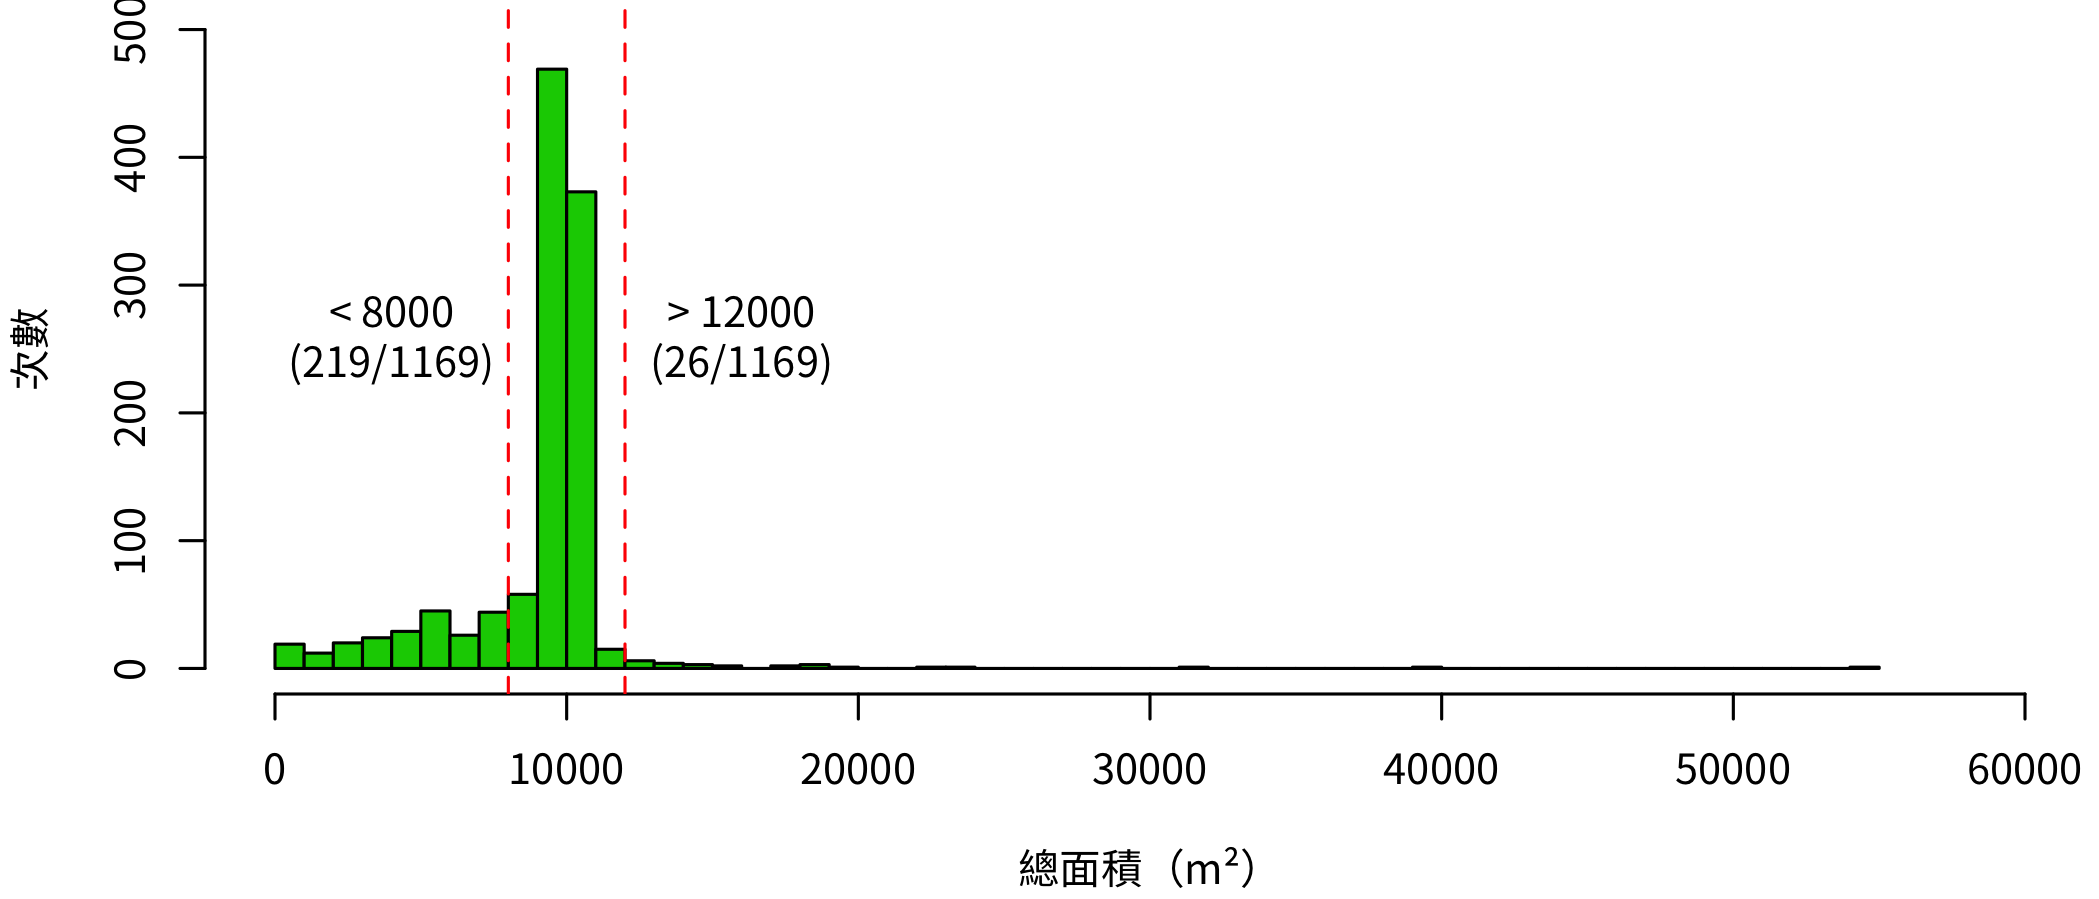
\includegraphics[width=1\textwidth]{invalid-area.png}
\end{center}
\end{frame}

\begin{frame}{過大的未定義面積}
\begin{itemize}
	\item 1169個樣點中有125個樣點之未定義面積大於8,000 m²
	\item 未定義面積過大的樣點對之後的分析可能造成偏誤,需要重新檢查
\end{itemize}
\begin{center}
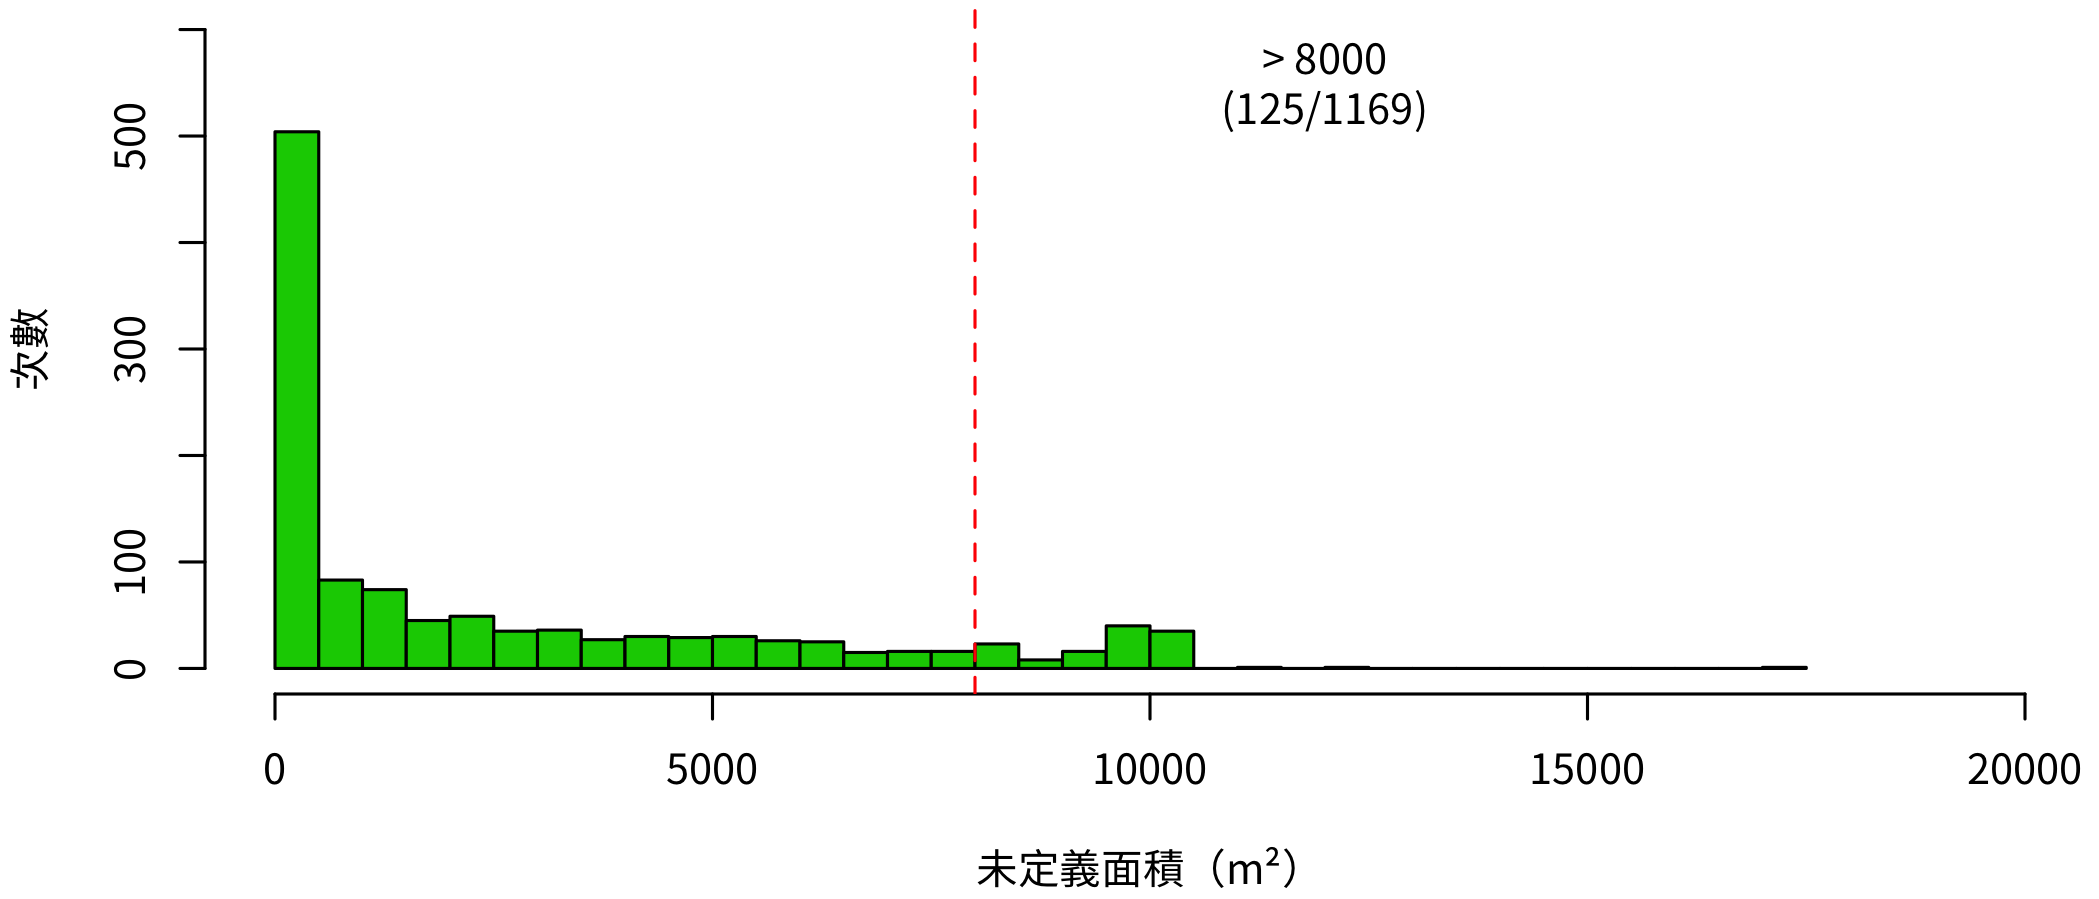
\includegraphics[width=1\textwidth]{invalid-gx-area.png}
\end{center}
\end{frame}

\begin{frame}{面積資料存在太多零}
\begin{columns}[onlytextwidth, c]
	\begin{column}{0.55\textwidth}
	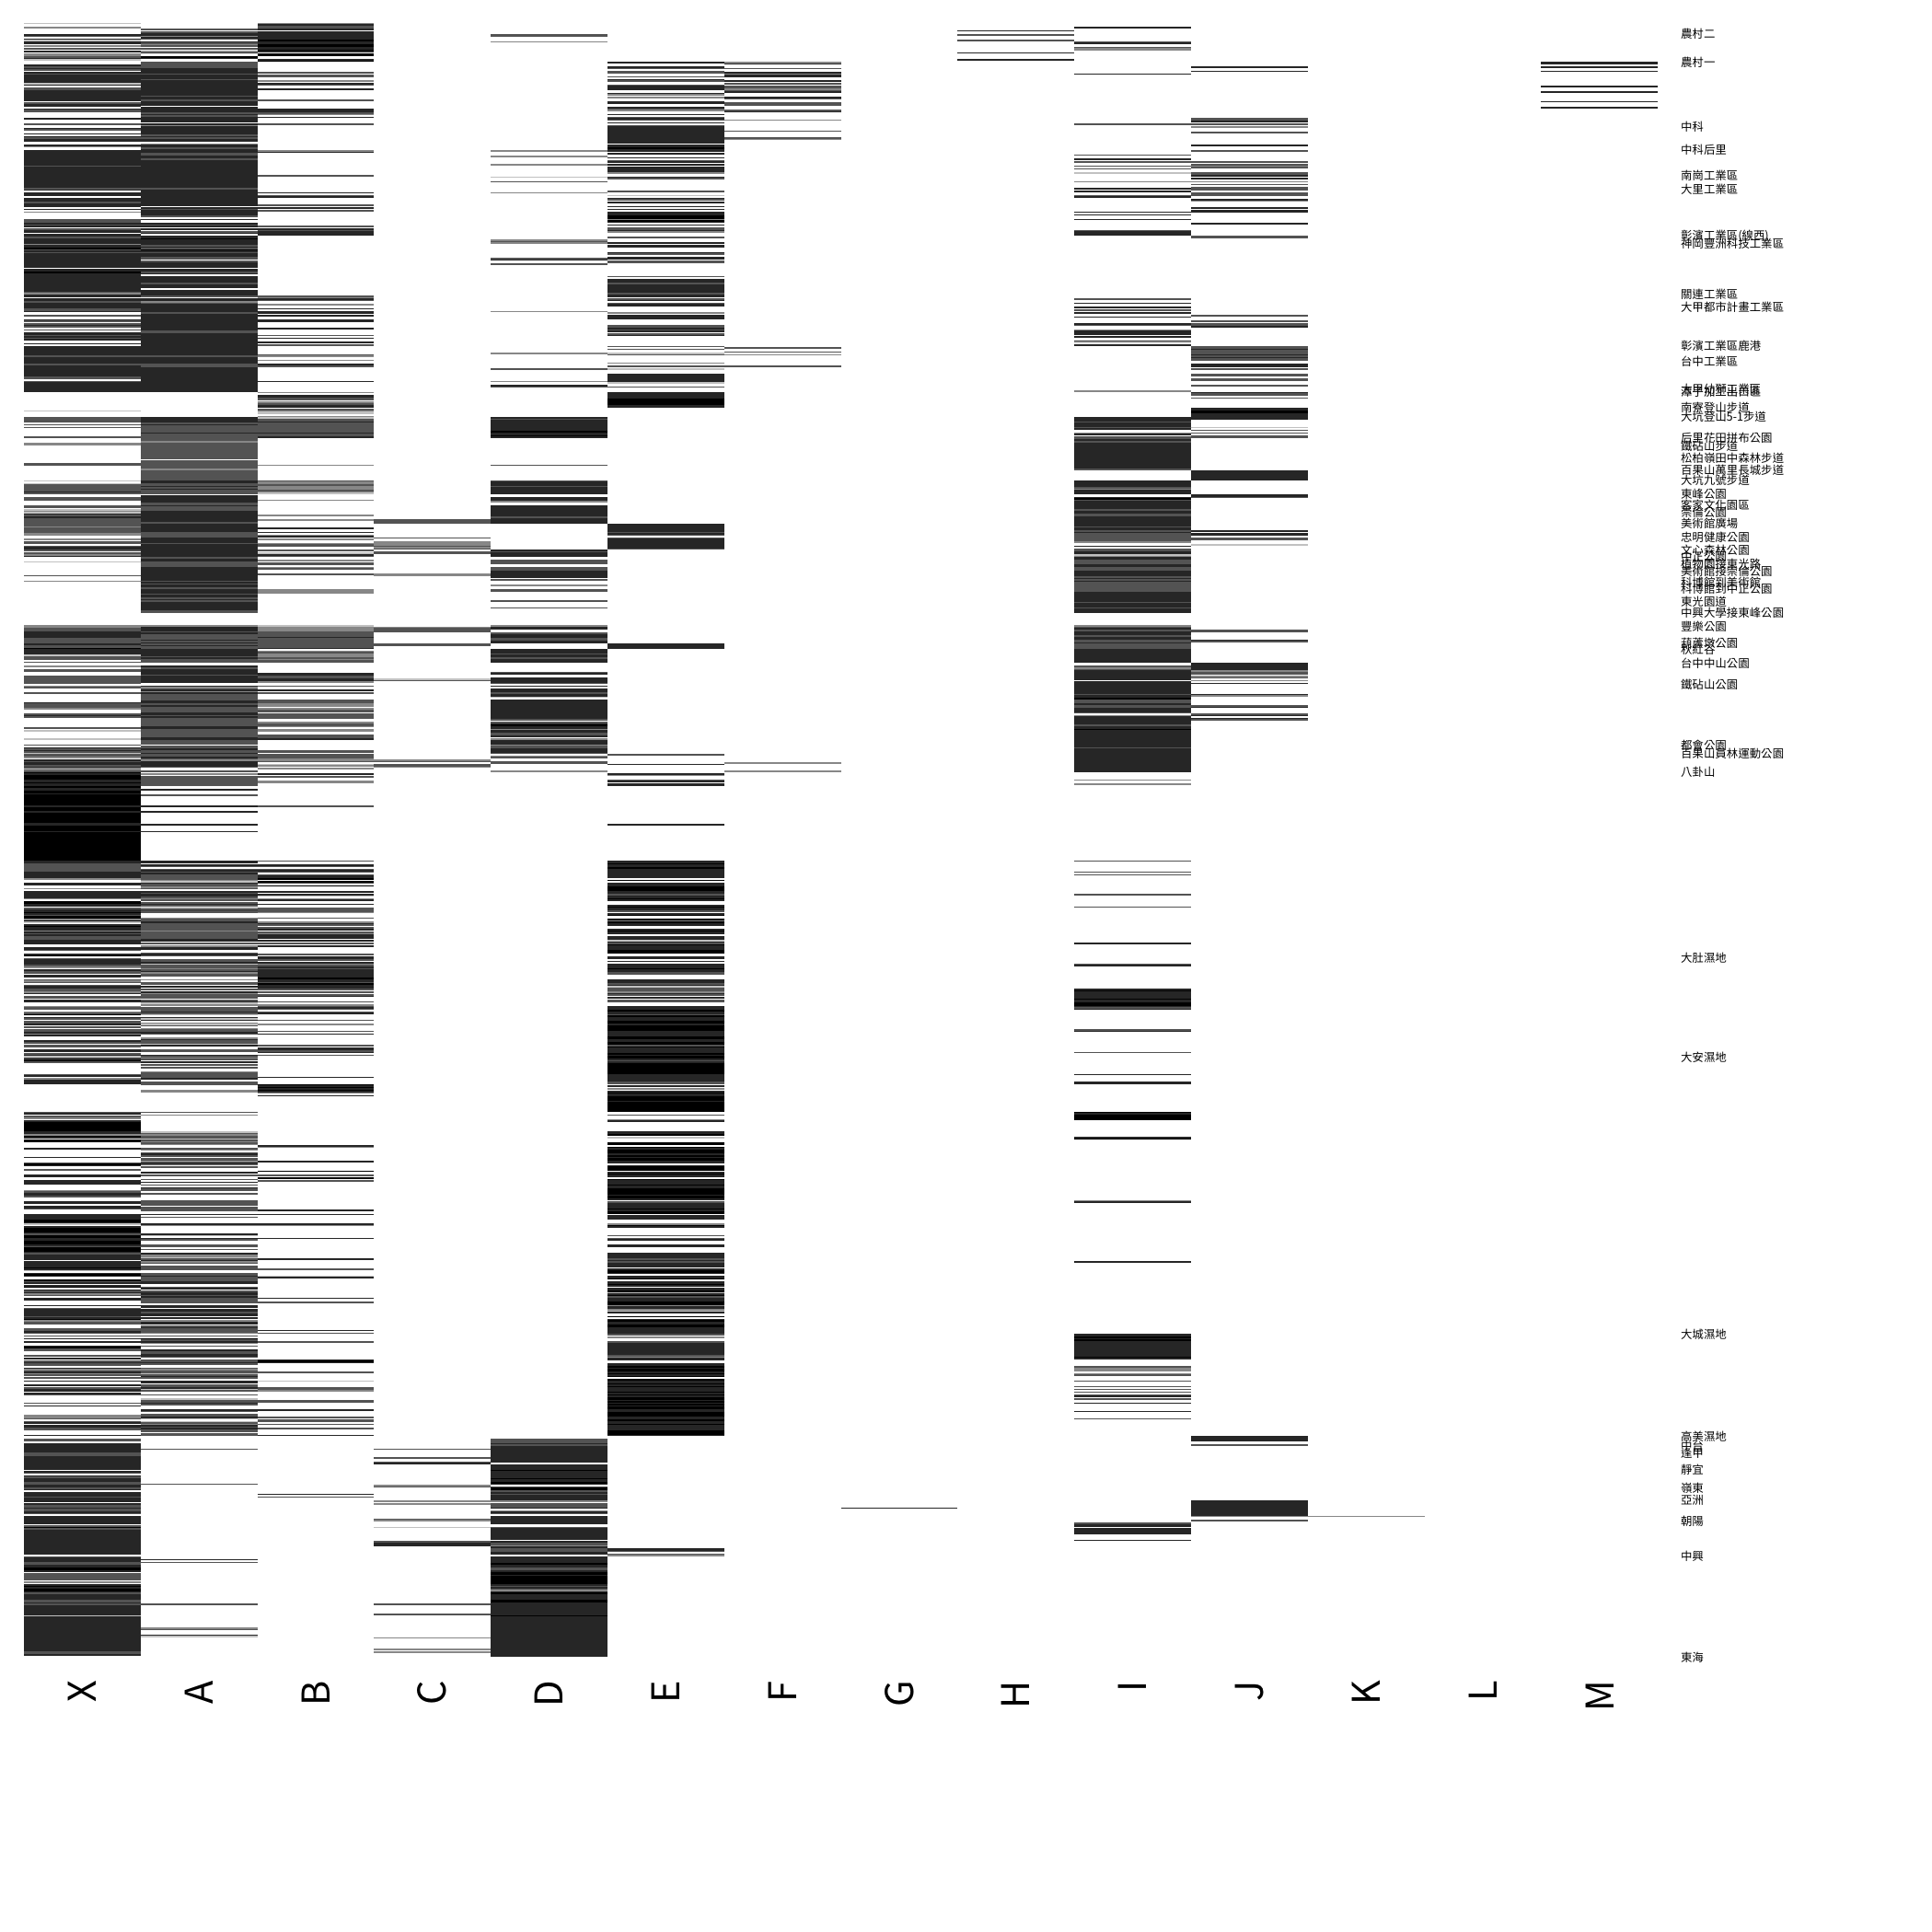
\includegraphics[trim=25 25 25 25, width=1\textwidth]{invalid-type.png}
	\end{column}
	\begin{column}{0.45\textwidth}
		\begin{itemize}
%			\item 左圖顏色越淺表示\alert{同樣點內}面積比例越小,越深表示\alert{同樣點內}面積比例越大,但整列都白色表示全為零
			\item 類型C/F/G/H/K/M零的面積太多
			\item 類型L的面積全為零
			\item 有10個樣點的所有面積資料(包括未定義)全為零,其中有9個樣點屬於豐樂公園,且豐樂公園也只貢獻了10個樣點
			\item 在$1169 \times (13+1)$個面積值中個有9個面積值未填
			\item 上述資料皆需需要重新檢查;若納入分析並沒有貢獻能力或造成偏誤
		\end{itemize}
	\end{column}
\end{columns}
\end{frame}

\begin{frame}{綜觀生態資料}
\begin{columns}[onlytextwidth, c]
	\begin{column}{0.55\textwidth}
	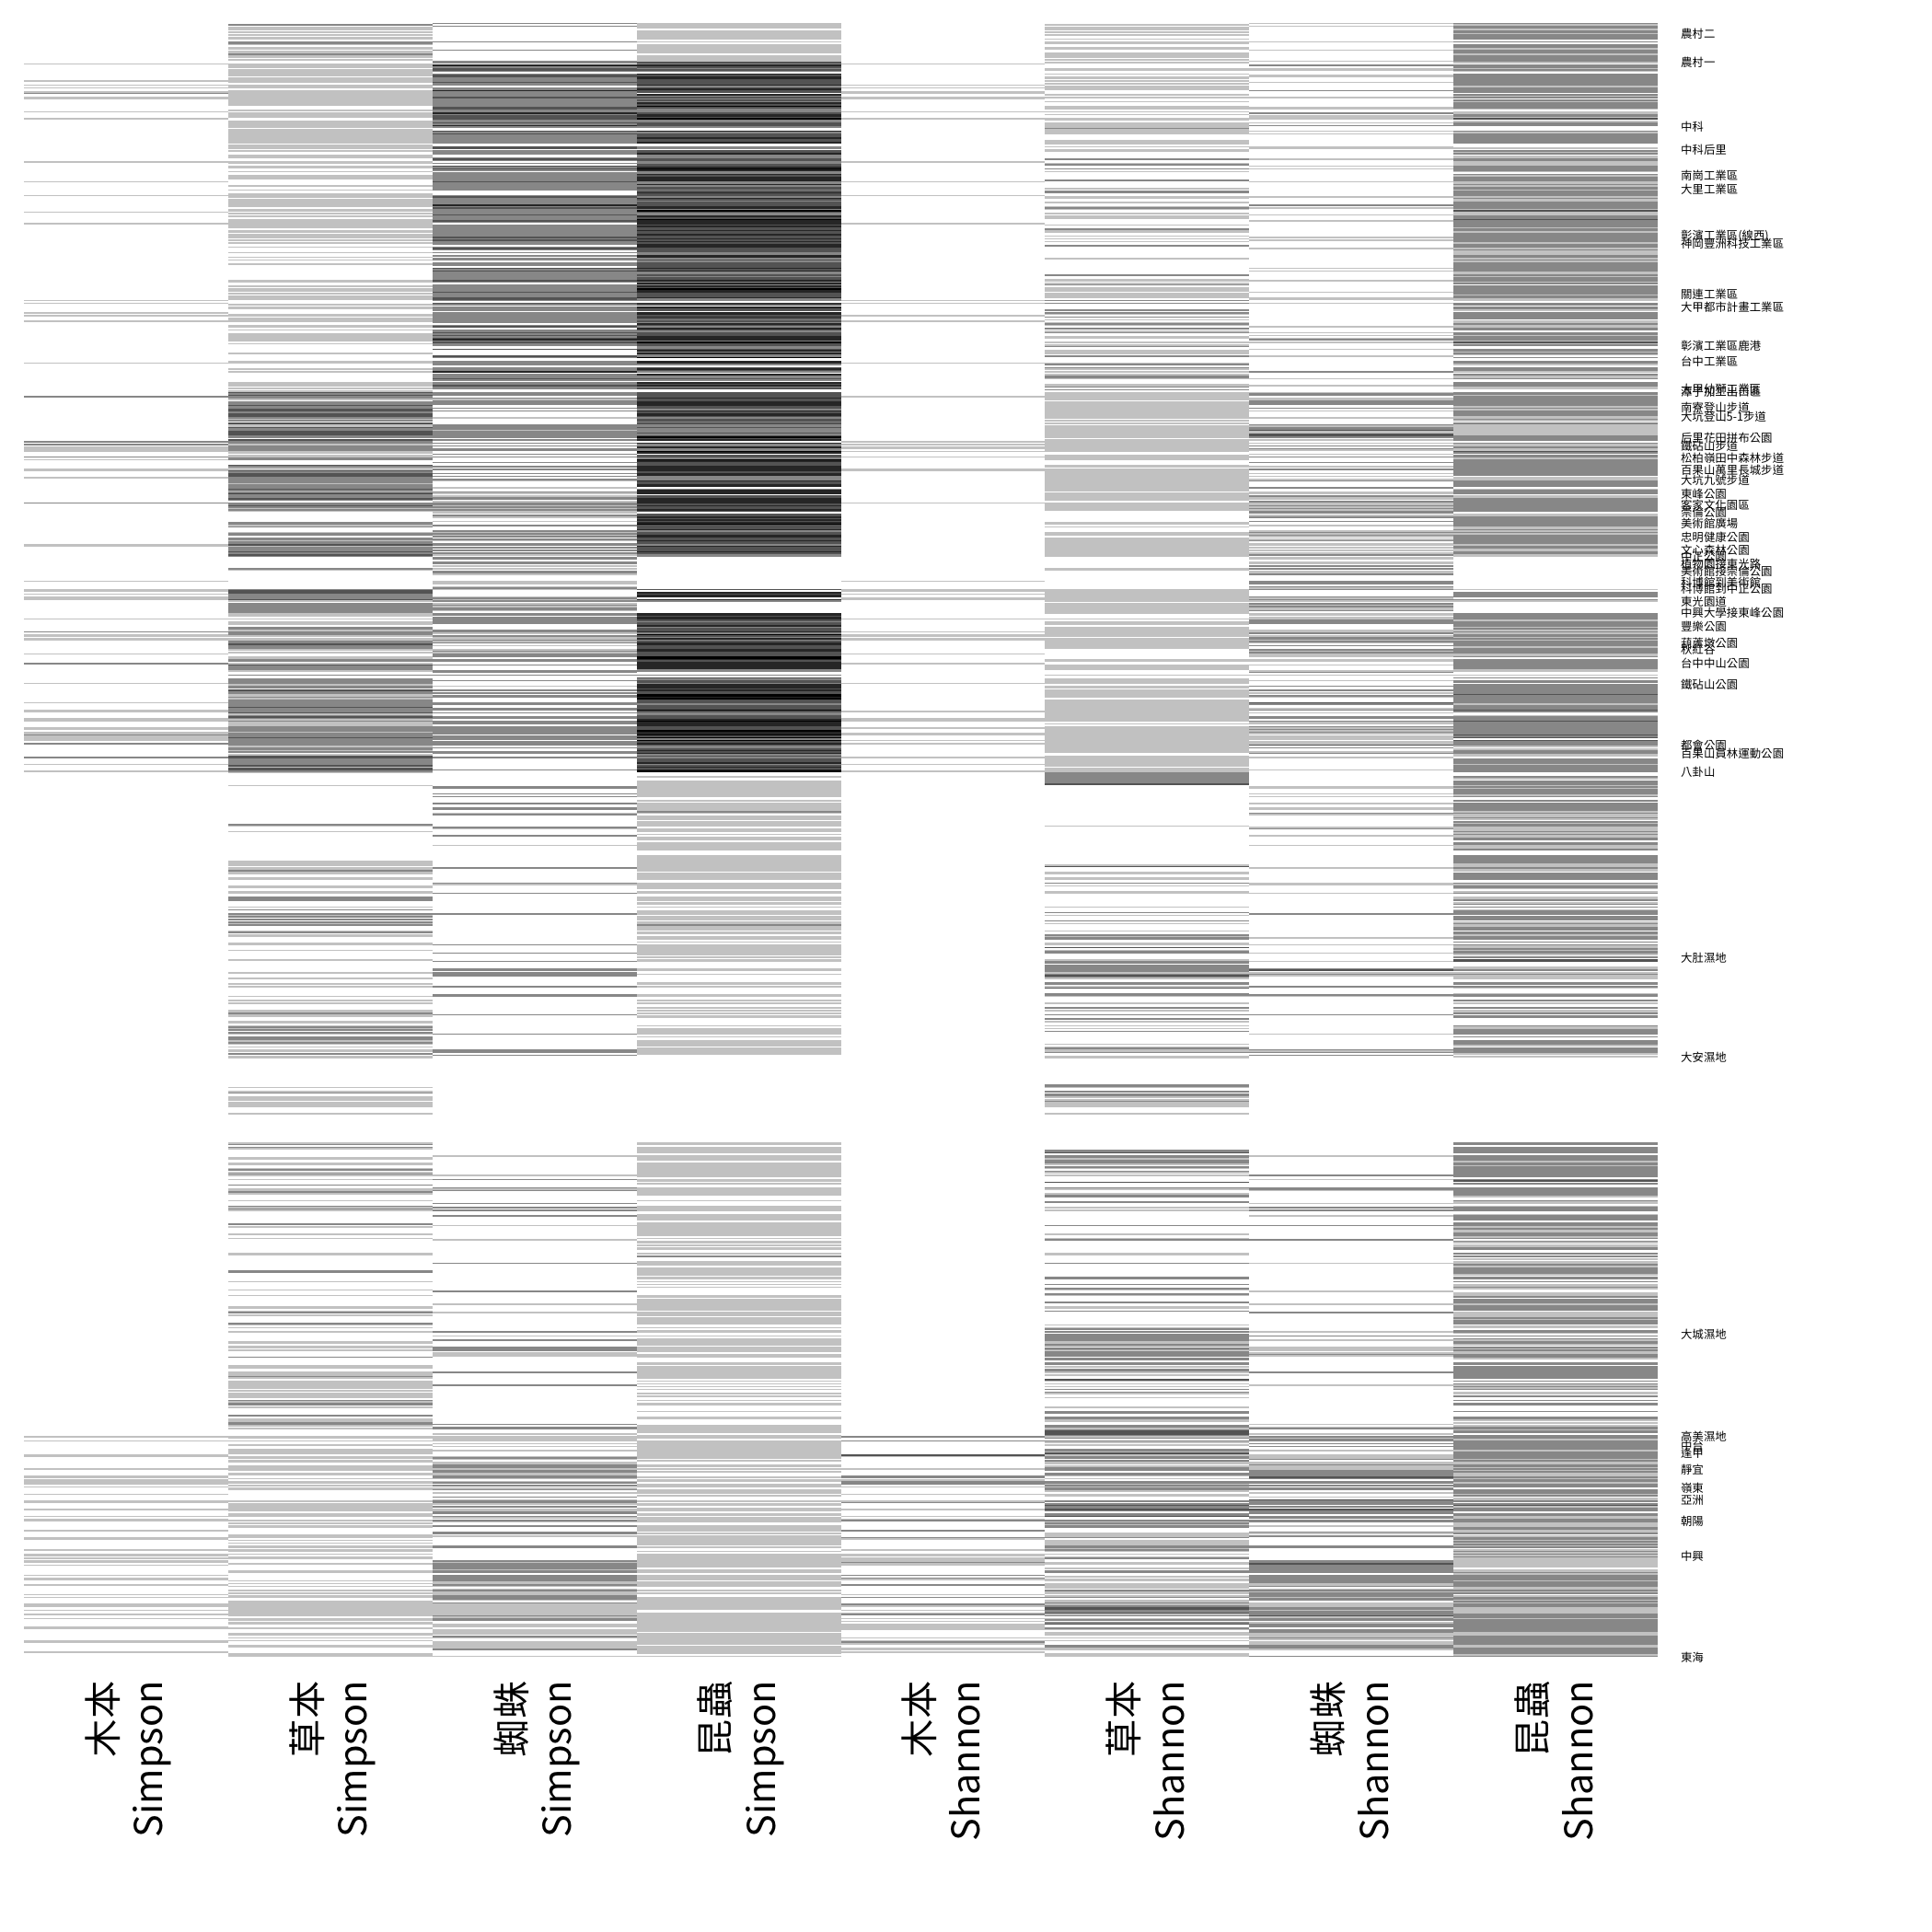
\includegraphics[trim=25 25 25 25, width=1\textwidth]{invalid-bio.png}
	\end{column}
	\begin{column}{0.45\textwidth}
		\begin{itemize}
%			\item 左圖顏色越淺表示\alert{同樣點內}指數數值越小,越深表示\alert{同樣點內}指數數值越大
			\item \sout{三個濕地的多樣性資料有太多零,不存在足夠變異}
			\item \sout{昆蟲或蜘蛛的Simpson與Shannon指數之大小趨勢明顯相反}
			\item Shannon指數的變異比較均勻,而Simpson的變數在昆蟲明顯較大;之後分析若採用昆蟲Simpson指數的原始數字,可能會將昆蟲資料過度放大
			\item 木本資料太多零,排除之
		\end{itemize}
	\end{column}
\end{columns}
\end{frame}

\begin{frame}{Simpson index 大於 1}
\begin{columns}[onlytextwidth, c]
	\begin{column}{0.55\textwidth}
	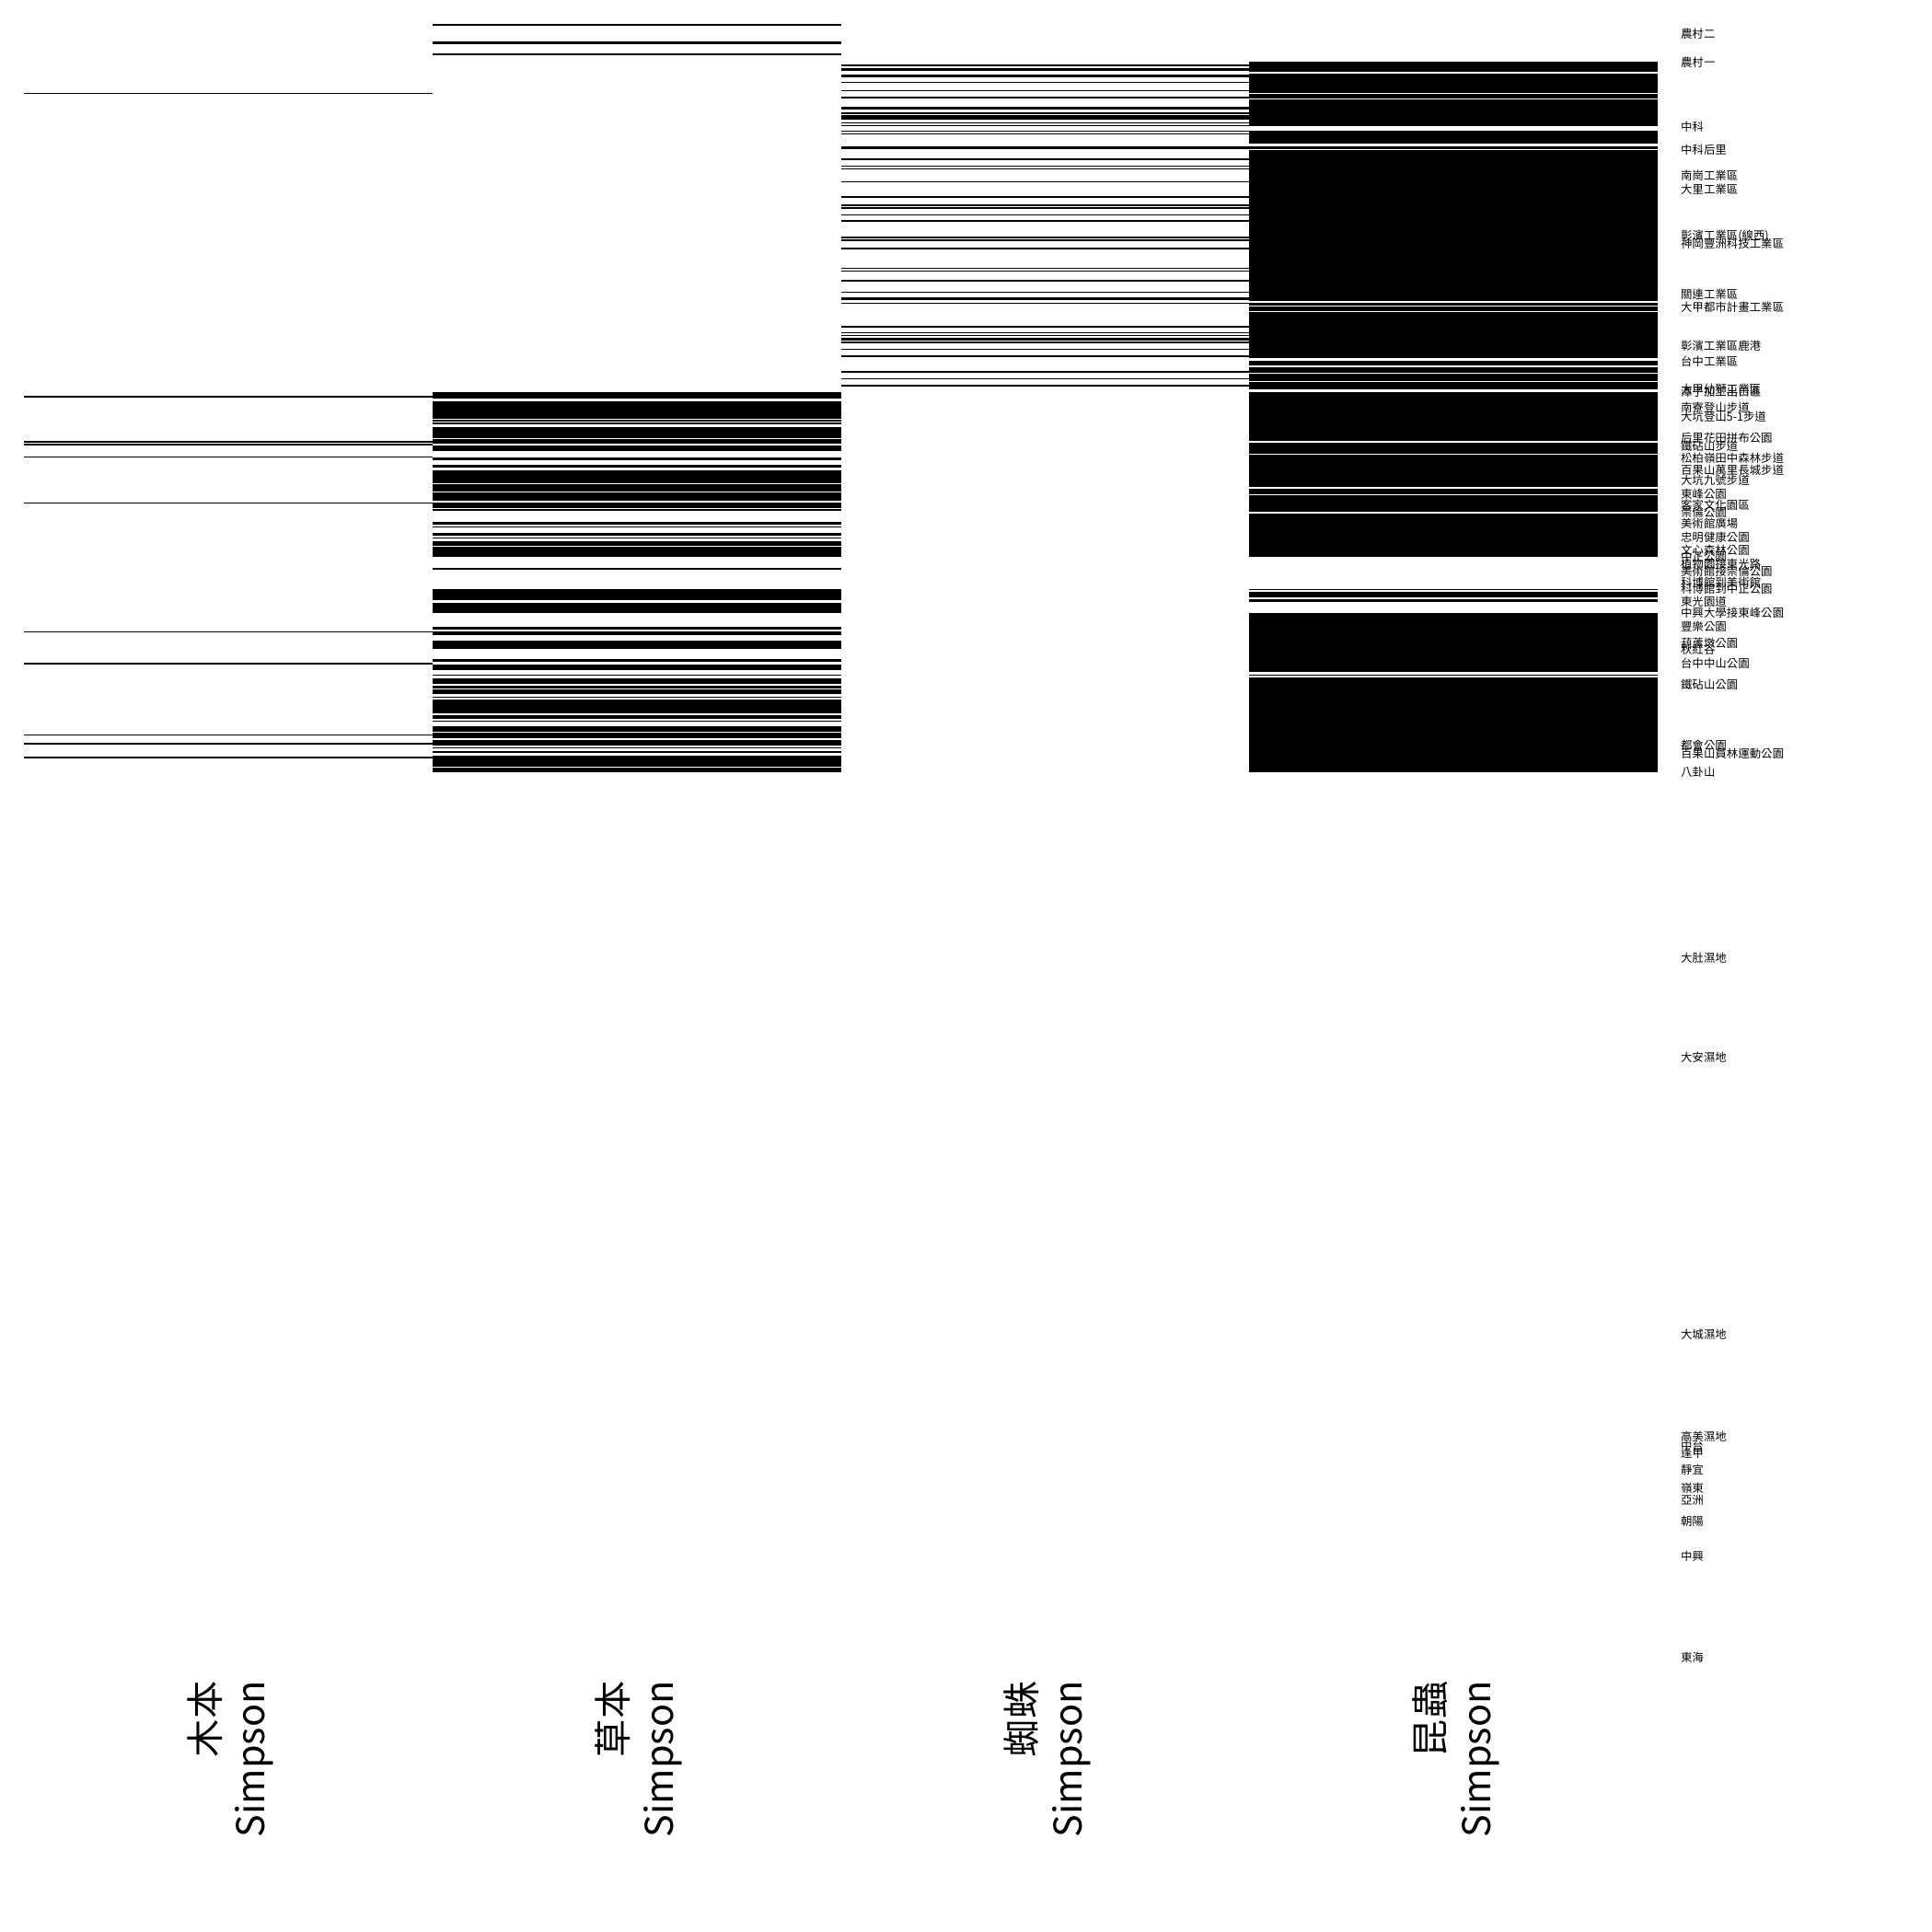
\includegraphics[trim=25 25 25 25, width=1\textwidth]{invalid-bio-simpson.png}
	\end{column}
	\begin{column}{0.45\textwidth}
		\begin{itemize}
			\item 理論上Simpson index不可能大於 1
			\item 4種Simpson index皆有此問題
			\item 博森檢查部份蜘蛛與昆蟲資料後已部份修正
			\item 目前分析尚不採用所有Simpson index
		\end{itemize}
	\end{column}
\end{columns}
\end{frame}


\section{求解侯選之TBAF建構分數}

\begin{frame}{面積資料的挑選與標準化規則}
\begin{enumerate}
	\item 去除存在任何缺失資料的樣點
	\item 去除總面積(包括未定義面積)小於5,000 m²或大於15,000 m²的樣點
	\item 去除未定義面積大於5,000 m²的樣點(剩793個樣點)
	\item 以每樣點為單位,將已定義類型面積和調整為1(即不考慮未定義面積的資訊),再減去平均以中心化
		\[ 
			\frac{g_{jk}}{\mathrm{sum}(g_{j\cdot})} - 
			\mathrm{mean} \left( \frac{g_{jk}}{\mathrm{sum}(g_{j\cdot})} \right)
		\]
	\item 以一次項,二次項及一次項間乘積為解釋變數;太多面積為0的變數直接手動移除
	\item 最後剩下$793\times27$個面積資料,稱為$\mathbf{G}$
\end{enumerate}
\end{frame}


\begin{frame}{生態資料的挑選與標準化規則}
%我按以下規則挑選出之後分析所採用的面積資料:
\begin{enumerate}
	\item 我選用3種Shannon指數(木本資料不考慮),以每種指數為單位,將3項指數最大值為1且最小值為0進行標準化
		\[ \frac{b_{jk}}{\max(b_{\cdot k})} \]
	\item 因為木本Shannon指數的零太多且與其它變數相關低,不再考慮
\end{enumerate}
\end{frame}



\begin{frame}{挑選與調整後的所有變數}
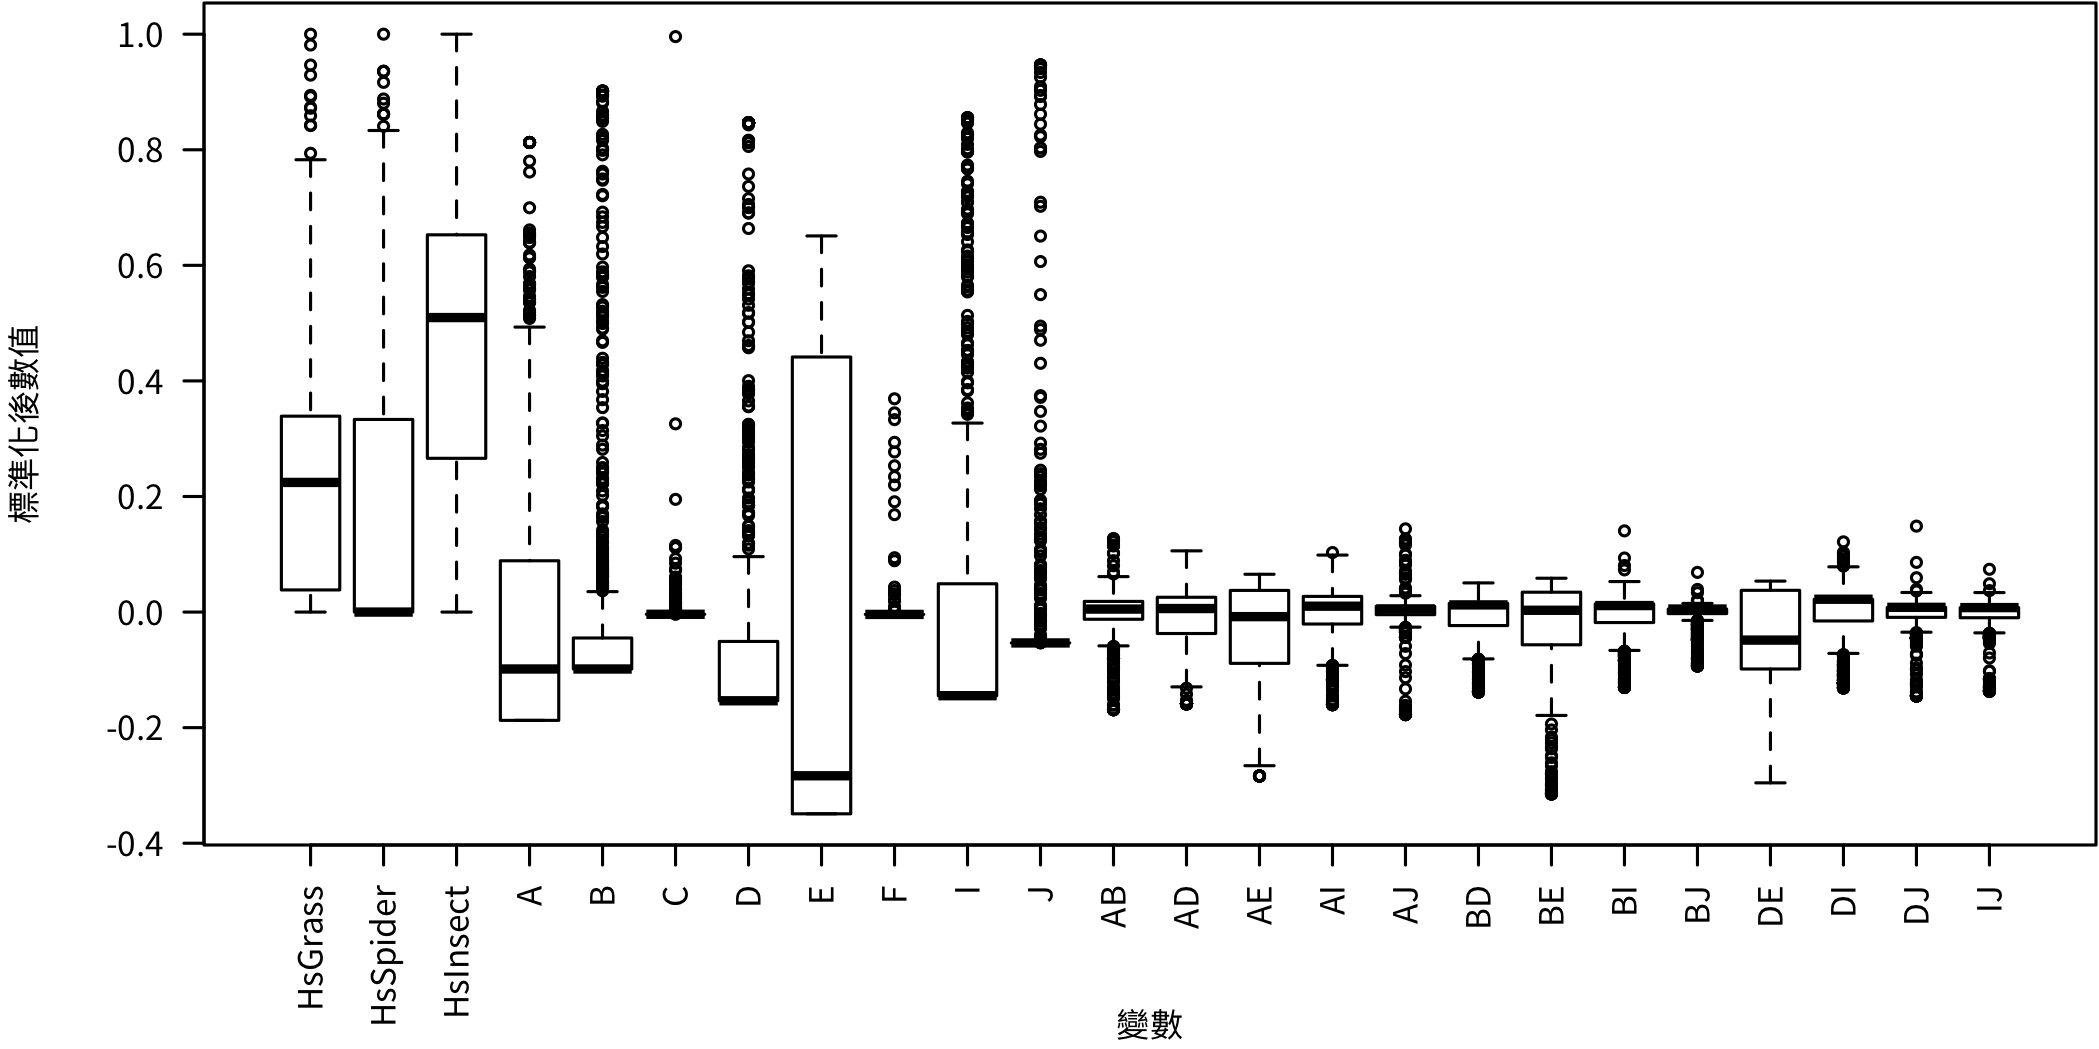
\includegraphics[width=1\textwidth]{var-summary.png}
\end{frame}


\begin{frame}{以複迴歸求解侯選之TBAF建構分數}

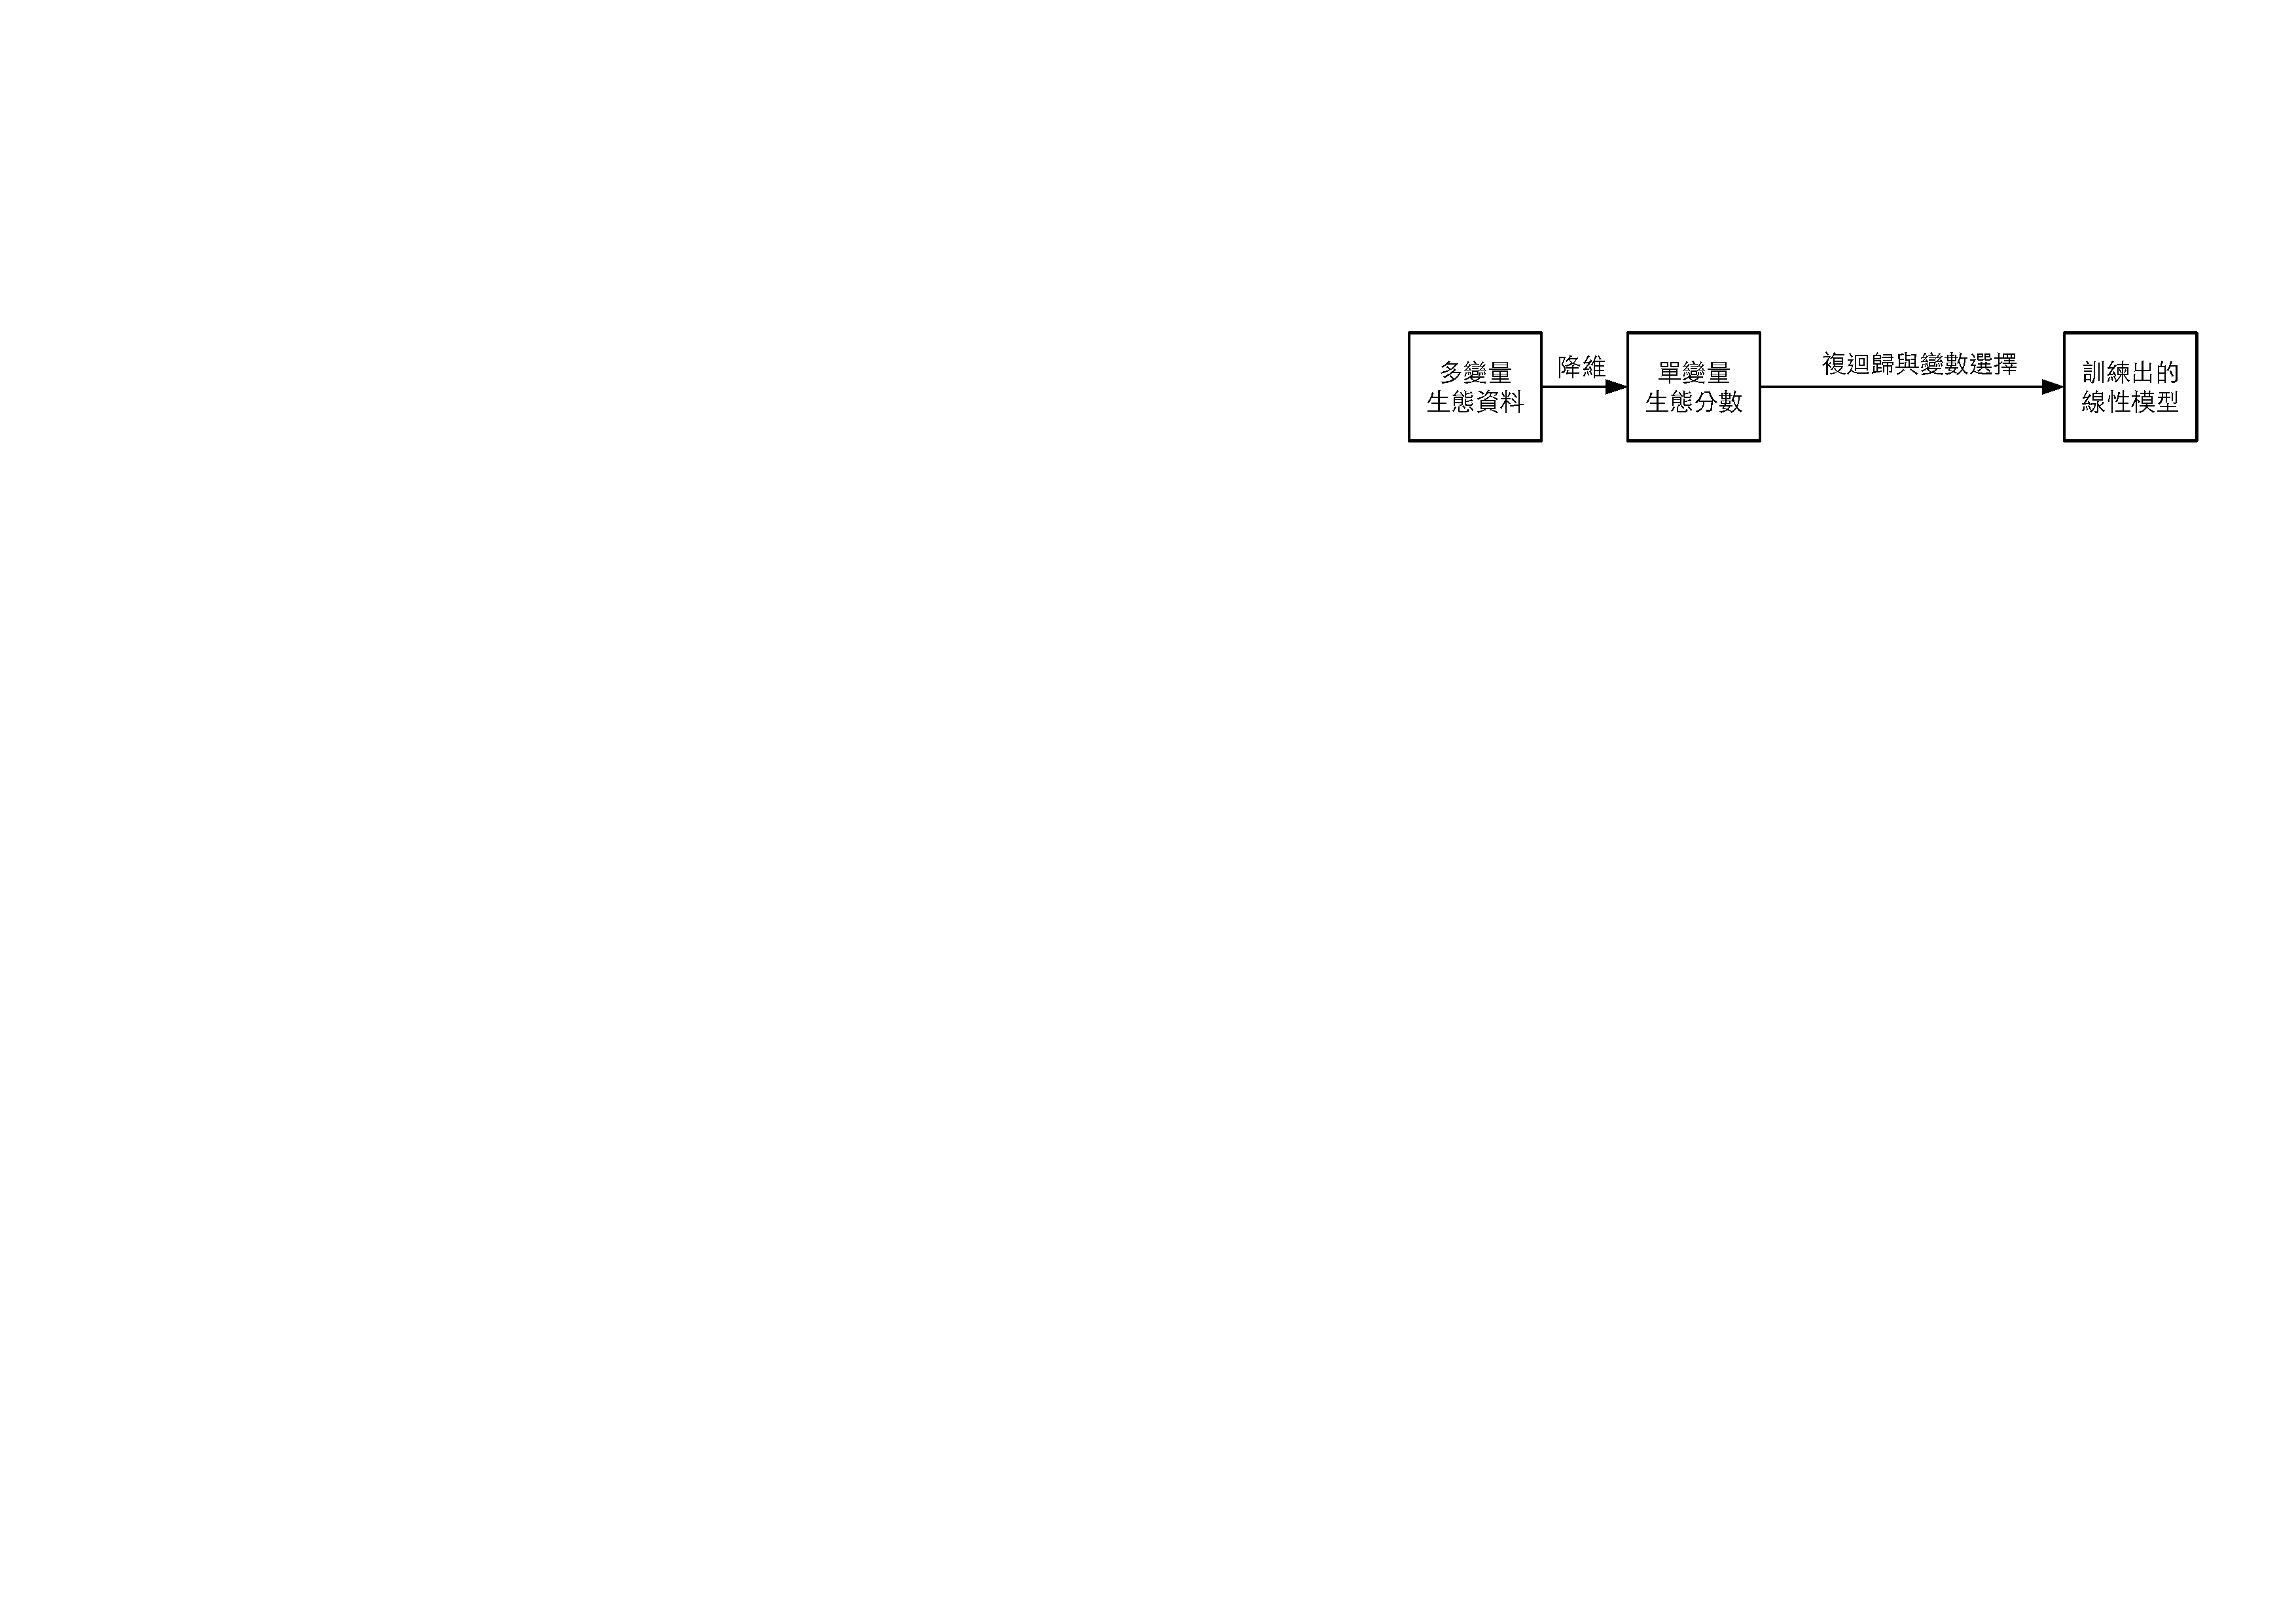
\includegraphics[width=1\textwidth]{diagram-0.pdf}

\begin{enumerate}
\item 利用PCA、FA(1)、MDS(1)、RDA萃取出生態資料的第一空間分數之標準常態分數$\mathbf{S}_i$
\item 以$\mathbf{S}_i$為反應變數,面積分數$\mathbf{G}$為解釋變數,建立4個線性複迴歸模型\[ \mathcal{M}_i : \mathbf{S}_i =  \mathbf{\beta}_i^\top \mathbf{G} + \mathbf{E}_i \]
%\item 以僅含一次項為起點逐次加入或排除一項解釋變數,直到求得最小AIC與最小BIC之最佳模型,產生$4 \times 2 = 8$組侯選TBAF建構分數
\item 採用二種自動化變數挑選方法

	\begin{enumerate}
		\item 以僅包括一次項為起點,每次加入或刪去一項變數,直到找到最小AIC(以下標1表示)
		\item 以包括一次項及交互作用項為起點,每次加入或刪去一項變數,直到找到最小BIC(以下標F表示)
	\end{enumerate}
\item 強迫保留A D E F I五類面積,使各表面型態組皆有資料,不然會「變數沒選到D結果東海都第一名」
\item 得到 $4 \times 2 = 8$ 個迴歸式
\end{enumerate}
\end{frame}

\begin{frame}[fragile]{生態資料降維}
\begin{columns}[onlytextwidth, c]
	\begin{column}{0.5\textwidth}
		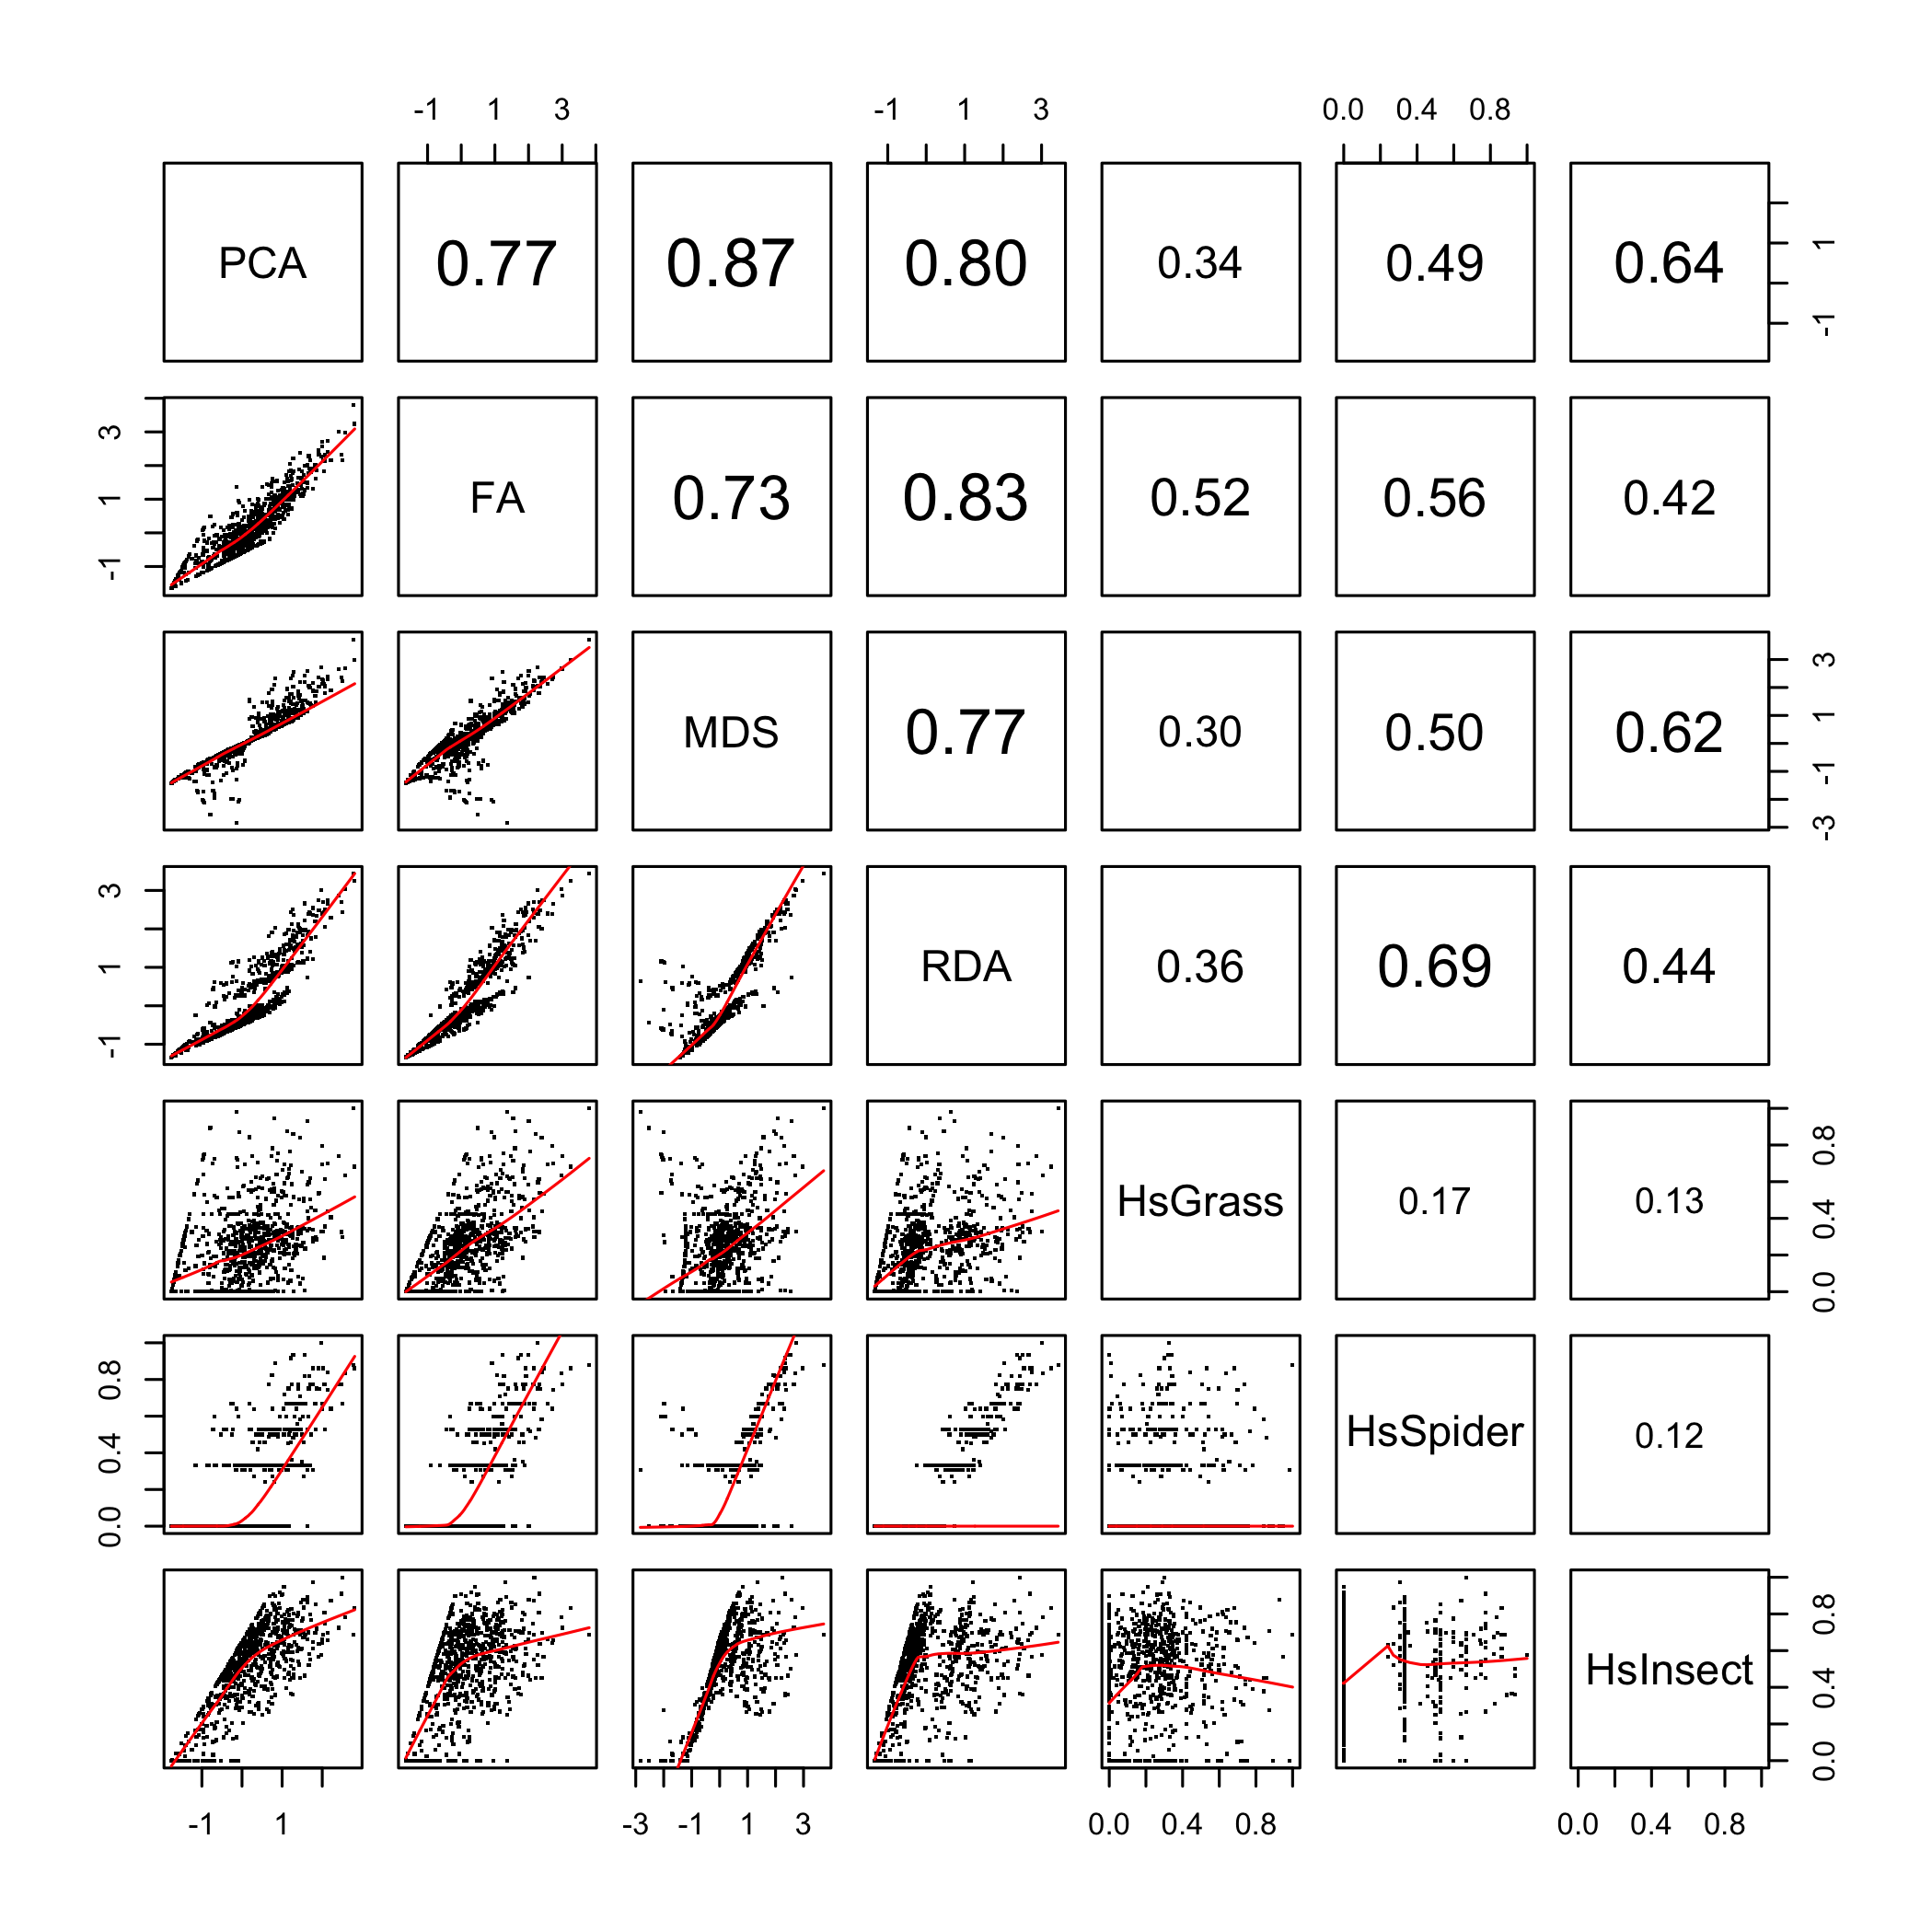
\includegraphics[trim=100 100 100 100, width=1\textwidth]{原始資料降維分數.png}
	\end{column}
	\begin{column}{0.45\textwidth}
		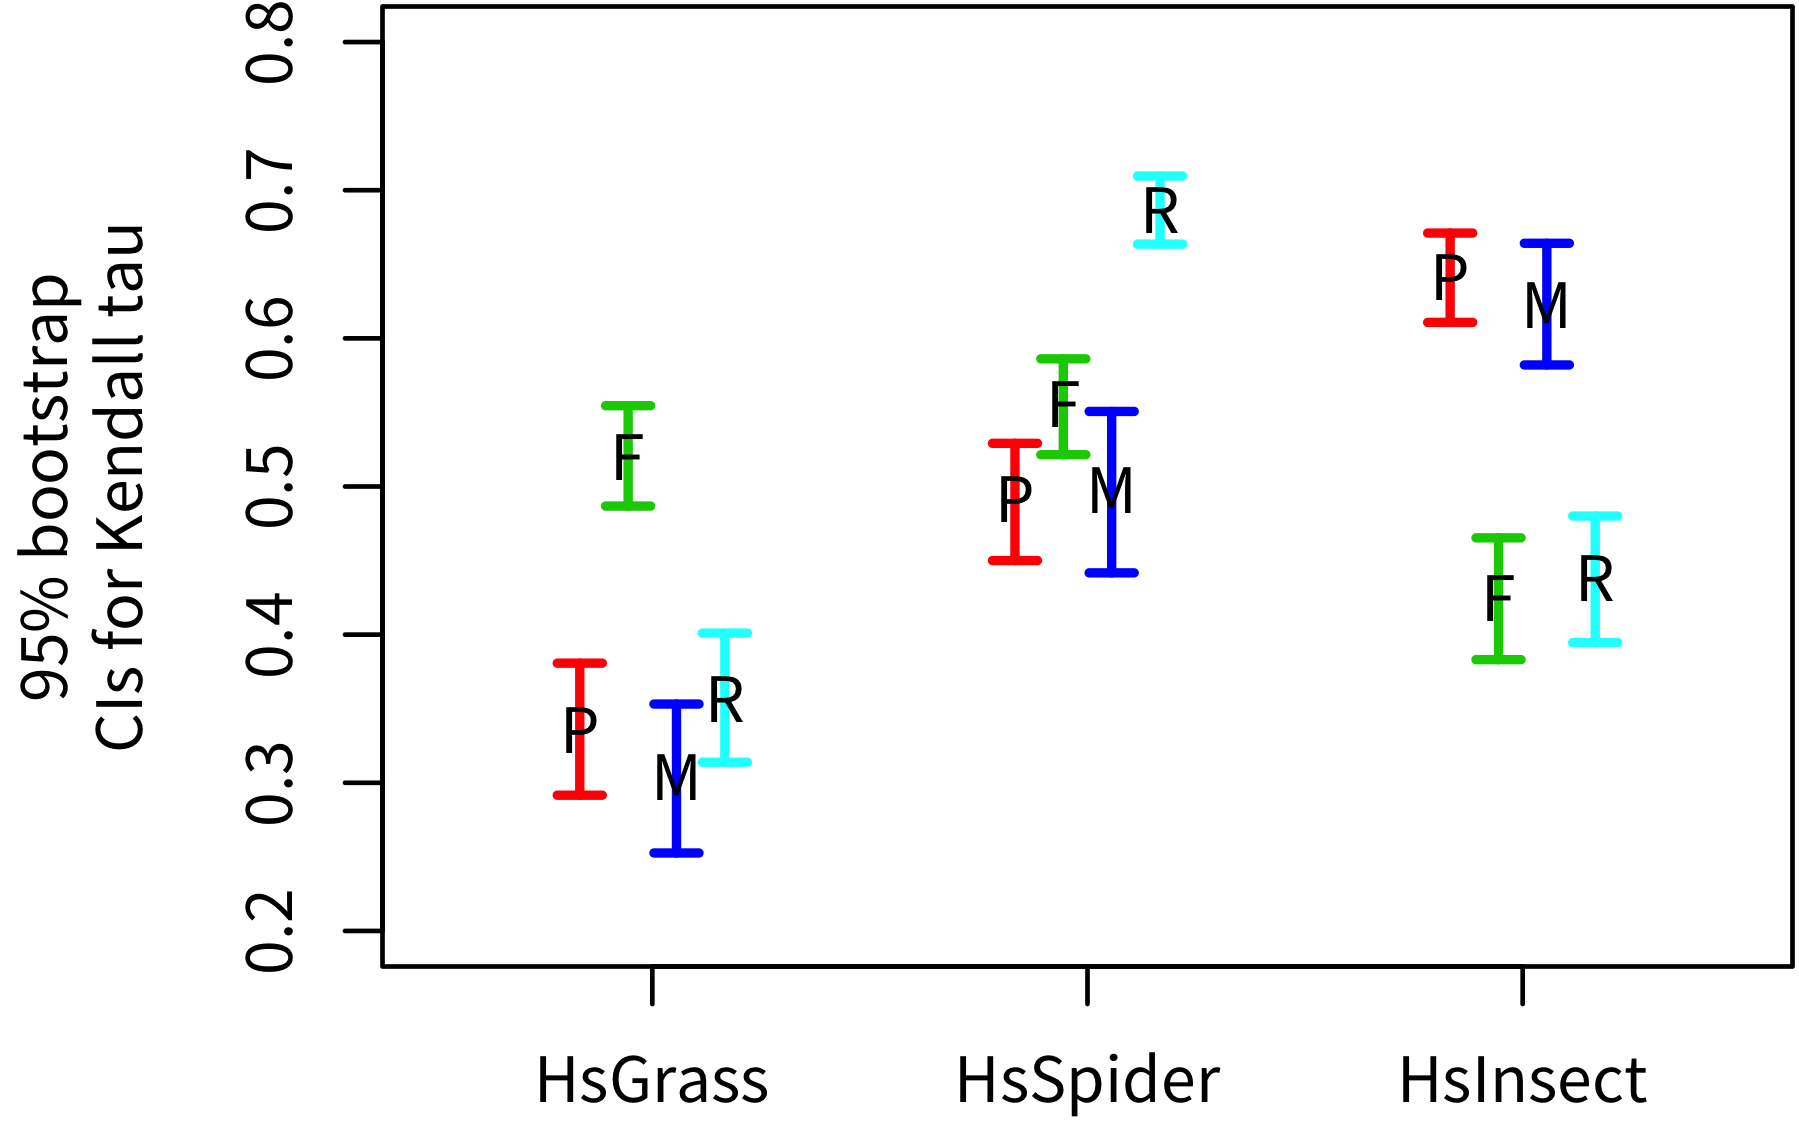
\includegraphics[width=1\textwidth]{bootR-final.png}
		\begin{itemize}
			\item 4種降維方法間呈高度相關
			\item 唯有FA與草本多樣性的相關較高
			\item RDA強調蜘蛛多樣性,其它方法也不太差
			\item PCA和MDS與昆蟲多樣性的相關較高
		\end{itemize}
	\end{column}
\end{columns}
\end{frame}



%\begin{frame}[fragile]{MDS 1\textsuperscript{st} 分數之萃取}
%\begin{Verbatim}[fontsize=\normalsize]
%Stress = 0.284297
%MDS1 loadings
%      HsWood   HsGrass HsSpider HsInsect
%MDS1 0.73107 -0.009557 0.683752 0.207176
%\end{Verbatim}
%\includegraphics[width=1\textwidth]{scoreMDS.png}
%\end{frame}


%\begin{frame}[fragile]{PCA 1\textsuperscript{st} 分數之萃取}
%\begin{Verbatim}[fontsize=\normalsize]
%Variance = 0.5363051
%PC1 loadings
%       HsWood HsGrass HsSpider HsInsect
%[1,] 0.182563 0.36865 0.344669 0.843784
%\end{Verbatim}
%\includegraphics[width=1\textwidth]{scorePCA.png}
%\end{frame}


%\begin{frame}[fragile]{RDA 1\textsuperscript{st} 分數之萃取}
%\begin{Verbatim}[fontsize=\normalsize]
%Variance (residual included) = 0.27726
%Variance (residual excluded) = 0.64011
%RD1 loadings
%       HsWood  HsGrass HsSpider HsInsect
%[1,] 0.411635 0.554657 1.029198  1.51651
%\end{Verbatim}
%\begin{center}
%\includegraphics[width=1\textwidth]{scoreRDA.png}
%\end{center}
%\end{frame}


%\begin{frame}[fragile]{FA 1\textsuperscript{st} 分數之萃取}
%\begin{Verbatim}[fontsize=\normalsize]
%Variance = 0.349
%Factor loadings
%       HsWood  HsGrass HsSpider HsInsect
%F1   0.296305 0.405555 0.383069 0.997497
%\end{Verbatim}
%\includegraphics[width=1\textwidth]{scoreFA.png}
%\end{frame}


%\begin{frame}[fragile]{CCA 1\textsuperscript{st} 分數之萃取}
%\begin{Verbatim}[fontsize=\normalsize]
%Variance = 60.078%
%Canonical correlation = 0.79476
%CC1 loadings
%       HsWood  HsGrass HsSpider HsInsect
%[1,] 0.677566 0.007338 4.063898 0.354358
%\end{Verbatim}
%\includegraphics[width=1\textwidth]{scoreCCA.png}
%% 因為1\textsuperscript{st} CCA分數表現不太好,且之後複迴歸分析時產生完美之後不再考慮。
%\end{frame}




\begin{frame}[label=coef]{複迴歸及變數選擇後的原始迴歸係數(侯選之TBAF建構分數)}
% latex table generated in R 3.2.2 by xtable 1.8-0 package
% Wed Nov 18 06:06:08 2015
\begin{table}[ht]
\centering
{\small
\begin{mytabular}{lrrrrrrrr}
  \hline
 & PCA\textsubscript{1} & PCA\textsubscript{F} & FA\textsubscript{1} & FA\textsubscript{F} & MDS\textsubscript{1} & MDS\textsubscript{F} & RDA\textsubscript{1} & RDA\textsubscript{F} \\ 
  \hline
Int. & 0.045 & 0.045 & 0.050 & 0.050 & $-$0.010 & $-$0.040 & 0.045 & 0.079 \\ 
  $ A $ & 0.336 & 0.336 & 0.218 & 0.218 & $-$0.171 & $-$0.202 & 0.350 & 1.333 \\ 
   $A \times B $ &  &  &  &  &  &  &  & 1.404 \\ 
   $A \times D $ & $-$2.167 & $-$2.167 &  &  & $-$2.835 & $-$2.833 &  &  \\ 
   $A \times E $ & 1.753 & 1.753 & 1.503 & 1.503 & 1.107 & 1.082 & 1.216 & 1.326 \\ 
   $A \times I $ & 2.671 & 2.671 & 2.457 & 2.457 &  &  & 3.014 & 3.117 \\ 
   $A \times J $ &  &  & $-$2.161 & $-$2.161 & $-$1.799 & $-$1.897 & $-$2.117 & $-$1.933 \\ 
  $ B $ &  &  &  &  &  &  &  & 1.329 \\ 
   $B \times E $ &  &  &  &  &  &  &  & 1.142 \\ 
  $ C $ &  &  &  &  &  &  &  & 1.640 \\ 
  $ D $ & 0.900 & 0.900 & 1.036 & 1.036 & 0.893 & 0.860 & 1.325 & 2.190 \\ 
   $D \times I $ & 2.551 & 2.551 &  &  & 1.365 & 1.369 &  &  \\ 
  $ E $ & $-$0.016 & $-$0.016 & $-$0.090 & $-$0.090 & $-$0.044 & $-$0.085 & $-$0.084 & 0.890 \\ 
  $ F $ & $-$0.324 & $-$0.324 & $-$0.187 & $-$0.187 & $-$0.413 & $-$0.499 & 0.077 & 1.328 \\ 
  $ I $ & 0.666 & 0.666 & 0.311 & 0.311 & 0.282 & 0.007 & 0.493 & 1.378 \\ 
   $I \times J $ &  &  &  &  &  & $-$4.881 &  &  \\ 
  $ J $ & 0.963 & 0.963 & 0.745 & 0.745 & 0.752 &  & 0.743 & 1.647 \\ 
   \hline
\end{mytabular}
}
\end{table}

\end{frame}


\begin{frame}[label=coef]{解釋變數之VIF}
%VIF越小越好;超過5要小心。
% latex table generated in R 3.2.2 by xtable 1.8-0 package
% Wed Nov 18 06:06:08 2015
\begin{table}[ht]
\centering
{\small
\begin{mytabular}{lrrrrrrrr}
  \hline
 & PCA\textsubscript{1} & PCA\textsubscript{F} & FA\textsubscript{1} & FA\textsubscript{F} & MDS\textsubscript{1} & MDS\textsubscript{F} & RDA\textsubscript{1} & RDA\textsubscript{F} \\ 
  \hline
$ A $ & 4.4 & 4.4 & 3.4 & 3.4 & 4.2 & 4.1 & 3.4 & 28.3 \\ 
   $A \times B $ &  &  &  &  &  &  &  & 1.7 \\ 
   $A \times D $ & 4.1 & 4.1 &  &  & 4.1 & 4.2 &  &  \\ 
   $A \times E $ & 2.2 & 2.2 & 2.2 & 2.2 & 2.2 & 2.2 & 2.2 & 2.3 \\ 
   $A \times I $ & 1.8 & 1.8 & 1.8 & 1.8 &  &  & 1.8 & 1.8 \\ 
   $A \times J $ &  &  & 1.8 & 1.8 & 1.8 & 1.8 & 1.8 & 1.9 \\ 
  $ B $ &  &  &  &  &  &  &  & 27.0 \\ 
   $B \times E $ &  &  &  &  &  &  &  & 3.5 \\ 
  $ C $ &  &  &  &  &  &  &  & 1.7 \\ 
  $ D $ & 4.8 & 4.8 & 2.4 & 2.4 & 4.7 & 4.6 & 2.4 & 44.7 \\ 
   $D \times I $ & 2.4 & 2.4 &  &  & 2.4 & 2.4 &  &  \\ 
  $ E $ & 4.1 & 4.1 & 4.1 & 4.1 & 4.2 & 3.9 & 4.1 & 78.0 \\ 
  $ F $ & 1.1 & 1.1 & 1.1 & 1.1 & 1.1 & 1.1 & 1.1 & 2.0 \\ 
  $ I $ & 3.2 & 3.2 & 2.5 & 2.5 & 2.7 & 2.5 & 2.5 & 34.2 \\ 
   $I \times J $ &  &  &  &  &  & 2.4 &  &  \\ 
  $ J $ & 1.5 & 1.5 & 2.3 & 2.3 & 2.3 &  & 2.3 & 18.2 \\ 
   \hline
\end{mytabular}
}
\end{table}

\centering RDA\textsubscript{F}有嚴重共線性,應不考慮
\end{frame}




%\begin{frame}{PCA分數複迴歸挑選變數後迴歸係數}
%\includegraphics[width=1\textwidth]{beta-PCA.png}
%\end{frame}
%
%\begin{frame}{FA分數複迴歸挑選變數後迴歸係數}
%\includegraphics[width=1\textwidth]{beta-FA.png}
%\end{frame}
%
%\begin{frame}{MDS分數複迴歸挑選變數後迴歸係數}
%\includegraphics[width=1\textwidth]{beta-MDS.png}
%\end{frame}
%
%\begin{frame}{RDA分數複迴歸挑選變數後迴歸係數}
%\includegraphics[width=1\textwidth]{beta-RDA.png}
%\end{frame}



%\begin{frame}[fragile, allowframebreaks]{複迴歸及變數選擇後的標準化迴歸係數}
%若不考慮過去已知的專家分數,下述8組係數可視為侯選之TBAF建構分數
%\begin{table}[ht]
%\centering
%\scriptsize
%\addfontfeatures{Numbers={Monospaced}}
%\rowcolors[]{3}{blue!10}{blue!0} % \rowcolors is  in the xcolor manual
%\begin{tabular}{lrrrrrrrr}
%  \hline
% & PCA.AIC & FA.AIC & MDS.AIC & RDA.AIC & PCA.BIC & FA.BIC & MDS.BIC & RDA.BIC \\
%  \hline
%(Intercept) &  &  &  &  &  &  &  &  \\ 
%  Ga & 0.15 & 0.17 & 0.07 & 0.15 & 0.16 &  &  & 0.14 \\ 
%  Ga2 & -0.14 & -0.20 & -0.12 &  & -0.13 &  &  &  \\ 
%  GaGb &  &  & 0.07 & 0.16 &  &  &  & 0.13 \\ 
%  GaGd & -0.34 & -0.39 & -0.35 & -0.24 & -0.30 & -0.33 & -0.31 & -0.25 \\ 
%  GaGe &  & -0.09 &  & 0.20 &  &  &  & 0.20 \\ 
%  GaGi & 0.05 &  & 0.06 & 0.10 &  &  &  & 0.09 \\ 
%  GaGj & -0.06 & -0.06 & -0.10 &  &  &  & -0.08 &  \\ 
%  Gb &  & -0.15 &  & -0.13 &  &  &  &  \\ 
%  Gb2 & 0.12 & 0.24 & 0.33 & 0.49 &  &  &  & 0.27 \\ 
%  GbGe &  &  & 0.17 & 0.27 &  &  &  & 0.23 \\ 
%  GbGi & 0.09 &  & 0.11 & 0.14 &  &  &  & 0.13 \\ 
%  GbGj & 0.11 & 0.10 & 0.14 & 0.11 &  &  &  &  \\ 
%  Gc & 0.07 & 0.06 & 0.06 &  & 0.07 &  & 0.07 &  \\ 
%  Gd & 0.92 & 0.89 & 0.87 & 0.89 & 0.73 & 0.96 & 0.77 & 0.91 \\ 
%  Gd2 & -0.43 & -0.39 & -0.50 & -0.37 & -0.55 & -0.39 & -0.55 & -0.38 \\ 
%  GdGe & 0.32 & 0.39 & 0.24 & 0.46 &  & 0.53 &  & 0.45 \\ 
%  GdGi & 0.07 & 0.07 &  &  &  &  &  &  \\ 
%  Ge2 & 0.07 &  & 0.11 & 0.27 &  &  &  & 0.29 \\ 
%  GeGi & -0.14 & -0.26 & -0.12 &  &  & -0.35 & -0.08 &  \\ 
%  GeGj & 0.46 & 0.42 & 0.47 & 0.45 & 0.56 & 0.43 & 0.56 & 0.46 \\ 
%  Gi2 &  & -0.18 &  &  &  & -0.35 &  &  \\ 
%  Gj & 0.74 & 0.67 & 0.75 & 0.64 & 0.79 & 0.60 & 0.77 & 0.57 \\ 
%   \hline
%\end{tabular}
%\end{table}
%\end{frame}


%\begin{frame}{PCA分數複迴歸挑選變數後標準化迴歸係數}
%\includegraphics[width=1\textwidth]{beta-stdPCA.png}
%\end{frame}
%
%\begin{frame}{FA分數複迴歸挑選變數後標準化迴歸係數}
%\includegraphics[width=1\textwidth]{beta-stdFA.png}
%\end{frame}
%
%\begin{frame}{MDS分數複迴歸挑選變數後標準化迴歸係數}
%\includegraphics[width=1\textwidth]{beta-stdMDS.png}
%\end{frame}
%
%\begin{frame}{RDA分數複迴歸挑選變數後標準化迴歸係數}
%\includegraphics[width=1\textwidth]{beta-stdRDA.png}
%\end{frame}


\begin{frame}{解釋變數的相對$R^2$貢獻量}
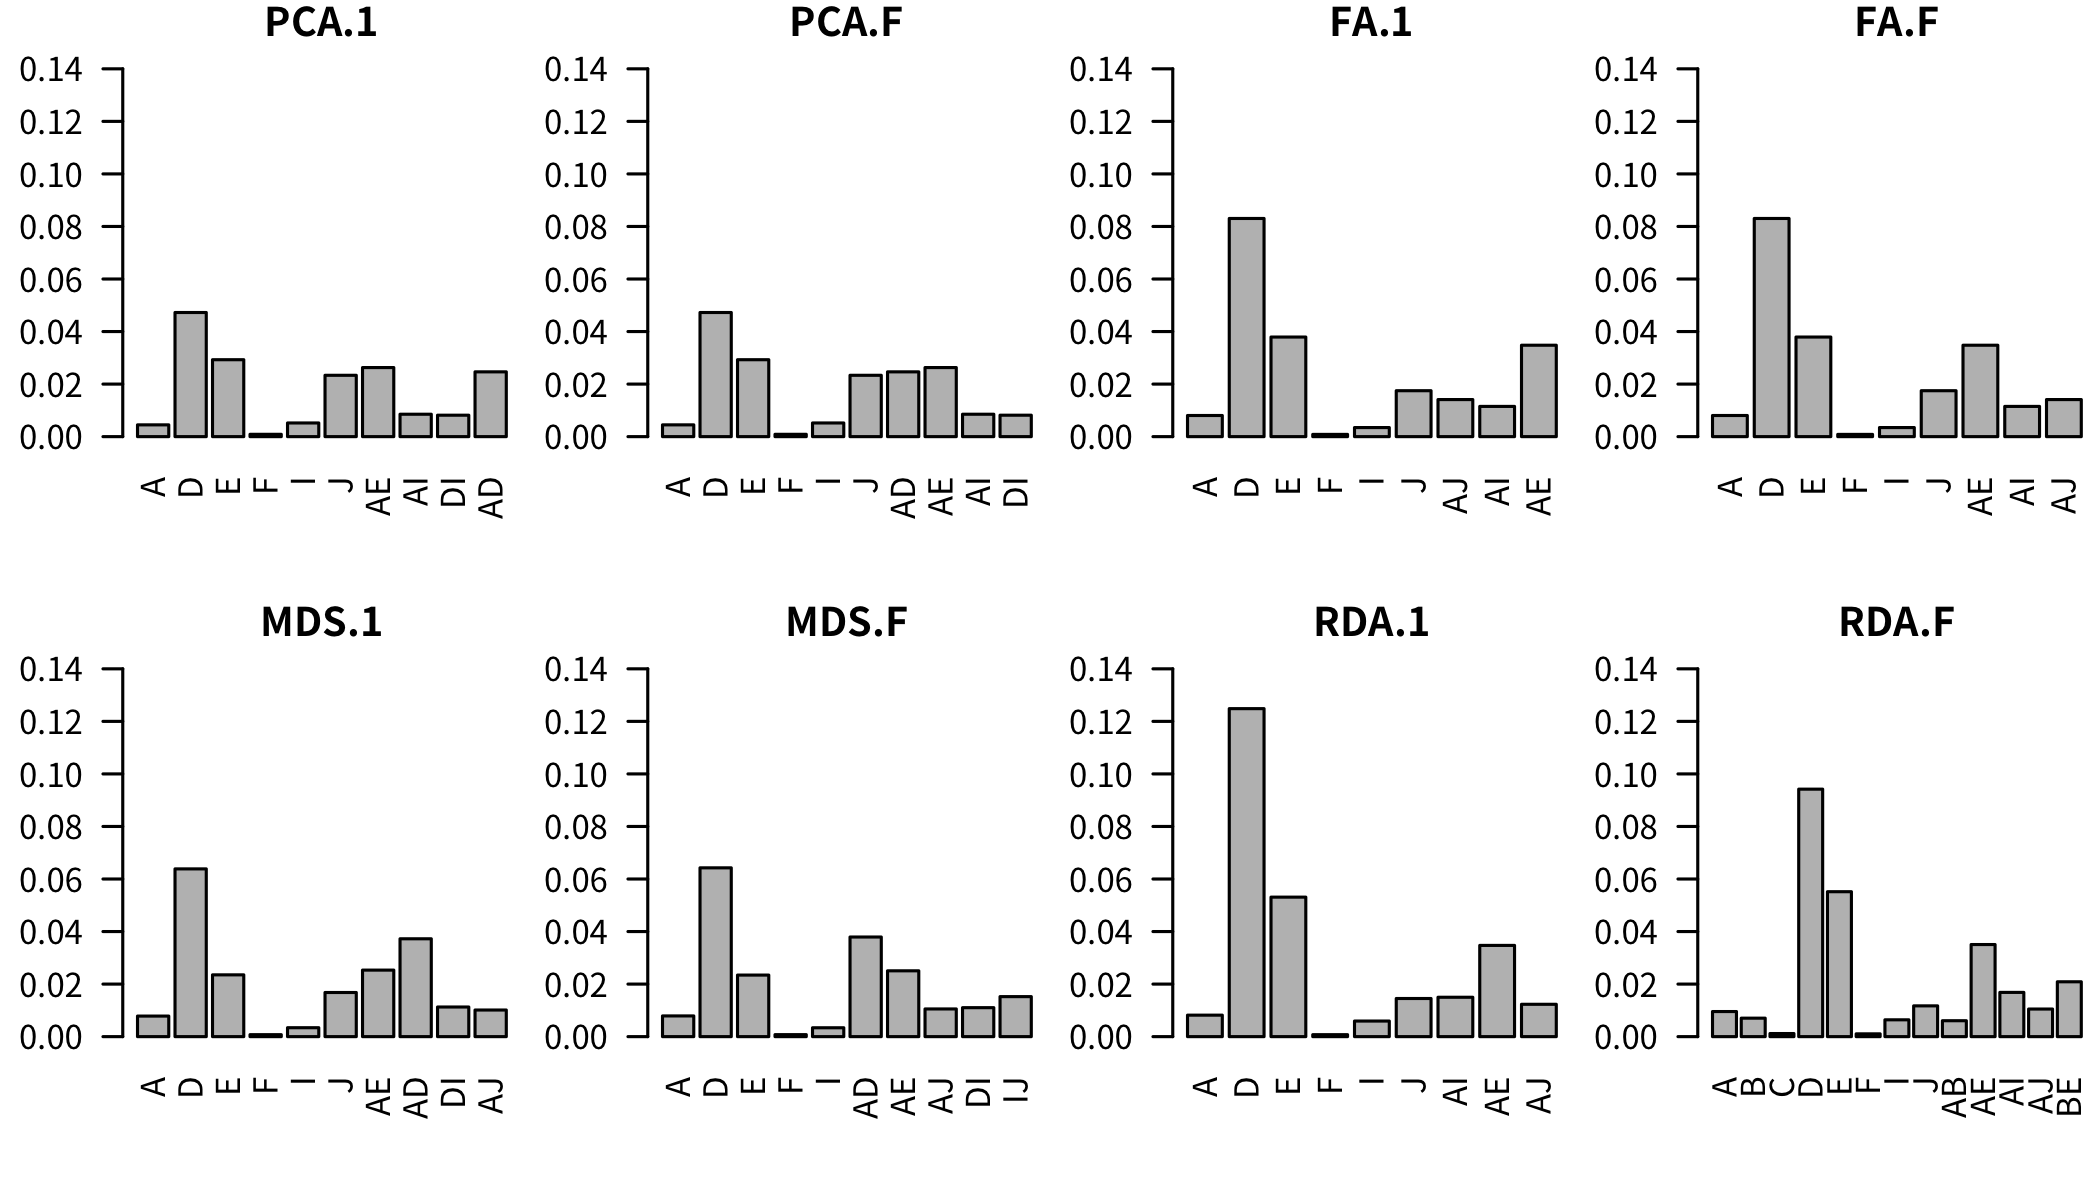
\includegraphics[width=1\textwidth]{beta相對貢獻量.png}
\end{frame}

\section{評價不同侯選TBAF構造分數}


\begin{frame}{生態分數的預測值與實際值的相關性}
\begin{columns}[onlytextwidth, c]
	\begin{column}{0.55\textwidth}
		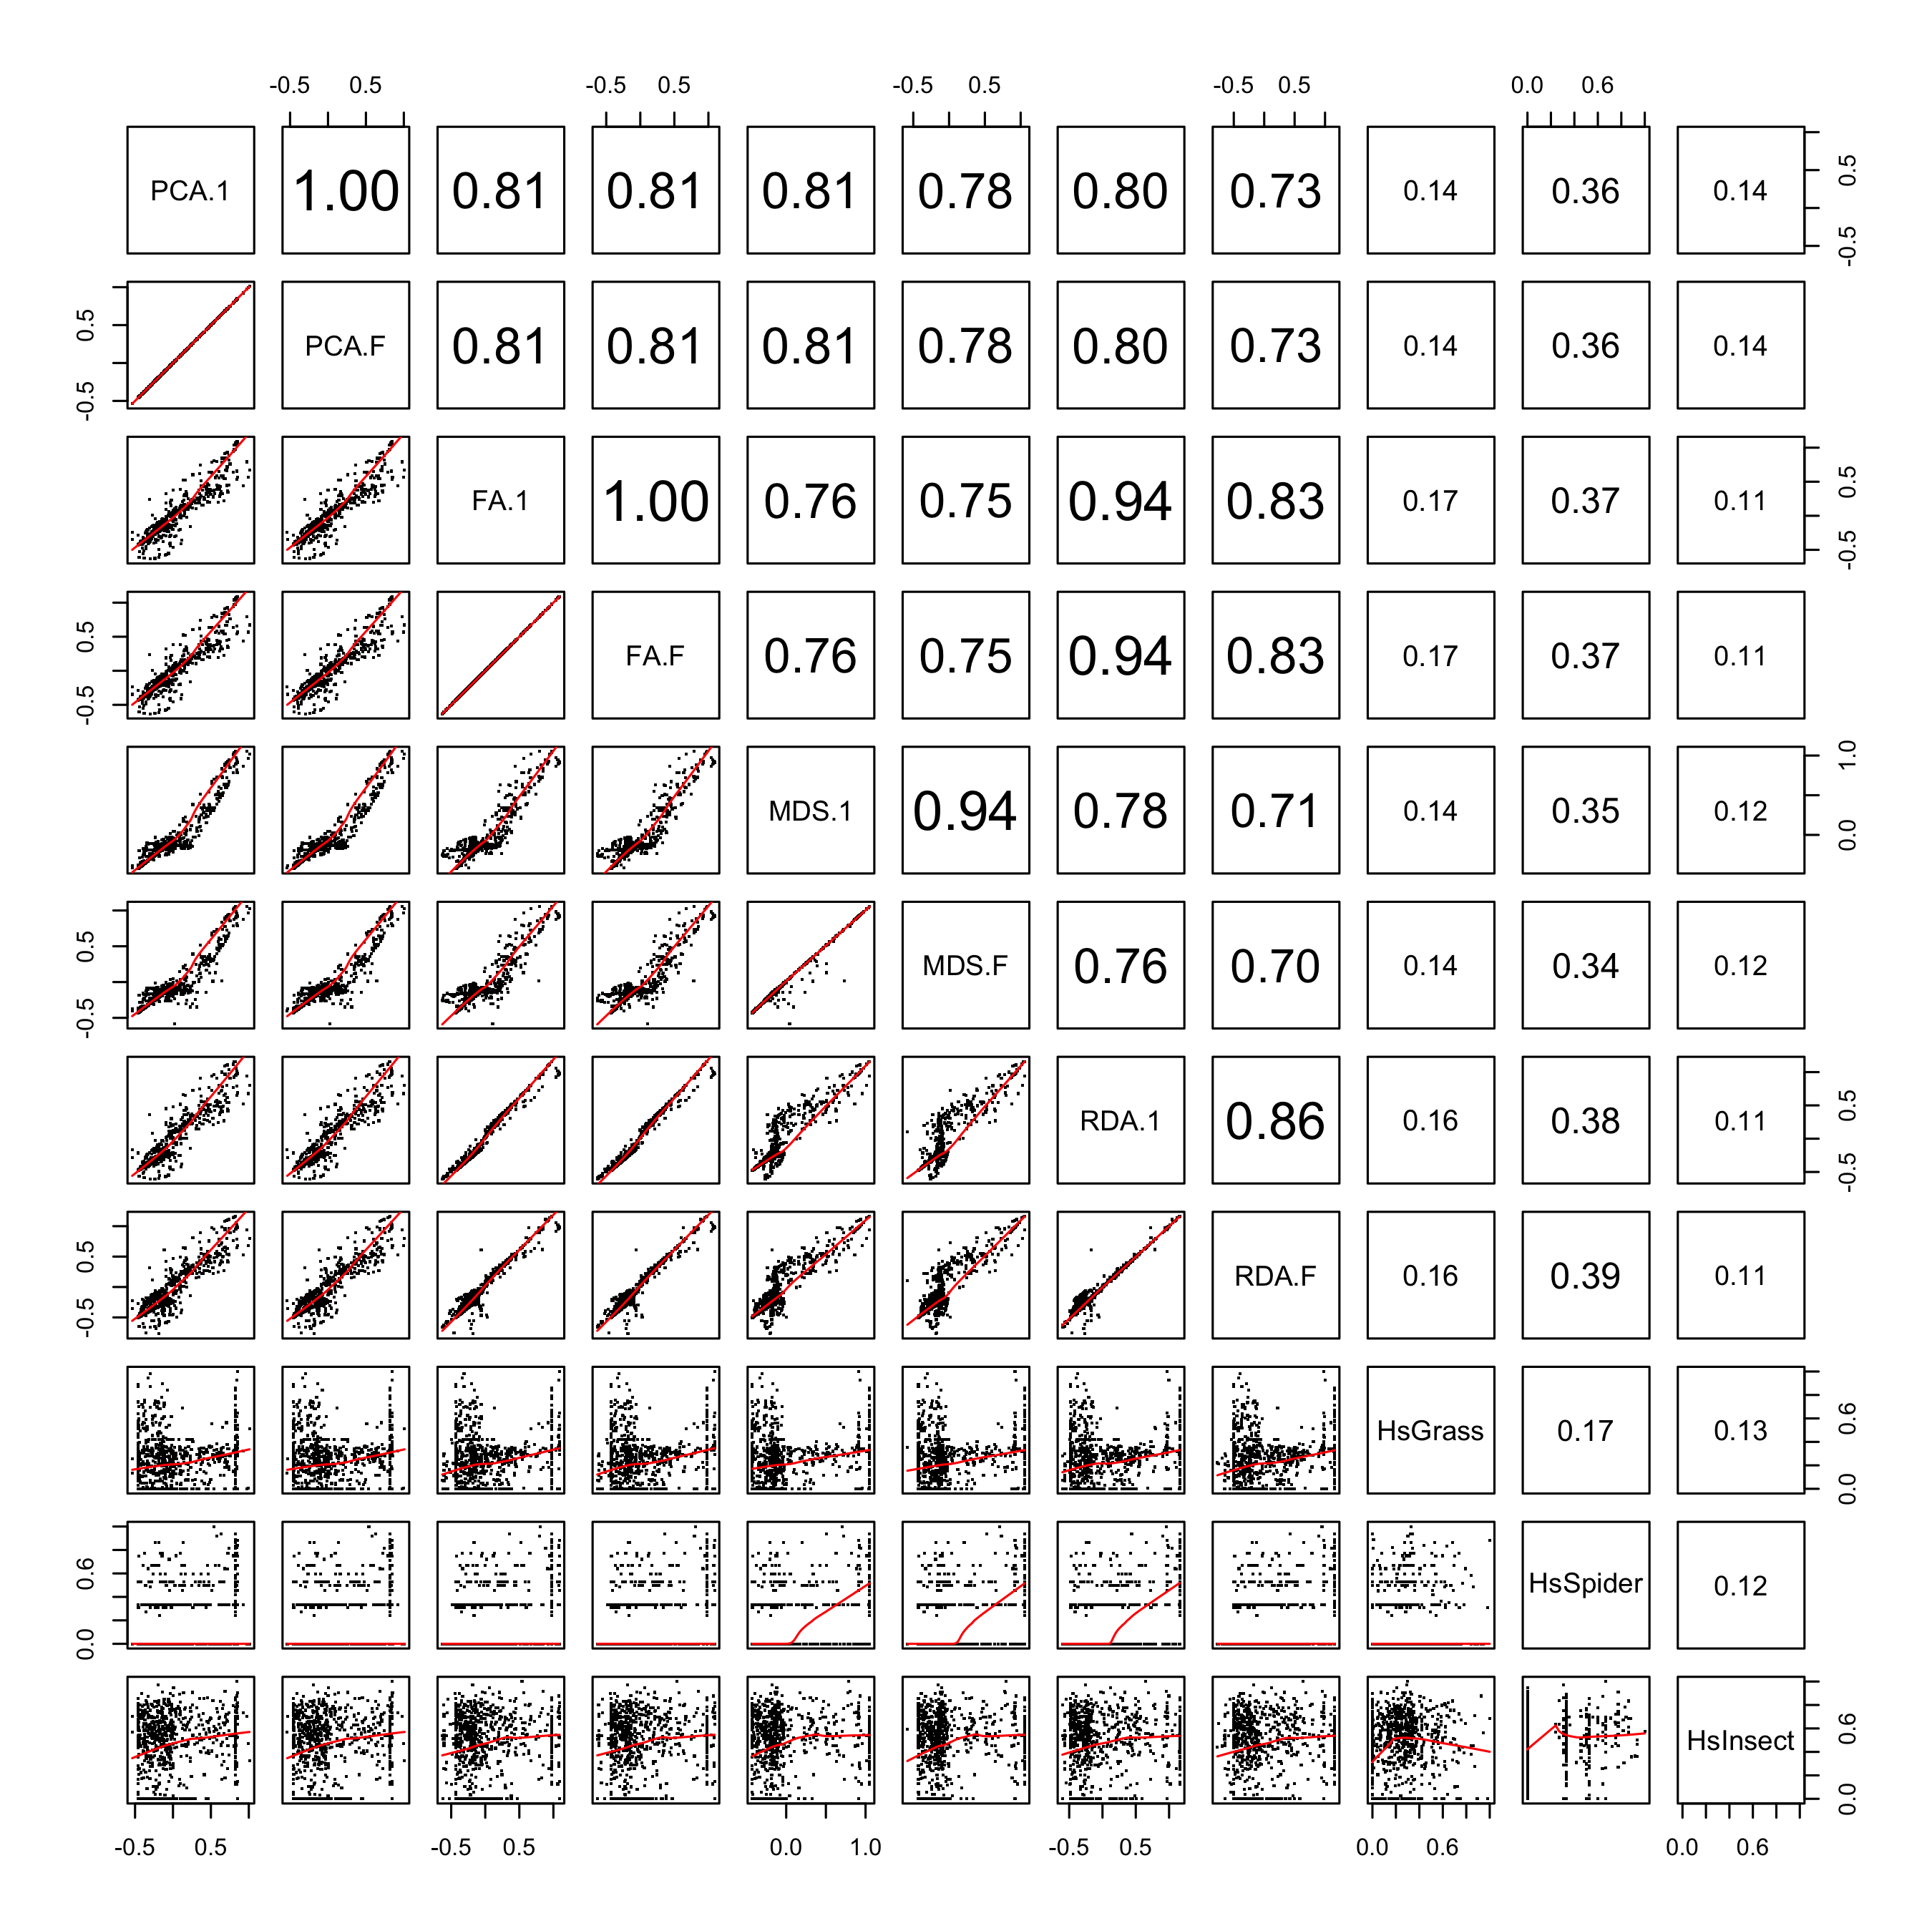
\includegraphics[trim=100 100 100 100, height=8cm]{all.png}
	\end{column}
	\begin{column}{0.45\textwidth}
		\begin{itemize}
			\item 8種模型對蜘蛛多樣性指數的預測能力最好,但也在Kendall rank correlation coefficient = 0.37左右
			\item 8種模型的效果似乎十分相似
		\end{itemize}
	\end{column}
\end{columns}
\end{frame}


\begin{frame}{侯選模型之預測能力}
% latex table generated in R 3.2.2 by xtable 1.8-0 package
% Wed Nov 18 06:06:24 2015
\begin{table}[ht]
\centering
{\small
\begin{mytabular}{lrrrrrrrr}
  \hline
 & PCA\textsubscript{1} & PCA\textsubscript{F} & FA\textsubscript{1} & FA\textsubscript{F} & MDS\textsubscript{1} & MDS\textsubscript{F} & RDA\textsubscript{1} & RDA\textsubscript{F} \\ 
  \hline
\# IV & 10.000 & 10.000 & 9.000 & 9.000 & 10.000 & 10.000 & 9.000 & 13.000 \\ 
  NRMSE & 0.906 & 0.906 & 0.888 & 0.888 & 0.894 & 0.894 & 0.854 & 0.851 \\ 
  $ R^2 $ & 0.178 & 0.178 & 0.211 & 0.211 & 0.200 & 0.199 & 0.269 & 0.276 \\ 
  Adjusted $ R^2 $ & 0.168 & 0.168 & 0.202 & 0.202 & 0.190 & 0.189 & 0.261 & 0.264 \\ 
  Kendall tau & 0.278 & 0.278 & 0.303 & 0.303 & 0.272 & 0.270 & 0.335 & 0.339 \\ 
  AIC/1000 & 2.118 & 2.118 & 2.083 & 2.083 & 2.096 & 2.097 & 2.023 & 2.024 \\ 
  BIC/1000 & 2.174 & 2.174 & 2.135 & 2.135 & 2.152 & 2.153 & 2.074 & 2.094 \\ 
   \hline
\end{mytabular}
}
\end{table}

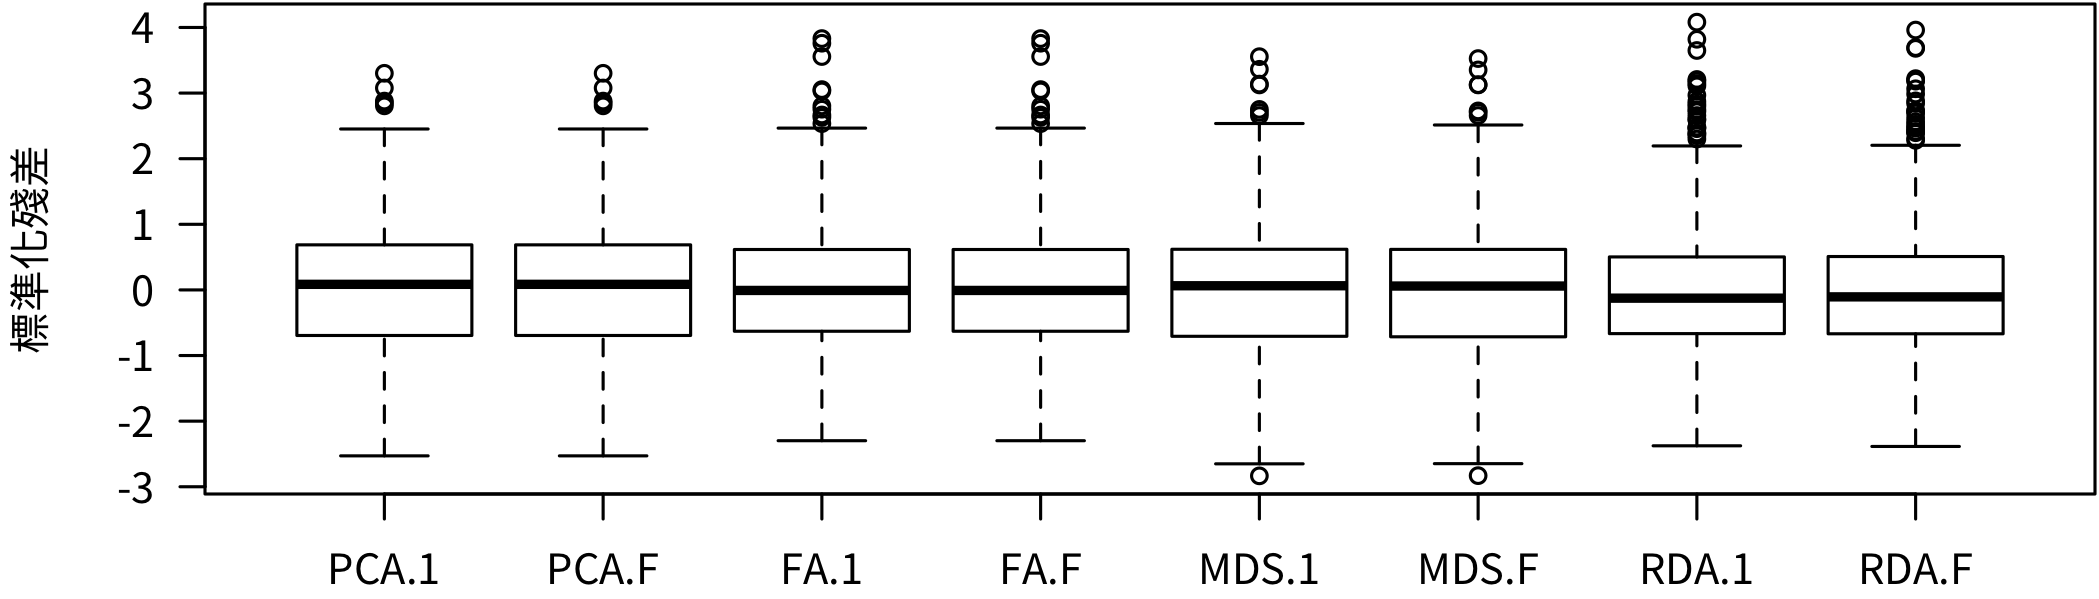
\includegraphics[width=1\textwidth]{resid最佳迴歸法.png}
\end{frame}


\begin{frame}{十折交插驗證}
\begin{enumerate}
	\item 將資料分10等份,其中9份為\alert{訓練資料集},另1份為\alert{驗證資料集}
	\item 以訓練資料集DV與IV建模$M$
	\item 以驗證資料集IV丟入模型$M$取得訓練資料集的預測結果
	\item 重覆2--3步驟10次,使所有資料都被驗證1次,取得所有預測結果$\hat{y}$
	\item 驗證資料集DV為$y$,求 normalized root-mean-square error(NRMSE)
		\[ \left. \sqrt{\frac{\sum_{t=1}^n (\hat y_t - y)^2}{n}} \middle/ \mathrm{SD}(y) \right. \]
	若$\mathrm{NRMSE} = 1$表示預測值與驗證值的差之幾何平均佔1個$y$的標準偏差
\end{enumerate}
\end{frame}


%
\begin{frame}{驗證迴歸及自動化變數挑選方法}
%\begin{description}
%	\item [目標] 比較不同迴歸及自動化變數挑選方法(AIC/BIC)
%	\item [訓練資料集] 預先降維之生態分數對面積資料進行複迴歸並自動迴歸式最佳化後,以驗證資料集之面積資料進行預測
%	\item [驗證資料集] 預先降維生態分數
%\end{description}
\centering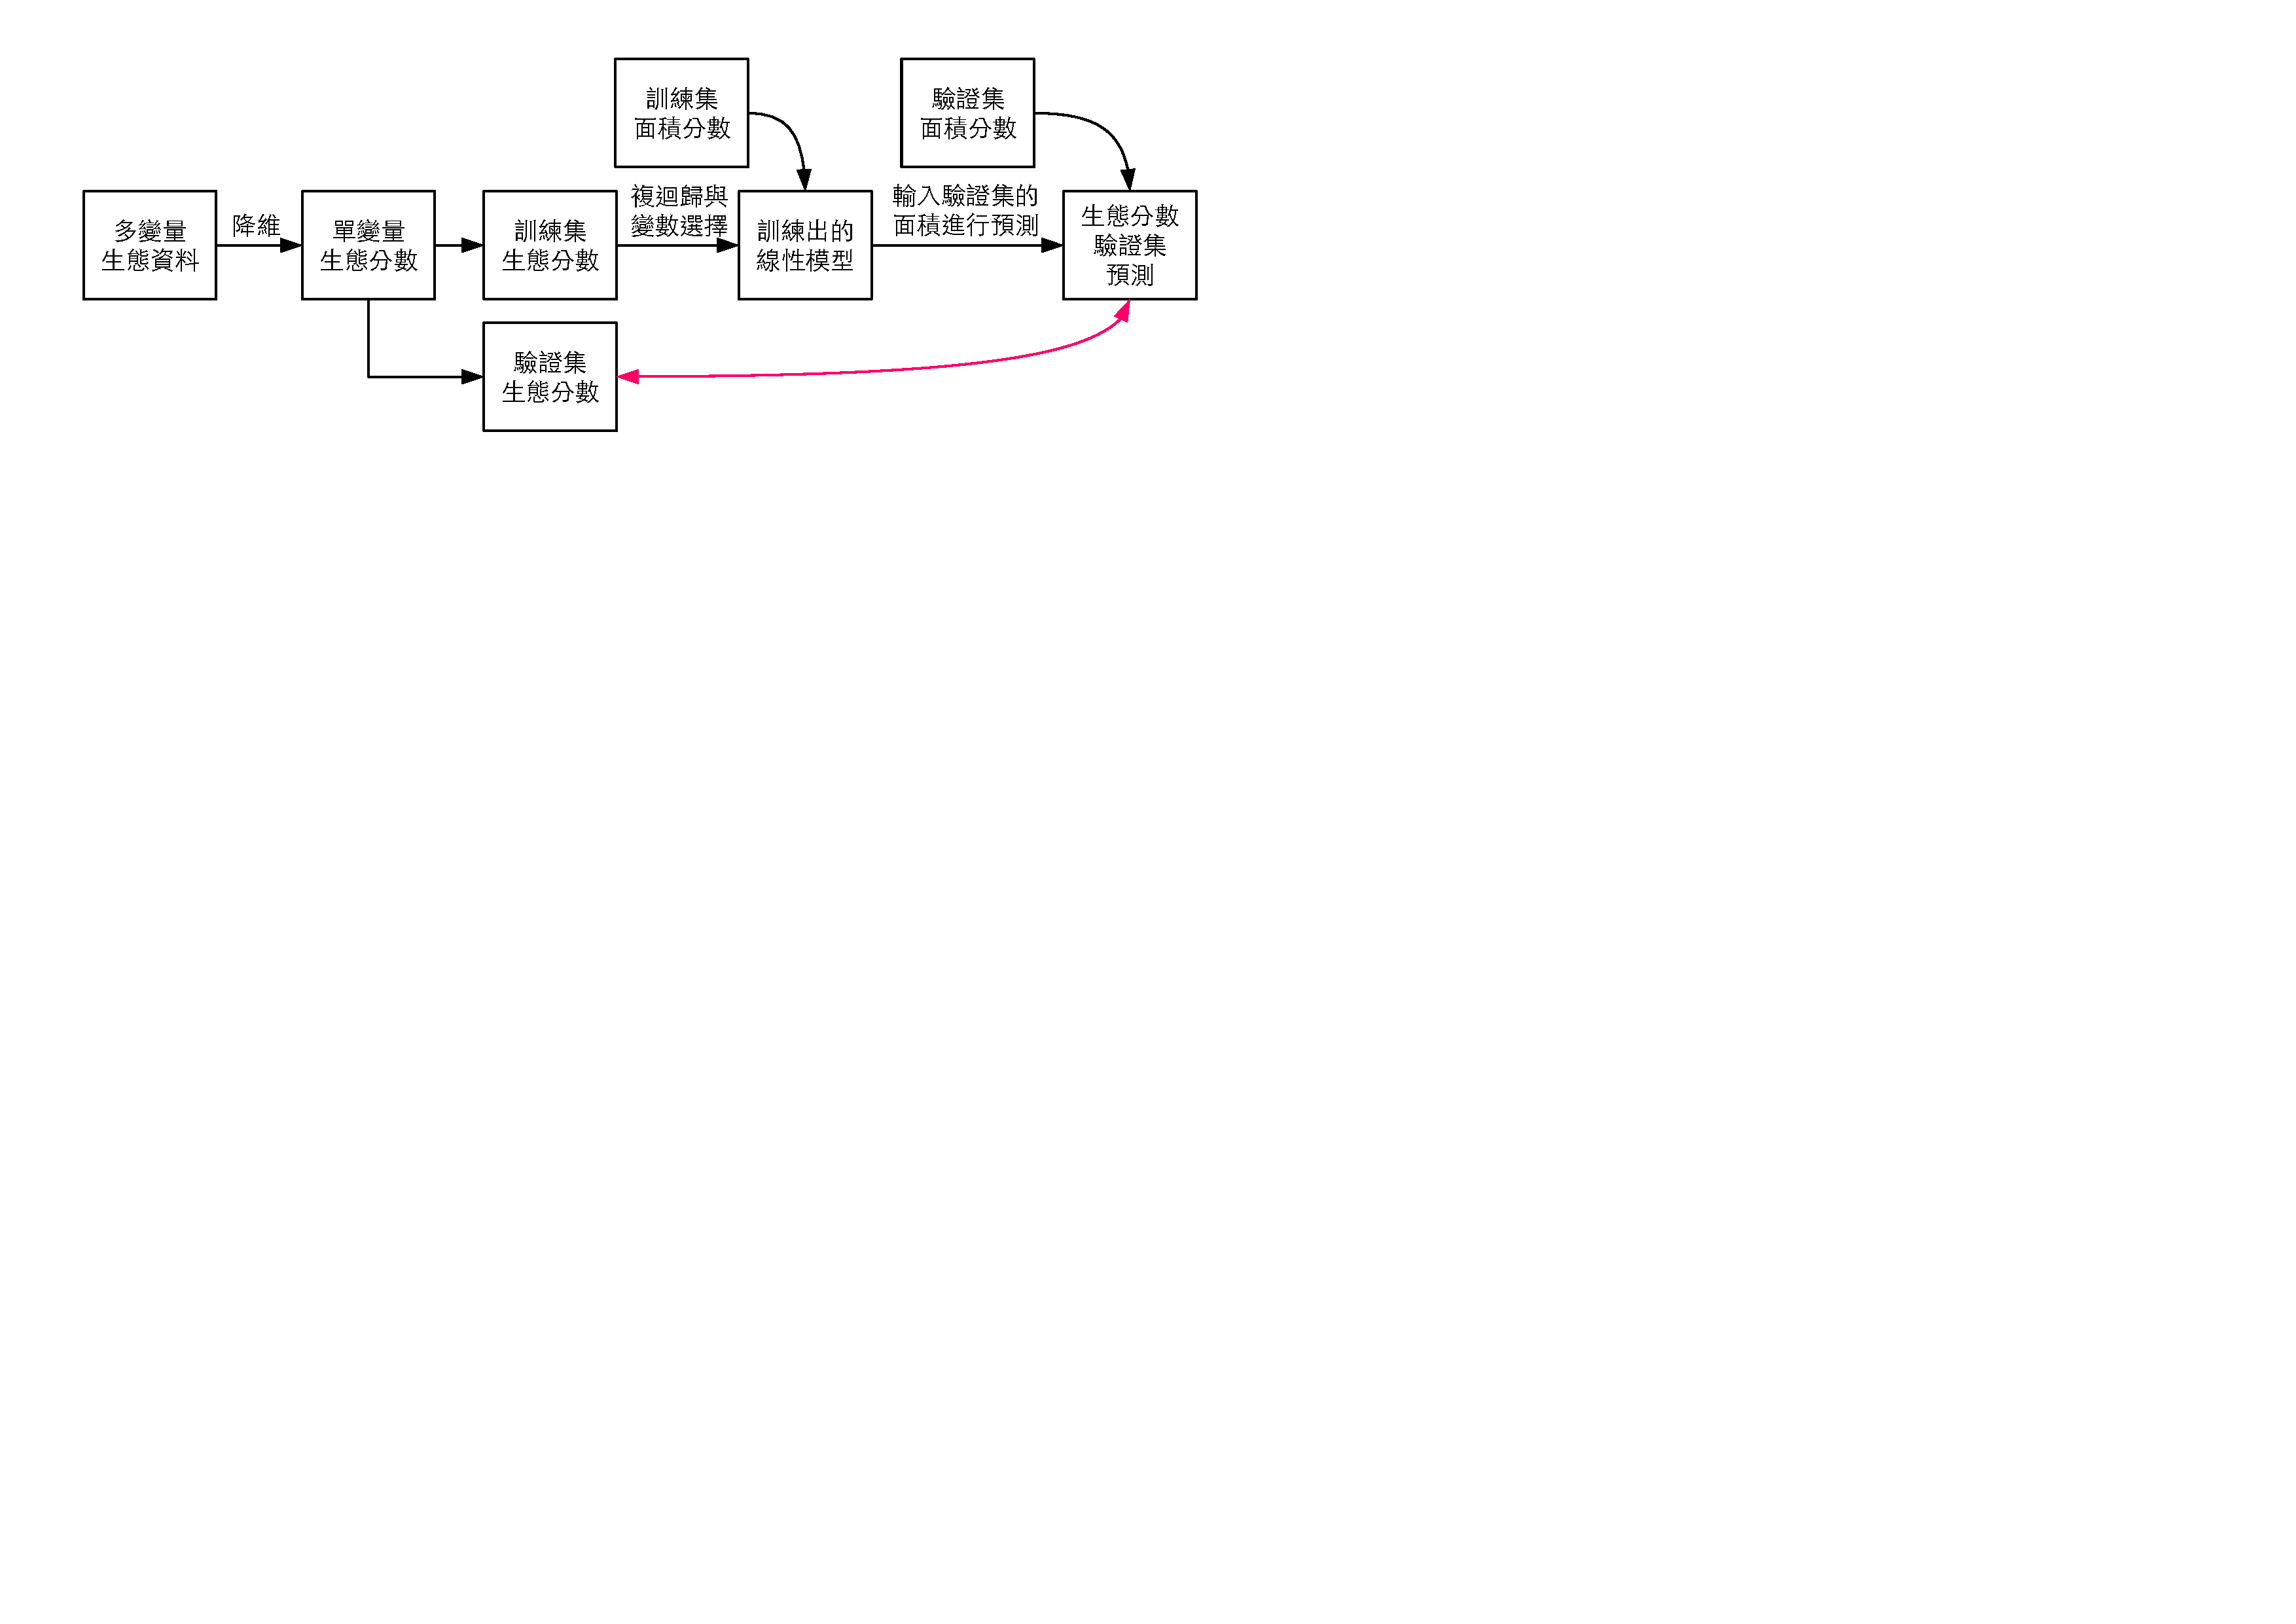
\includegraphics[width=1\textwidth]{diagram-驗證迴歸及自動化變數挑選方法.pdf}
% latex table generated in R 3.2.2 by xtable 1.8-0 package
% Wed Nov 18 06:07:03 2015
\begin{table}[ht]
\centering
{\normalsize
\begin{mytabular}{lrrrrrrrr}
  \hline
 & PCA\textsubscript{1} & PCA\textsubscript{F} & FA\textsubscript{1} & FA\textsubscript{F} & MDS\textsubscript{1} & MDS\textsubscript{F} & RDA\textsubscript{1} & RDA\textsubscript{F} \\ 
  \hline
NRMSE & 0.929 & 0.929 & 0.902 & 0.904 & 0.918 & 0.922 & 0.873 & 0.874 \\ 
  Pearson r & 0.375 & 0.374 & 0.431 & 0.428 & 0.400 & 0.393 & 0.489 & 0.488 \\ 
  Kendall tau & 0.236 & 0.235 & 0.267 & 0.262 & 0.225 & 0.216 & 0.297 & 0.297 \\ 
   \hline
\end{mytabular}
}
\end{table}

%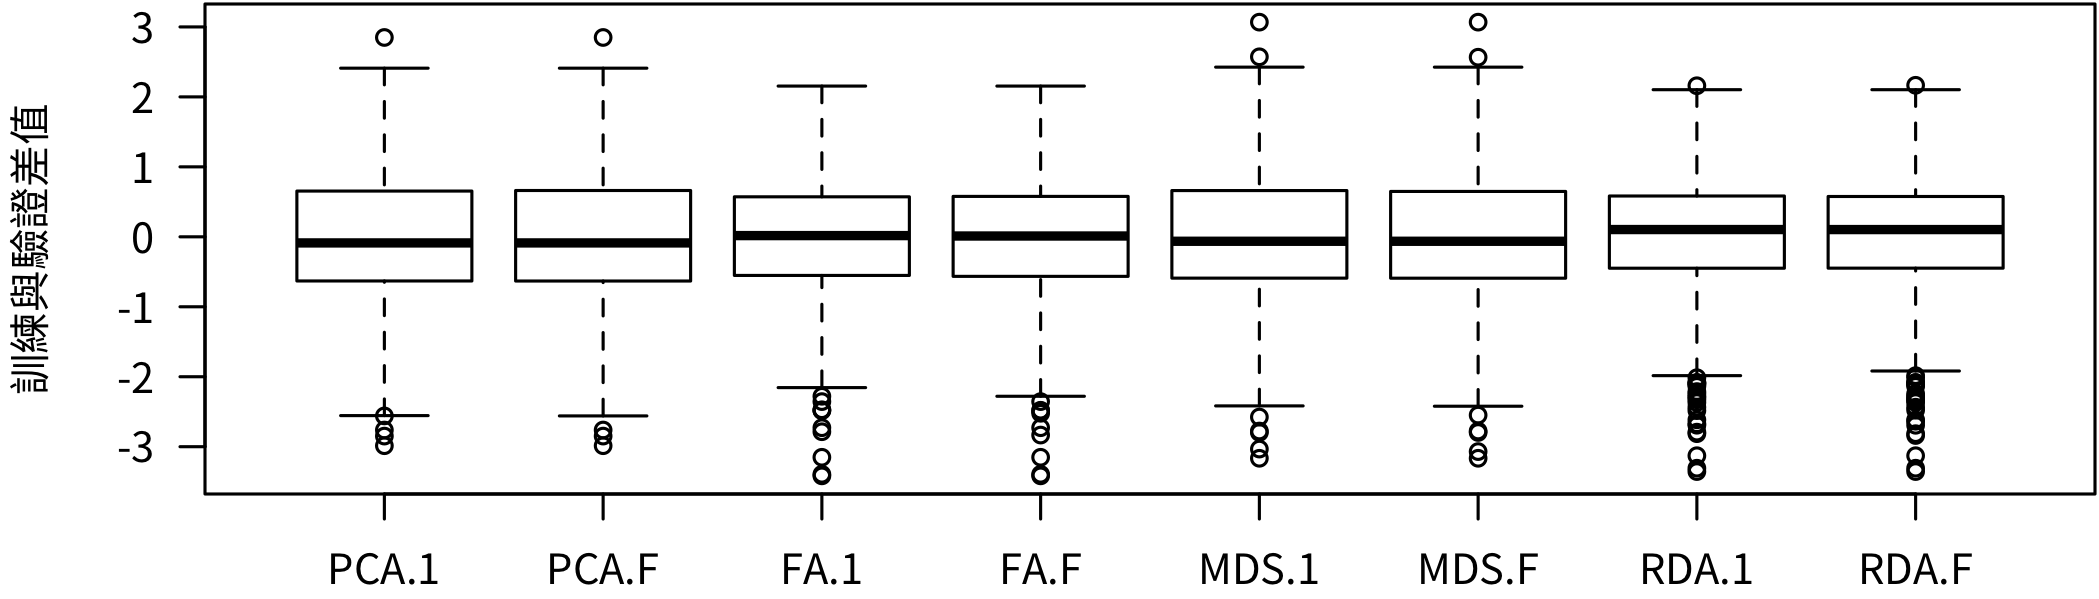
\includegraphics[width=1\textwidth]{CV求最佳迴歸法.png}
\end{frame}


\begin{frame}{驗證面積資料變數組合}
%\begin{description}
%	\item [目標] 比較哪組面積變數組合較佳
%	\item [訓練資料集] 預先降維的生態分數,對所有對應之面積資料對預先取得的面積變數組合(只是組合,不包括迴歸係數)進行複迴歸後,以驗證資料集之面積資料進行預測
%	\item [驗證資料集] 預先降維後的生態分數
%\end{description}
\centering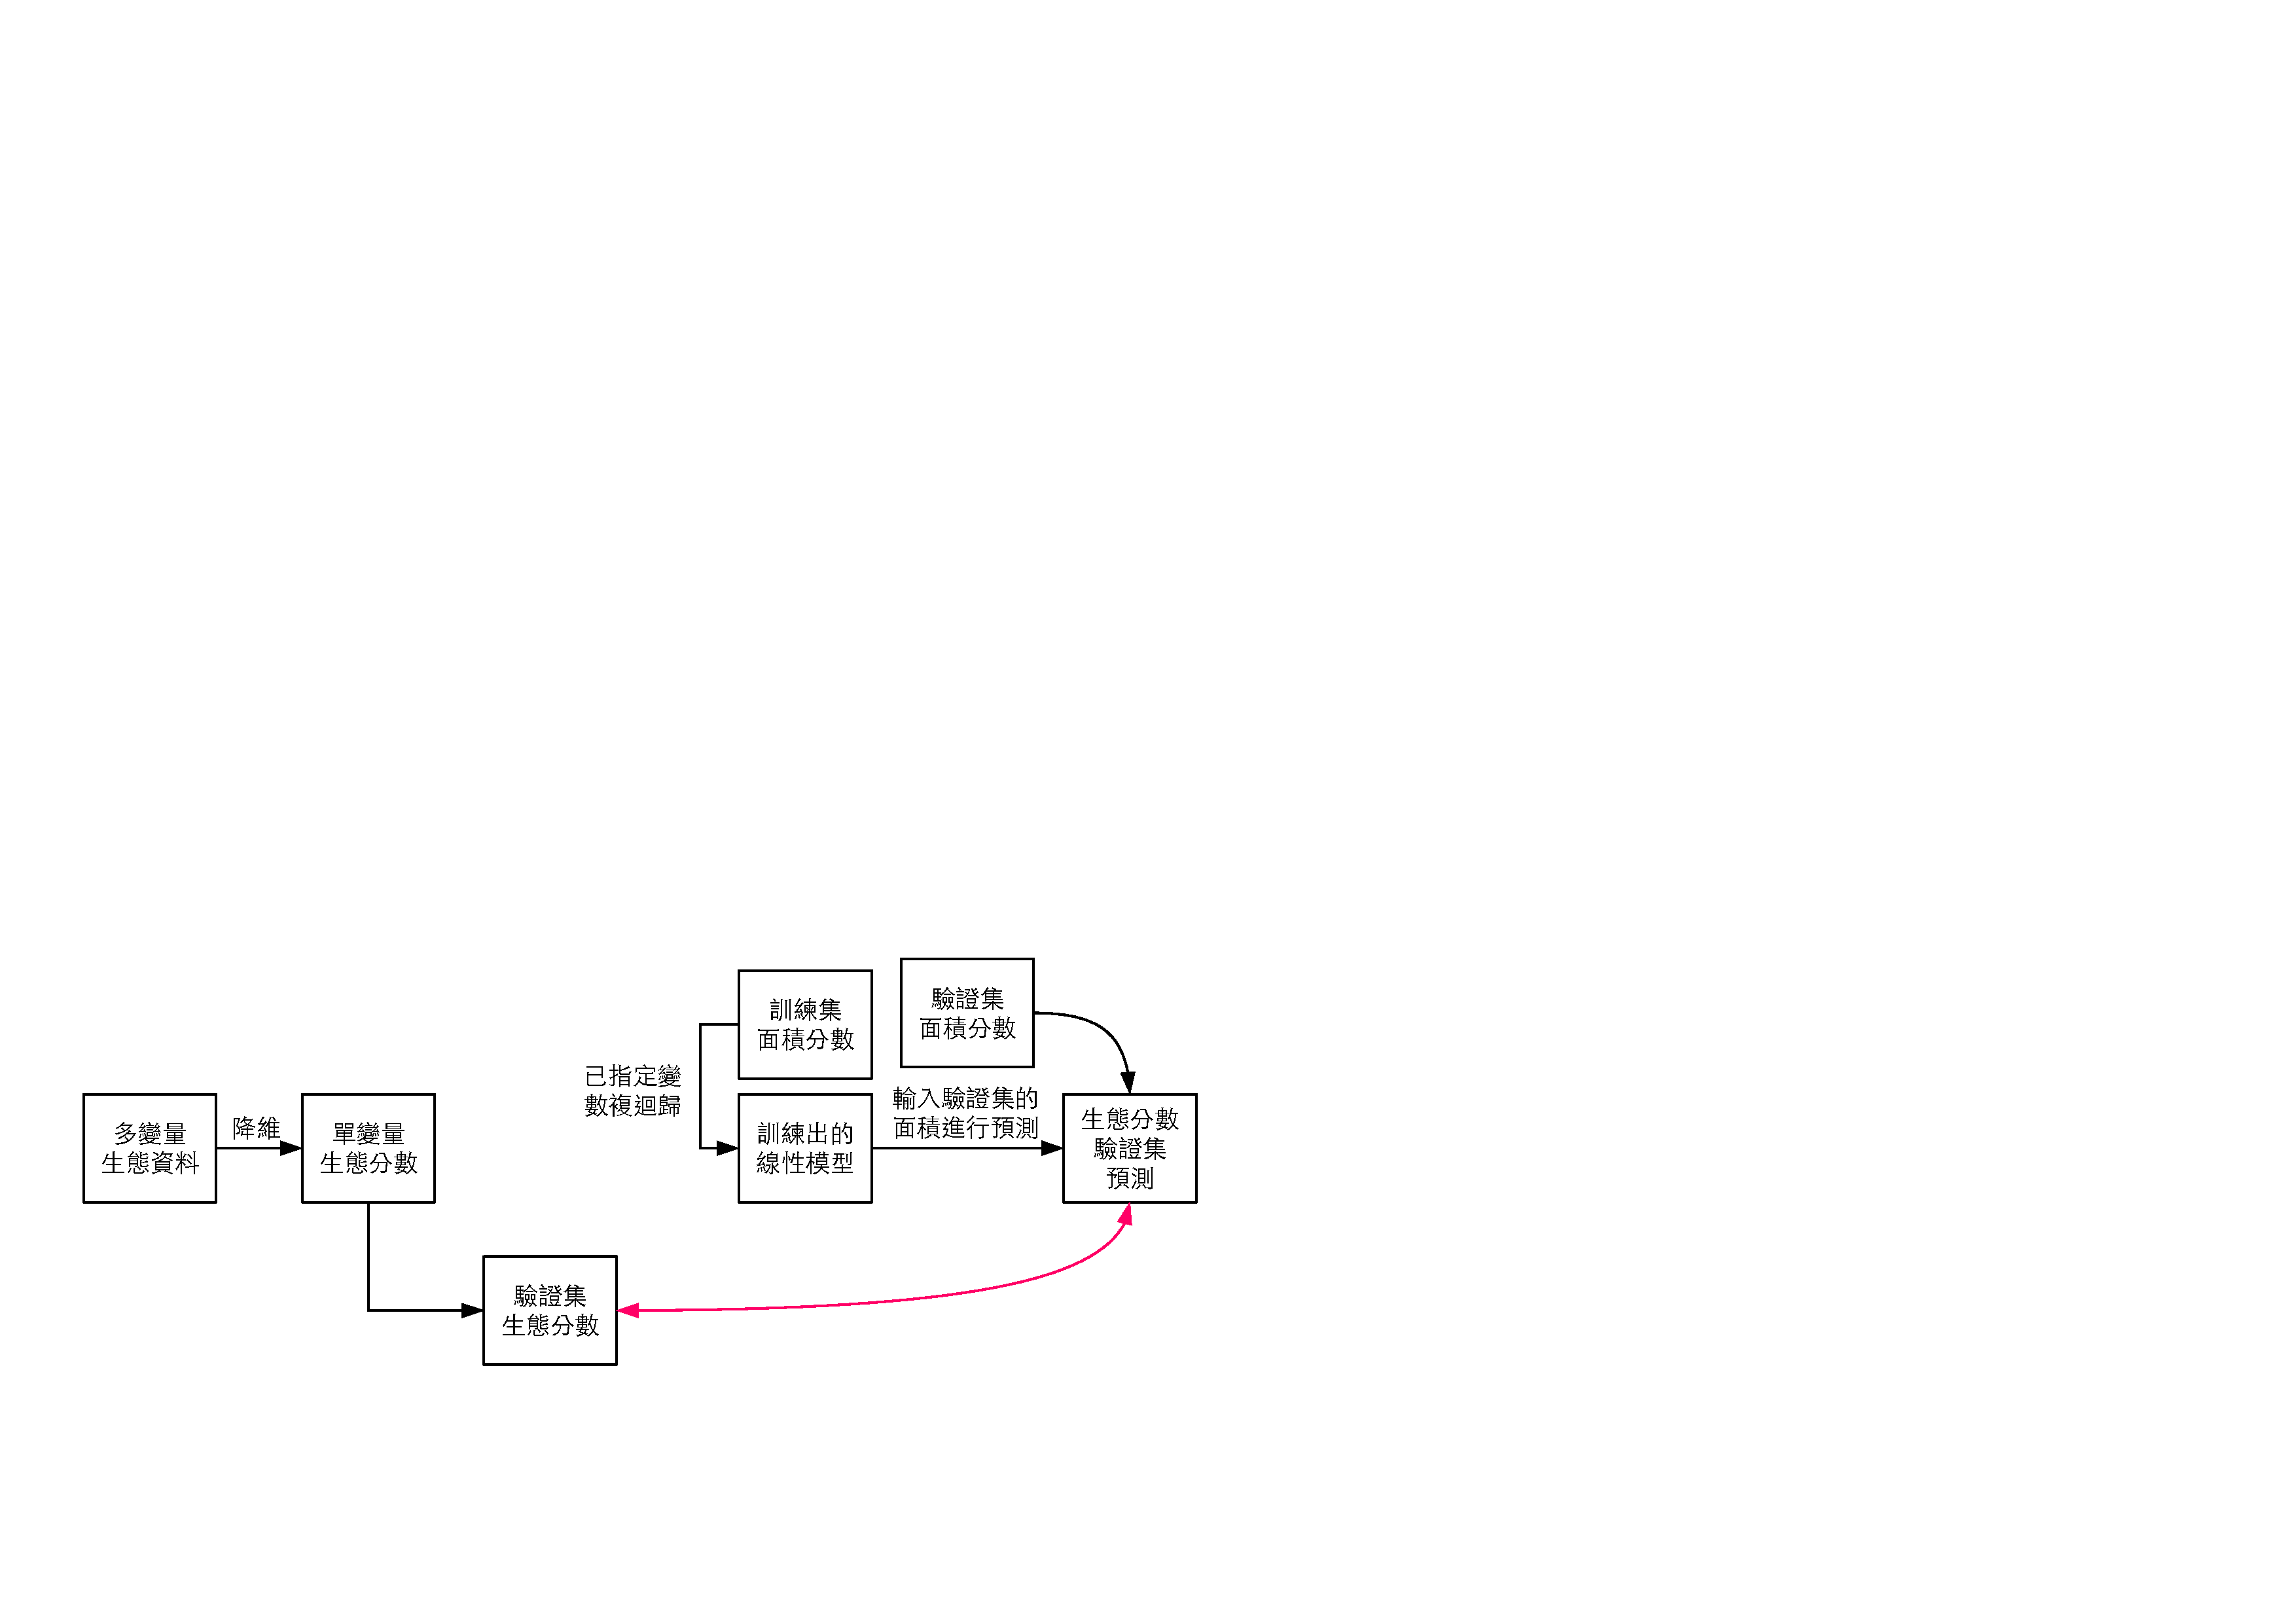
\includegraphics[width=1\textwidth]{diagram-驗證面積資料變數組合.pdf}
% latex table generated in R 3.2.2 by xtable 1.8-0 package
% Wed Nov 18 06:07:06 2015
\begin{table}[ht]
\centering
{\normalsize
\begin{mytabular}{lrrrrrrrr}
  \hline
 & PCA\textsubscript{1} & PCA\textsubscript{F} & FA\textsubscript{1} & FA\textsubscript{F} & MDS\textsubscript{1} & MDS\textsubscript{F} & RDA\textsubscript{1} & RDA\textsubscript{F} \\ 
  \hline
NRMSE & 0.924 & 0.923 & 0.902 & 0.902 & 0.911 & 0.908 & 0.867 & 0.868 \\ 
  Pearson r & 0.382 & 0.385 & 0.432 & 0.431 & 0.412 & 0.420 & 0.498 & 0.497 \\ 
  Kendall tau & 0.240 & 0.242 & 0.269 & 0.256 & 0.231 & 0.235 & 0.309 & 0.306 \\ 
   \hline
\end{mytabular}
}
\end{table}

%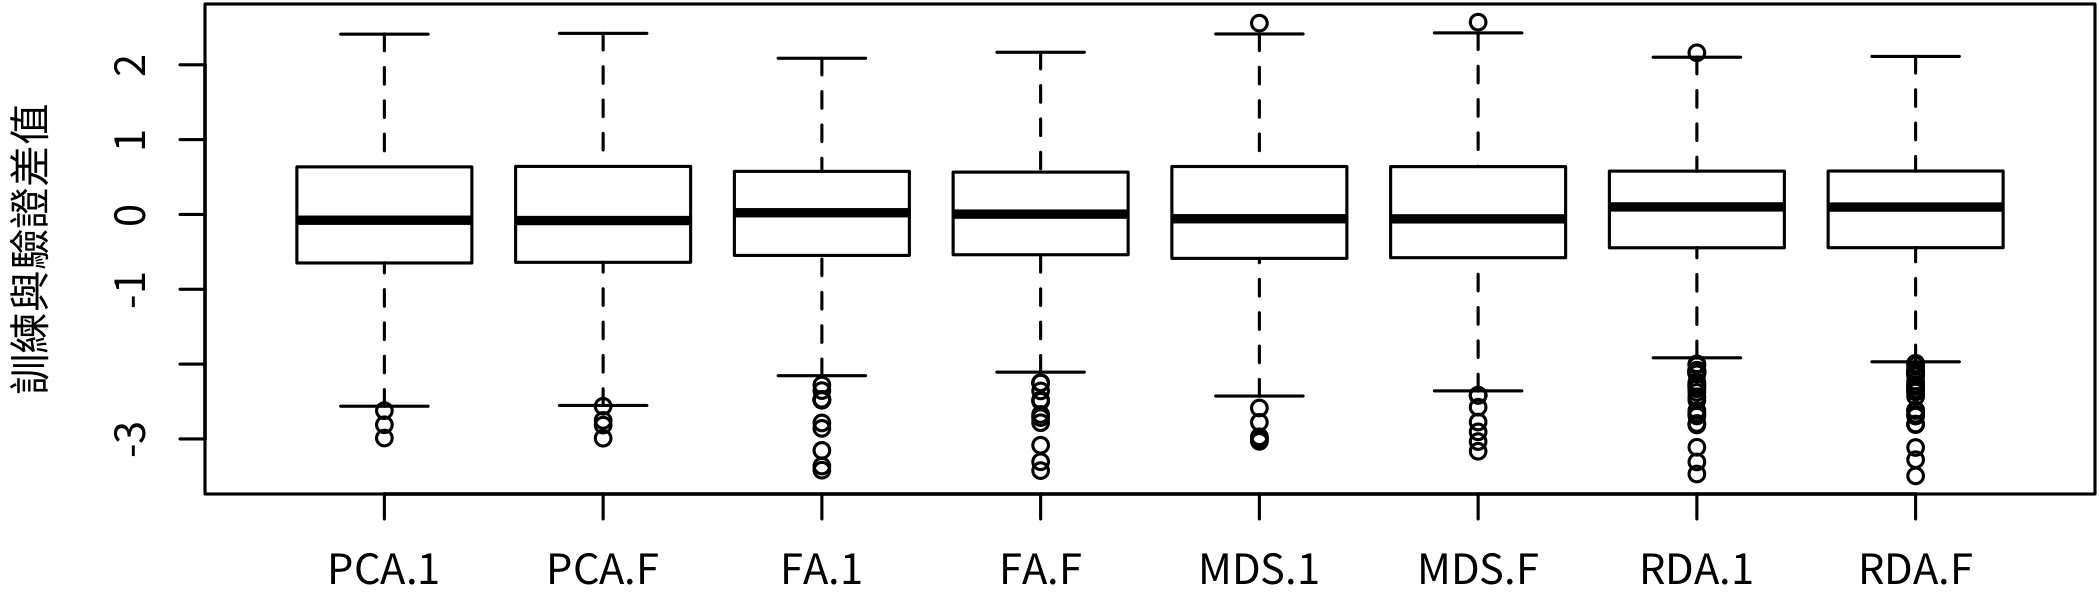
\includegraphics[width=1\textwidth]{CV-最佳解釋變數組.png}
\end{frame}





\begin{frame}{綜合比較不同求解方式}
%\begin{description}
%	\item [目標] 尋求較佳建模方式,包括降維與迴歸式最佳化
%	\item [訓練資料集] 獨立降維後的生態分數,對所有對應之面積資料進行複迴歸並自動迴歸式最佳化後,以驗證資料集之面積資料進行預測
%	\item [驗證資料集] 獨立降維後的生態分數
%\end{description}
\centering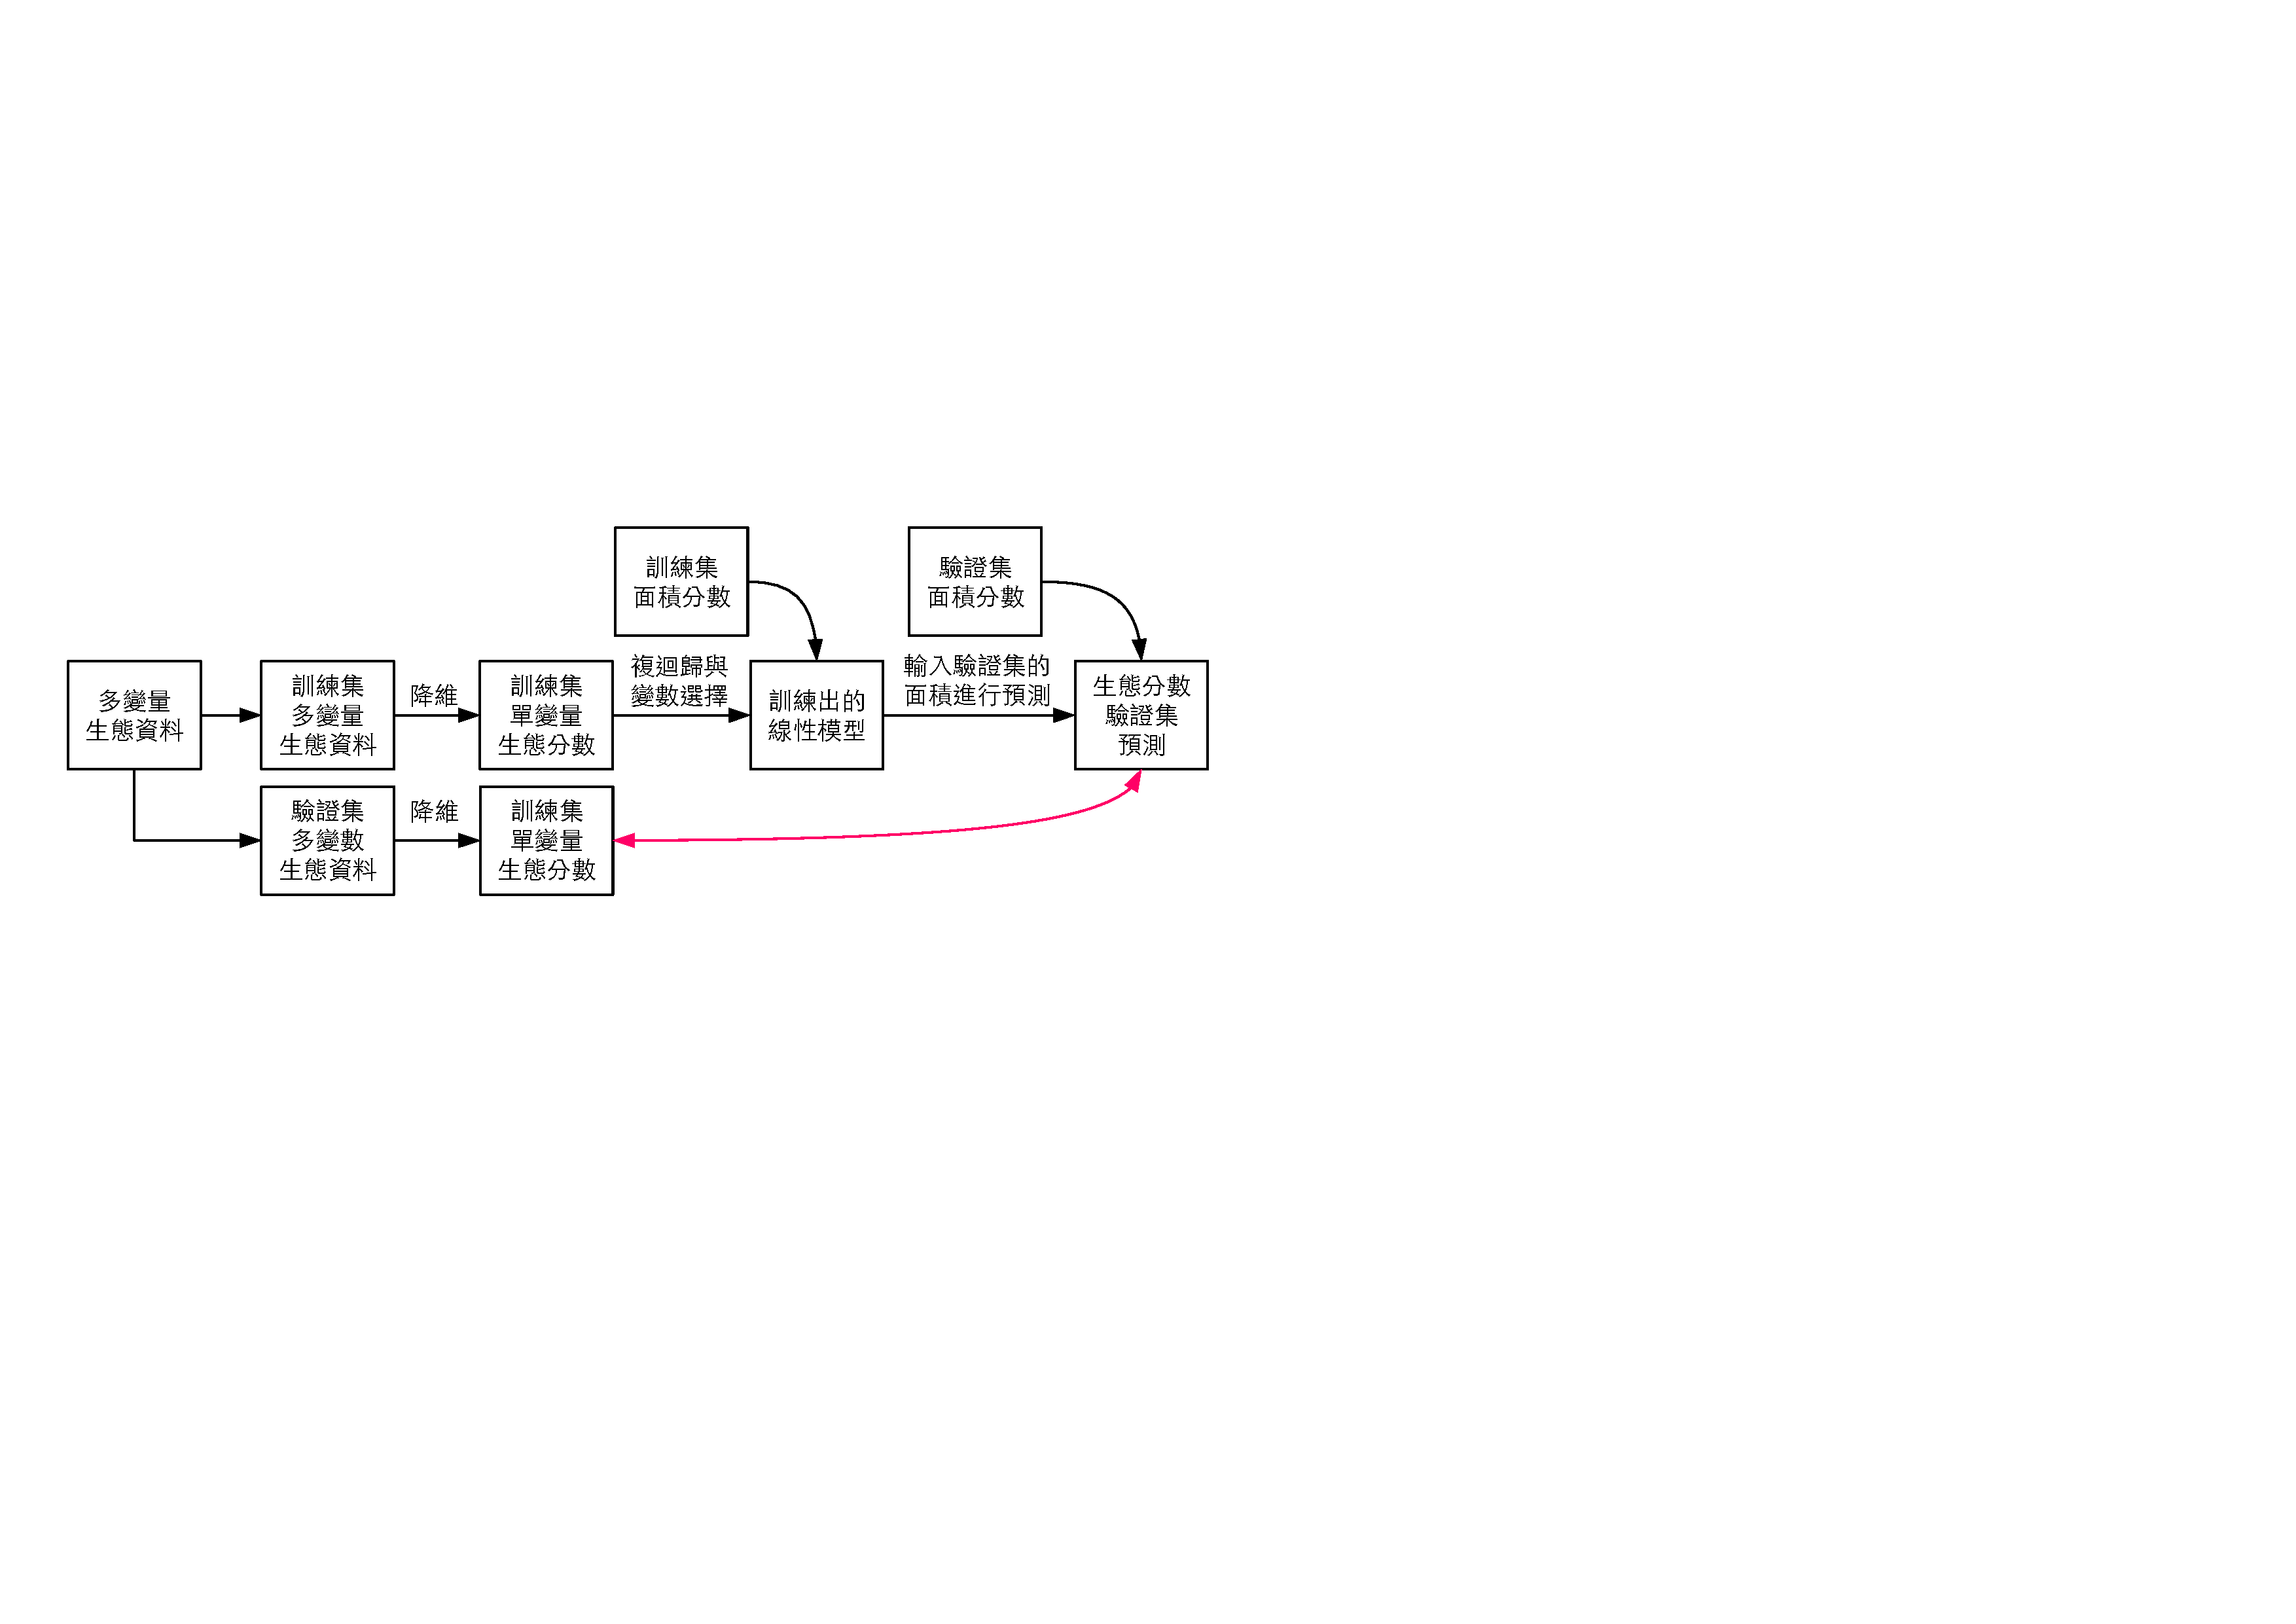
\includegraphics[width=1\textwidth]{diagram-綜合比較不同求解方式.pdf}
% latex table generated in R 3.2.2 by xtable 1.8-0 package
% Wed Nov 18 06:16:13 2015
\begin{table}[ht]
\centering
{\normalsize
\begin{mytabular}{lrrrrrrrr}
  \hline
 & PCA\textsubscript{1} & PCA\textsubscript{F} & FA\textsubscript{1} & FA\textsubscript{F} & MDS\textsubscript{1} & MDS\textsubscript{F} & RDA\textsubscript{1} & RDA\textsubscript{F} \\ 
  \hline
NRMSE & 0.935 & 0.938 & 0.928 & 0.931 & 1.138 & 1.137 & 0.937 & 0.945 \\ 
  Pearson r & 0.361 & 0.356 & 0.380 & 0.378 & $-$0.094 & $-$0.088 & 0.378 & 0.368 \\ 
  Kendall tau & 0.224 & 0.222 & 0.233 & 0.232 & $-$0.048 & $-$0.046 & 0.227 & 0.218 \\ 
   \hline
\end{mytabular}
}
\end{table}

%\centering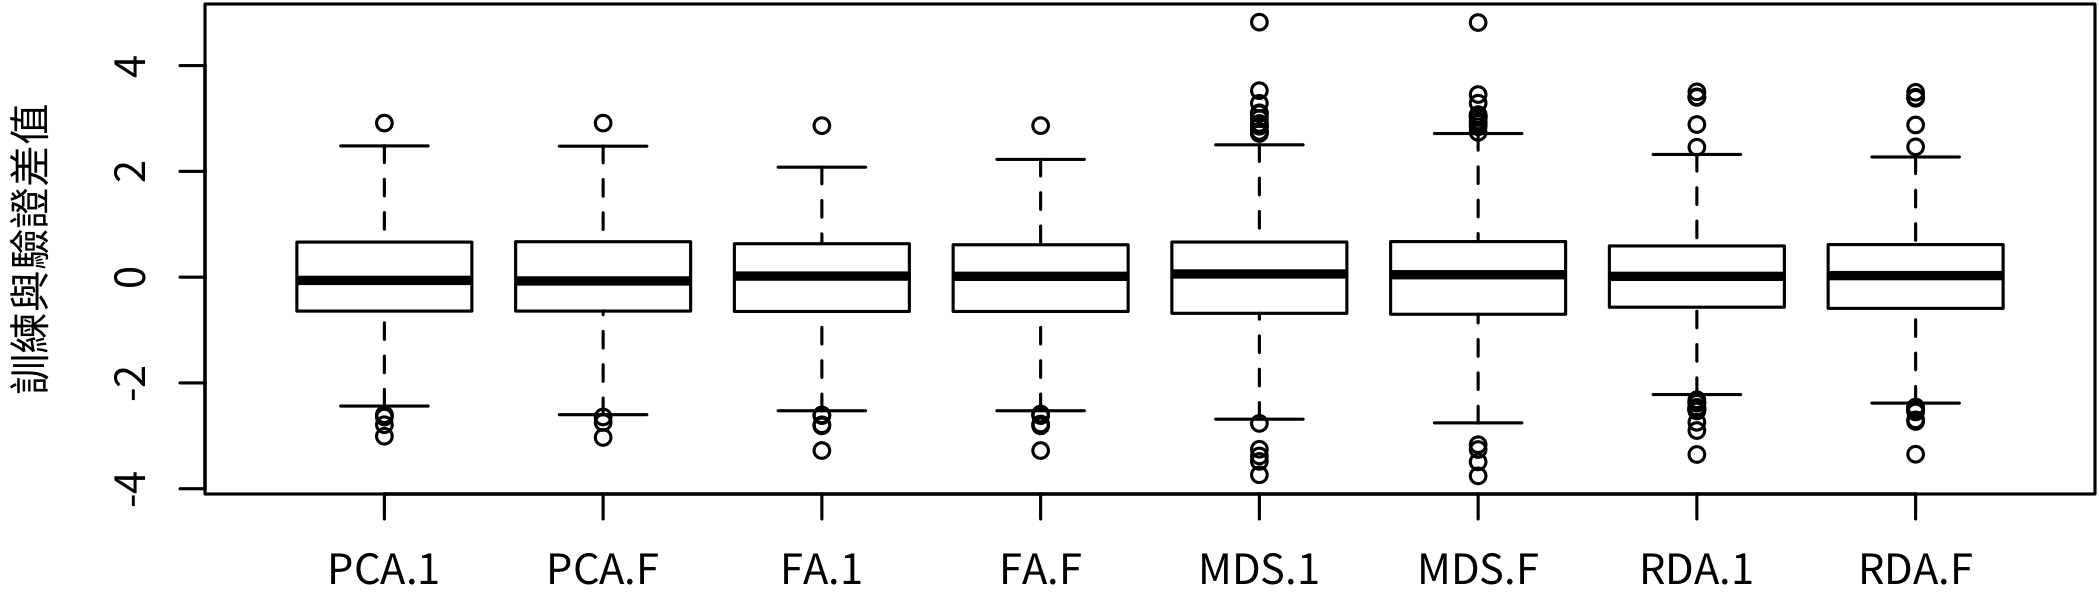
\includegraphics[width=1\textwidth]{CV-final.png}
\end{frame}



\begin{frame}{綜合比較結論}
\begin{itemize}
	\item PCA與RDA降維後,無論以AIC或BIC法,其預測值與實際生態資料的相關性較高且交叉驗證的誤差較低
	\item BIC的結果比AIC還精簡(留下的解釋變數少了約一半),且交叉驗證結果指出二者都沒有明顯過度配適(overfitting)問題
	\item RDA在降維時一併考慮了面積資料,但目前資料並不是非常全面性的;若以RDA結果為TBAF構造分數要更小心「以外插法求解往往是危險的」的情況
	\item MDS的特性是著重不相似性(概念上類似4種多樣性指數的組成比例在樣點間的差距)
	\item FA太過偏好昆蟲多樣性指數,且在每次訓練過程過度偏好訓練子集資料,驗證能力較差
	\item 不同的迴歸解釋變數組合以PCA與RDA驗證能力較佳,但其實二者並不是非常相似;原因可能是資料特性(共線性)或需配合專業知識辨別何者較合理
\end{itemize}
\end{frame}


\begin{frame}{目前我認為最好的TBAF建構係數組}
按目前結果,我認為RDA\textsubscript{AIC}的係數可以發展為TBAF建構分數。A--J的單位為比例(0--1)
% latex table generated in R 3.2.2 by xtable 1.8-0 package
% Wed Nov 18 02:31:15 2015
\begin{table}[ht]
\centering
{\normalsize
\begin{mytabular}{lrrrr}
  \hline
 & FA\textsubscript{1}已中心化 & RDA\textsubscript{1}已中心化 & FA\textsubscript{1}未中心化 & RDA\textsubscript{1}未中心化 \\
  \hline
Int. & 0.04972 & 0.04469 & -0.0594563053 & -0.1660450534\\
  $ A $ & 0.21781 & 0.34981 & -0.5471588221 & -0.3980290910\\
   $A \times E $ & 1.50333 & 1.21649 & 1.5033315634 & 1.2164858262 \\
   $A \times I $ & 2.45668 & 3.01409 & 2.4566805629 & 3.0140897708\\
   $A \times J $ & $-$2.16068 & $-$2.11685 & -2.1606755410 & -2.1168453546\\
  $ D $ & 1.03635 & 1.32543 & 1.0363492651 & 1.3254339384\\
  $ E $ & $-$0.09021 & $-$0.08447 & -0.3719367565 & -0.3124394208\\
  $ F $ & $-$0.18668 & 0.07723 & -0.1866814866 & 0.0772270472\\
  $ I $ & 0.31146 & 0.49309 & -0.1489308375 & -0.0717603507 \\
  $ J $ & 0.74532 & 0.74315 & 1.1502336883 & 1.1398493291\\
   \hline
\end{mytabular}
}
\end{table}
%% latex table generated in R 3.2.2 by xtable 1.8-0 package
% Wed Nov 18 06:16:14 2015
\begin{table}[ht]
\centering
{\normalsize
\begin{mytabular}{lrr}
  \hline
 & FA\textsubscript{1} & RDA\textsubscript{1} \\ 
  \hline
Int. & 0.04972 & 0.04469 \\ 
  $ A $ & 0.21781 & 0.34981 \\ 
   $A \times E $ & 1.50333 & 1.21649 \\ 
   $A \times I $ & 2.45668 & 3.01409 \\ 
   $A \times J $ & $-$2.16068 & $-$2.11685 \\ 
  $ D $ & 1.03635 & 1.32543 \\ 
  $ E $ & $-$0.09021 & $-$0.08447 \\ 
  $ F $ & $-$0.18668 & 0.07723 \\ 
  $ I $ & 0.31146 & 0.49309 \\ 
  $ J $ & 0.74532 & 0.74315 \\ 
   \hline
\end{mytabular}
}
\end{table}

%1.5033315634*A*E+2.4566805629*A*Z+(-2.160675541)*A*J-0.5471588221*A+(-0.3719367565)*E+(-0.1489308375)*Z+1.1502336883*J+1.0363492651*D+(-0.1866814866)*F-0.0594563053;
%1.2164858262*A*E+3.0140897708*A*Z+(-2.1168453546)*A*J-0.398029091*A+(-0.3124394208)*E+(-0.0717603507)*Z+1.1398493291*J+1.3254339384*D+0.0772270472*F-0.1660450534;

\end{frame}


%\begin{frame}{目前最好的TBAF建構分數組}
%在分析前已對各類面積進行中心化,必須回推至未中心化前的迴歸式
%\begin{table}[ht]
%\centering
%\small
%\addfontfeatures{Numbers={Monospaced}}
%\begin{tabular}{rrr}
%    \toprule
% 未中心化面積比例 & PCA\textsubscript{AIC} & RDA\textsubscript{AIC} \\ 
%  \midrule
%   \bottomrule   \hline
%\end{tabular}
%\end{table}
%\end{frame}


\section{預測結果探討}

\begin{frame}{FA\textsubscript{1}預測1--20樣點(對草本敏感)}
% latex table generated in R 3.2.2 by xtable 1.8-0 package
% Wed Nov 18 06:16:14 2015
\begin{table}[ht]
\centering
{\scriptsize
\begin{mytabular}{llrrrrrrrrrrllllr}
  \hline
Location & Spot & X & A & B & C & D & E & F & I & J & M & 木 & 草 & 蛛 & 蟲 & 預 \\ 
  \hline
朝陽 & 5 & 0 & 0 & 0 & 0 & 0 & 0 & 0 & 0 & 5658 & 0 & 10 & 4 & 10 & 2 & 1 \\ 
  朝陽 & 9 & 1003 & 0 & 0 & 0 & 0 & 0 & 0 & 0 & 6358 & 0 & 7 & 1 & 2 & 4 & 1 \\ 
  朝陽 & 14 & 0 & 0 & 0 & 0 & 0 & 0 & 0 & 0 & 5046 & 0 & 4 & 10 & 5 & 9 & 1 \\ 
  中台 & 7 & 0 & 0 & 0 & 0 & 0 & 0 & 0 & 0 & 5361 & 0 & 10 & 5 & 6 & 3 & 1 \\ 
  中台 & 8 & 0 & 0 & 0 & 0 & 0 & 0 & 0 & 0 & 5942 & 0 & 3 & 6 & 5 & 4 & 1 \\ 
  鐵砧山公園 & 14 & 0 & 0 & 0 & 0 & 0 & 0 & 0 & 0 & 6273 & 0 & 10 & 7 & 7 & 3 & 1 \\ 
  客家文化園區 & 8 & 0 & 0 & 0 & 0 & 0 & 0 & 0 & 0 & 5001 & 0 & 10 & 8 & 10 & 10 & 1 \\ 
  大坑登山5-1步道 & 2 & 0 & 0 & 0 & 0 & 0 & 0 & 0 & 0 & 7777 & 0 & 10 & 7 & 10 & 4 & 1 \\ 
  朝陽 & 8 & 673 & 0 & 0 & 0 & 42 & 0 & 0 & 0 & 6850 & 0 & 10 & 5 & 3 & 4 & 9 \\ 
  大坑登山5-1步道 & 3 & 0 & 0 & 16 & 0 & 0 & 0 & 0 & 0 & 8321 & 0 & 10 & 7 & 10 & 3 & 10 \\ 
  大坑登山5-1步道 & 4 & 0 & 0 & 33 & 0 & 0 & 0 & 0 & 0 & 9839 & 0 & 10 & 7 & 10 & 5 & 11 \\ 
  朝陽 & 6 & 565 & 0 & 0 & 0 & 337 & 0 & 0 & 0 & 7413 & 0 & 10 & 5 & 4 & 5 & 12 \\ 
  中台 & 5 & 953 & 0 & 0 & 0 & 342 & 0 & 0 & 0 & 5944 & 0 & 1 & 6 & 2 & 4 & 13 \\ 
  朝陽 & 11 & 1154 & 0 & 0 & 0 & 559 & 0 & 0 & 0 & 7634 & 0 & 10 & 4 & 5 & 8 & 14 \\ 
  中台 & 6 & 408 & 0 & 0 & 0 & 654 & 0 & 0 & 0 & 7042 & 0 & 10 & 9 & 2 & 7 & 15 \\ 
  朝陽 & 13 & 4597 & 0 & 0 & 41 & 244 & 0 & 0 & 0 & 5114 & 0 & 10 & 6 & 6 & 3 & 16 \\ 
  朝陽 & 12 & 317 & 0 & 0 & 2 & 1167 & 0 & 0 & 0 & 8255 & 0 & 10 & 1 & 10 & 2 & 17 \\ 
  大坑登山5-1步道 & 1 & 0 & 0 & 109 & 0 & 0 & 0 & 0 & 0 & 8356 & 0 & 10 & 7 & 10 & 6 & 18 \\ 
  朝陽 & 15 & 3939 & 0 & 0 & 76 & 144 & 0 & 0 & 0 & 5644 & 0 & 6 & 6 & 4 & 4 & 19 \\ 
  大坑登山5-1步道 & 5 & 31 & 0 & 192 & 0 & 0 & 0 & 0 & 0 & 8898 & 0 & 10 & 7 & 7 & 3 & 20 \\ 
   \hline
\end{mytabular}
}
\end{table}

\end{frame}
\clearpage

\begin{frame}{FA\textsubscript{1}預測21--40樣點}
% latex table generated in R 3.2.2 by xtable 1.8-0 package
% Wed Nov 18 06:16:14 2015
\begin{table}[ht]
\centering
{\scriptsize
\begin{mytabular}{llrrrrrrrrrrllllr}
  \hline
Location & Spot & X & A & B & C & D & E & F & I & J & M & 木 & 草 & 蛛 & 蟲 & 預 \\ 
  \hline
朝陽 & 7 & 1670 & 0 & 0 & 0 & 1972 & 0 & 0 & 0 & 6335 & 0 & 10 & 10 & 5 & 9 & 21 \\ 
  大坑登山5-1步道 & 6 & 0 & 0 & 320 & 0 & 0 & 0 & 0 & 0 & 7063 & 0 & 10 & 7 & 10 & 6 & 22 \\ 
  中台 & 1 & 4096 & 0 & 0 & 0 & 485 & 0 & 0 & 0 & 574 & 0 & 10 & 7 & 10 & 5 & 23 \\ 
  東海 & 3 & 237 & 0 & 0 & 0 & 8471 & 0 & 0 & 0 & 0 & 0 & 10 & 7 & 10 & 4 & 24 \\ 
  東海 & 5 & 4113 & 0 & 0 & 0 & 6032 & 0 & 0 & 0 & 0 & 0 & 10 & 10 & 10 & 2 & 24 \\ 
  東海 & 8 & 4782 & 0 & 0 & 0 & 5231 & 0 & 0 & 0 & 0 & 0 & 7 & 8 & 5 & 4 & 24 \\ 
  東海 & 9,11 & 3172 & 0 & 0 & 0 & 6838 & 0 & 0 & 0 & 0 & 0 & 10 & 4 & 6 & 6 & 24 \\ 
  東海 & 12 & 4907 & 0 & 0 & 0 & 5100 & 0 & 0 & 0 & 0 & 0 & 10 & 4 & 6 & 8 & 24 \\ 
  東海 & 17 & 3732 & 0 & 0 & 0 & 6259 & 0 & 0 & 0 & 0 & 0 & 10 & 9 & 8 & 4 & 24 \\ 
  東海 & 24 & 3799 & 0 & 0 & 0 & 6146 & 0 & 0 & 0 & 0 & 0 & 10 & 8 & 7 & 6 & 24 \\ 
  東海 & 26,27 & 3259 & 0 & 0 & 0 & 6757 & 0 & 0 & 0 & 0 & 0 & 10 & 10 & 3 & 4 & 24 \\ 
  東海 & 30 & 1988 & 0 & 0 & 0 & 8063 & 0 & 0 & 0 & 0 & 0 & 7 & 10 & 2 & 4 & 24 \\ 
  東海 & 31 & 1653 & 0 & 0 & 0 & 8354 & 0 & 0 & 0 & 0 & 0 & 7 & 10 & 4 & 5 & 24 \\ 
  東海 & 32 & 2454 & 0 & 0 & 0 & 7535 & 0 & 0 & 0 & 0 & 0 & 8 & 3 & 4 & 4 & 24 \\ 
  東海 & 33,34 & 2225 & 0 & 0 & 0 & 7818 & 0 & 0 & 0 & 0 & 0 & 10 & 5 & 7 & 4 & 24 \\ 
  東海 & 35 & 3323 & 0 & 0 & 0 & 6651 & 0 & 0 & 0 & 0 & 0 & 7 & 9 & 10 & 5 & 24 \\ 
  東海 & 36,44 & 3581 & 0 & 0 & 0 & 6364 & 0 & 0 & 0 & 0 & 0 & 10 & 5 & 3 & 5 & 24 \\ 
  東海 & 37 & 2543 & 0 & 0 & 0 & 7508 & 0 & 0 & 0 & 0 & 0 & 5 & 7 & 5 & 6 & 24 \\ 
  東海 & 38 & 3292 & 0 & 0 & 0 & 6645 & 0 & 0 & 0 & 0 & 0 & 10 & 10 & 6 & 3 & 24 \\ 
  東海 & 39,40 & 34 & 0 & 0 & 0 & 10025 & 0 & 0 & 0 & 0 & 0 & 10 & 5 & 2 & 5 & 24 \\ 
   \hline
\end{mytabular}
}
\end{table}

\end{frame}
\clearpage

\begin{frame}{FA\textsubscript{1}預測倒數1--20樣點}
% latex table generated in R 3.2.2 by xtable 1.8-0 package
% Wed Nov 18 06:16:14 2015
\begin{table}[ht]
\centering
{\scriptsize
\begin{mytabular}{llrrrrrrrrrrllllr}
  \hline
Location & Spot & X & A & B & C & D & E & F & I & J & M & 木 & 草 & 蛛 & 蟲 & 預 \\ 
  \hline
彰濱工業區(線西) & 34 & 1415 & 7615 & 0 & 0 & 0 & 0 & 0 & 0 & 970 & 0 & 10 & 10 & 10 & 5 & 793 \\ 
  台中工業區 & 2 & 4439 & 4657 & 0 & 0 & 0 & 0 & 0 & 0 & 885 & 0 & 10 & 10 & 10 & 10 & 792 \\ 
  大里工業區 & 2 & 3986 & 4885 & 0 & 0 & 0 & 0 & 0 & 0 & 263 & 0 & 10 & 10 & 10 & 5 & 791 \\ 
  台中工業區 & 8 & 4774 & 4194 & 0 & 0 & 0 & 0 & 0 & 0 & 1046 & 0 & 10 & 8 & 10 & 3 & 790 \\ 
  大甲幼獅工業區 & 1 & 4578 & 1936 & 0 & 0 & 0 & 0 & 0 & 0 & 0 & 0 & 10 & 9 & 10 & 6 & 779 \\ 
  彰濱工業區鹿港 & 2 & 2605 & 7395 & 0 & 0 & 0 & 0 & 0 & 0 & 0 & 0 & 10 & 10 & 10 & 6 & 779 \\ 
  關連工業區 & 17 & 4573 & 5427 & 0 & 0 & 0 & 0 & 0 & 0 & 0 & 0 & 10 & 10 & 10 & 8 & 779 \\ 
  關連工業區 & 20 & 4869 & 5131 & 0 & 0 & 0 & 0 & 0 & 0 & 0 & 0 & 10 & 10 & 10 & 5 & 779 \\ 
  關連工業區 & 23 & 4594 & 5406 & 0 & 0 & 0 & 0 & 0 & 0 & 0 & 0 & 10 & 10 & 10 & 5 & 779 \\ 
  關連工業區 & 33 & 2469 & 7531 & 0 & 0 & 0 & 0 & 0 & 0 & 0 & 0 & 10 & 10 & 10 & 6 & 779 \\ 
  關連工業區 & 34 & 595 & 9405 & 0 & 0 & 0 & 0 & 0 & 0 & 0 & 0 & 10 & 10 & 10 & 5 & 779 \\ 
  神岡豐洲科技工業區 & 4 & 4585 & 10000 & 0 & 0 & 0 & 0 & 0 & 0 & 0 & 0 & 10 & 8 & 10 & 3 & 779 \\ 
  彰濱工業區(線西) & 27 & 4747 & 5253 & 0 & 0 & 0 & 0 & 0 & 0 & 0 & 0 & 10 & 9 & 10 & 5 & 779 \\ 
  農村一 & 3 & 3726 & 6275 & 0 & 0 & 0 & 0 & 0 & 0 & 0 & 0 & 10 & 10 & 10 & 5 & 779 \\ 
  農村一 & 4 & 865 & 9101 & 0 & 0 & 0 & 0 & 0 & 0 & 0 & 0 & 10 & 8 & 10 & 3 & 779 \\ 
  彰濱工業區(線西) & 37 & 3955 & 3848 & 0 & 0 & 0 & 0 & 0 & 0 & 1394 & 0 & 10 & 10 & 10 & 8 & 778 \\ 
  中科 & 4 & 0 & 7270 & 0 & 0 & 0 & 0 & 0 & 0 & 2730 & 0 & 10 & 10 & 10 & 7 & 777 \\ 
  台中工業區 & 10 & 3805 & 4647 & 0 & 0 & 0 & 0 & 295 & 0 & 1298 & 0 & 10 & 10 & 10 & 9 & 776 \\ 
  神岡豐洲科技工業區 & 6 & 2150 & 3199 & 0 & 0 & 0 & 0 & 0 & 0 & 1224 & 0 & 10 & 9 & 10 & 5 & 775 \\ 
  中科 & 23 & 4429 & 5413 & 0 & 0 & 0 & 180 & 0 & 0 & 0 & 0 & 10 & 8 & 10 & 3 & 774 \\ 
   \hline
\end{mytabular}
}
\end{table}

\end{frame}
\clearpage

\begin{frame}{FA\textsubscript{1}預測倒數21--40樣點}
% latex table generated in R 3.2.2 by xtable 1.8-0 package
% Wed Nov 18 06:16:15 2015
\begin{table}[ht]
\centering
{\scriptsize
\begin{mytabular}{llrrrrrrrrrrllllr}
  \hline
Location & Spot & X & A & B & C & D & E & F & I & J & M & 木 & 草 & 蛛 & 蟲 & 預 \\ 
  \hline
台中工業區 & 3 & 3277 & 4184 & 0 & 0 & 0 & 0 & 0 & 0 & 1785 & 0 & 10 & 10 & 10 & 2 & 773 \\ 
  中科 & 20 & 4785 & 3852 & 0 & 0 & 0 & 0 & 1111 & 0 & 0 & 0 & 8 & 9 & 10 & 10 & 772 \\ 
  彰濱工業區鹿港 & 27 & 846 & 7569 & 1585 & 0 & 0 & 0 & 0 & 0 & 0 & 0 & 10 & 9 & 10 & 4 & 771 \\ 
  台中工業區 & 11 & 4053 & 4786 & 0 & 0 & 0 & 500 & 0 & 0 & 657 & 0 & 10 & 6 & 10 & 9 & 770 \\ 
  中科 & 42 & 3326 & 5609 & 0 & 0 & 0 & 412 & 655 & 0 & 0 & 0 & 10 & 7 & 7 & 7 & 769 \\ 
  中科 & 21 & 3331 & 4735 & 0 & 0 & 0 & 223 & 1716 & 0 & 0 & 0 & 8 & 8 & 7 & 5 & 768 \\ 
  大里工業區 & 10 & 3623 & 3946 & 294 & 0 & 0 & 0 & 0 & 0 & 2137 & 0 & 10 & 9 & 10 & 6 & 767 \\ 
  農村一 & 7 & 0 & 7295 & 0 & 0 & 0 & 0 & 0 & 0 & 0 & 0 & 10 & 8 & 10 & 4 & 766 \\ 
  彰濱工業區(線西) & 19 & 0 & 6075 & 995 & 0 & 0 & 0 & 0 & 0 & 2930 & 0 & 10 & 9 & 10 & 2 & 765 \\ 
  高美濕地 & 3 & 0 & 0 & 0 & 0 & 0 & 9997 & 0 & 0 & 0 & 0 & 10 & 2 & 10 & 3 & 697 \\ 
  高美濕地 & 17 & 0 & 0 & 0 & 0 & 0 & 10001 & 0 & 0 & 0 & 0 & 10 & 5 & 10 & 10 & 697 \\ 
  高美濕地 & 20 & 0 & 0 & 0 & 0 & 0 & 9995 & 0 & 0 & 0 & 0 & 10 & 10 & 10 & 10 & 697 \\ 
  高美濕地 & 21 & 0 & 0 & 0 & 0 & 0 & 9995 & 0 & 0 & 0 & 0 & 10 & 8 & 10 & 10 & 697 \\ 
  高美濕地 & 22 & 1966 & 0 & 0 & 0 & 0 & 8029 & 0 & 0 & 0 & 0 & 10 & 10 & 10 & 10 & 697 \\ 
  高美濕地 & 28 & 0 & 0 & 0 & 0 & 0 & 9999 & 0 & 0 & 0 & 0 & 10 & 8 & 10 & 9 & 697 \\ 
  高美濕地 & 31 & 4318 & 0 & 0 & 0 & 0 & 5680 & 0 & 0 & 0 & 0 & 10 & 7 & 10 & 6 & 697 \\ 
  高美濕地 & 38 & 0 & 0 & 0 & 0 & 0 & 9988 & 0 & 0 & 0 & 0 & 10 & 9 & 10 & 4 & 697 \\ 
  高美濕地 & 41 & 0 & 0 & 0 & 0 & 0 & 9995 & 0 & 0 & 0 & 0 & 10 & 2 & 10 & 10 & 697 \\ 
  高美濕地 & 51 & 548 & 0 & 0 & 0 & 0 & 4721 & 0 & 0 & 0 & 0 & 10 & 9 & 10 & 9 & 697 \\ 
  大城濕地 & 7 & 0 & 0 & 0 & 0 & 0 & 10000 & 0 & 0 & 0 & 0 & 10 & 7 & 10 & 10 & 697 \\ 
   \hline
\end{mytabular}
}
\end{table}

\end{frame}
\clearpage

\begin{frame}{RDA\textsubscript{1}預測1--20樣點(對蜘蛛敏感)}
% latex table generated in R 3.2.2 by xtable 1.8-0 package
% Wed Nov 18 06:16:15 2015
\begin{table}[ht]
\centering
{\scriptsize
\begin{mytabular}{llrrrrrrrrrrllllr}
  \hline
Location & Spot & X & A & B & C & D & E & F & I & J & M & 木 & 草 & 蛛 & 蟲 & 預 \\ 
  \hline
東海 & 3 & 237 & 0 & 0 & 0 & 8471 & 0 & 0 & 0 & 0 & 0 & 10 & 7 & 10 & 4 & 1 \\ 
  東海 & 5 & 4113 & 0 & 0 & 0 & 6032 & 0 & 0 & 0 & 0 & 0 & 10 & 10 & 10 & 2 & 1 \\ 
  東海 & 8 & 4782 & 0 & 0 & 0 & 5231 & 0 & 0 & 0 & 0 & 0 & 7 & 8 & 5 & 4 & 1 \\ 
  東海 & 9,11 & 3172 & 0 & 0 & 0 & 6838 & 0 & 0 & 0 & 0 & 0 & 10 & 4 & 6 & 6 & 1 \\ 
  東海 & 12 & 4907 & 0 & 0 & 0 & 5100 & 0 & 0 & 0 & 0 & 0 & 10 & 4 & 6 & 8 & 1 \\ 
  東海 & 17 & 3732 & 0 & 0 & 0 & 6259 & 0 & 0 & 0 & 0 & 0 & 10 & 9 & 8 & 4 & 1 \\ 
  東海 & 24 & 3799 & 0 & 0 & 0 & 6146 & 0 & 0 & 0 & 0 & 0 & 10 & 8 & 7 & 6 & 1 \\ 
  東海 & 26,27 & 3259 & 0 & 0 & 0 & 6757 & 0 & 0 & 0 & 0 & 0 & 10 & 10 & 3 & 4 & 1 \\ 
  東海 & 30 & 1988 & 0 & 0 & 0 & 8063 & 0 & 0 & 0 & 0 & 0 & 7 & 10 & 2 & 4 & 1 \\ 
  東海 & 31 & 1653 & 0 & 0 & 0 & 8354 & 0 & 0 & 0 & 0 & 0 & 7 & 10 & 4 & 5 & 1 \\ 
  東海 & 32 & 2454 & 0 & 0 & 0 & 7535 & 0 & 0 & 0 & 0 & 0 & 8 & 3 & 4 & 4 & 1 \\ 
  東海 & 33,34 & 2225 & 0 & 0 & 0 & 7818 & 0 & 0 & 0 & 0 & 0 & 10 & 5 & 7 & 4 & 1 \\ 
  東海 & 35 & 3323 & 0 & 0 & 0 & 6651 & 0 & 0 & 0 & 0 & 0 & 7 & 9 & 10 & 5 & 1 \\ 
  東海 & 36,44 & 3581 & 0 & 0 & 0 & 6364 & 0 & 0 & 0 & 0 & 0 & 10 & 5 & 3 & 5 & 1 \\ 
  東海 & 37 & 2543 & 0 & 0 & 0 & 7508 & 0 & 0 & 0 & 0 & 0 & 5 & 7 & 5 & 6 & 1 \\ 
  東海 & 38 & 3292 & 0 & 0 & 0 & 6645 & 0 & 0 & 0 & 0 & 0 & 10 & 10 & 6 & 3 & 1 \\ 
  東海 & 39,40 & 34 & 0 & 0 & 0 & 10025 & 0 & 0 & 0 & 0 & 0 & 10 & 5 & 2 & 5 & 1 \\ 
  東海 & 42 & 2145 & 0 & 0 & 0 & 7873 & 0 & 0 & 0 & 0 & 0 & 8 & 3 & 5 & 6 & 1 \\ 
  東海 & 43 & 2728 & 0 & 0 & 0 & 7265 & 0 & 0 & 0 & 0 & 0 & 10 & 6 & 6 & 8 & 1 \\ 
  東海 & 45 & 2685 & 0 & 0 & 0 & 7366 & 0 & 0 & 0 & 0 & 0 & 6 & 5 & 6 & 7 & 1 \\ 
   \hline
\end{mytabular}
}
\end{table}

\end{frame}
\clearpage

\begin{frame}{RDA\textsubscript{1}預測21--40樣點}
% latex table generated in R 3.2.2 by xtable 1.8-0 package
% Wed Nov 18 06:16:15 2015
\begin{table}[ht]
\centering
{\scriptsize
\begin{mytabular}{llrrrrrrrrrrllllr}
  \hline
Location & Spot & X & A & B & C & D & E & F & I & J & M & 木 & 草 & 蛛 & 蟲 & 預 \\ 
  \hline
東海 & 46 & 2196 & 0 & 0 & 0 & 7846 & 0 & 0 & 0 & 0 & 0 & 10 & 2 & 6 & 6 & 1 \\ 
  東海 & 47 & 2664 & 0 & 0 & 0 & 7378 & 0 & 0 & 0 & 0 & 0 & 10 & 2 & 5 & 6 & 1 \\ 
  東海 & 48 & 3861 & 0 & 0 & 0 & 6160 & 0 & 0 & 0 & 0 & 0 & 6 & 4 & 7 & 4 & 1 \\ 
  東海 & 50 & 2903 & 0 & 0 & 0 & 7077 & 0 & 0 & 0 & 0 & 0 & 10 & 3 & 7 & 6 & 1 \\ 
  東海 & 51 & 277 & 0 & 0 & 0 & 9706 & 0 & 0 & 0 & 0 & 0 & 10 & 7 & 10 & 5 & 1 \\ 
  東海 & 52 & 1265 & 0 & 0 & 0 & 8724 & 0 & 0 & 0 & 0 & 0 & 10 & 8 & 3 & 6 & 1 \\ 
  東海 & 53,54 & 2861 & 0 & 0 & 0 & 7180 & 0 & 0 & 0 & 0 & 0 & 10 & 9 & 5 & 4 & 1 \\ 
  東海 & 56 & 3133 & 0 & 0 & 0 & 6848 & 0 & 0 & 0 & 0 & 0 & 10 & 7 & 5 & 7 & 1 \\ 
  東海 & 57 & 2476 & 0 & 0 & 0 & 7513 & 0 & 0 & 0 & 0 & 0 & 6 & 9 & 4 & 9 & 1 \\ 
  東海 & 58,59 & 396 & 0 & 0 & 0 & 9607 & 0 & 0 & 0 & 0 & 0 & 10 & 8 & 6 & 5 & 1 \\ 
  東海 & 60,61 & 3094 & 0 & 0 & 0 & 6921 & 0 & 0 & 0 & 0 & 0 & 10 & 8 & 6 & 7 & 1 \\ 
  東海 & 67 & 2602 & 0 & 0 & 0 & 7382 & 0 & 0 & 0 & 0 & 0 & 3 & 7 & 7 & 3 & 1 \\ 
  東海 & 69 & 0 & 0 & 0 & 0 & 9989 & 0 & 0 & 0 & 0 & 0 & 10 & 8 & 8 & 4 & 1 \\ 
  東海 & 70 & 62 & 0 & 0 & 0 & 9980 & 0 & 0 & 0 & 0 & 0 & 10 & 10 & 4 & 6 & 1 \\ 
  東海 & 71,74 & 0 & 0 & 0 & 0 & 9972 & 0 & 0 & 0 & 0 & 0 & 10 & 8 & 5 & 7 & 1 \\ 
  東海 & 72 & 1179 & 0 & 0 & 0 & 8799 & 0 & 0 & 0 & 0 & 0 & 6 & 8 & 5 & 4 & 1 \\ 
  東海 & 73 & 955 & 0 & 0 & 0 & 9087 & 0 & 0 & 0 & 0 & 0 & 4 & 10 & 5 & 5 & 1 \\ 
  東海 & 75,77 & 395 & 0 & 0 & 0 & 9650 & 0 & 0 & 0 & 0 & 0 & 10 & 8 & 5 & 5 & 1 \\ 
  東海 & 76 & 706 & 0 & 0 & 0 & 6875 & 0 & 0 & 0 & 0 & 0 & 4 & 10 & 3 & 4 & 1 \\ 
  東海 & 78 & 1173 & 0 & 0 & 0 & 8875 & 0 & 0 & 0 & 0 & 0 & 10 & 9 & 10 & 7 & 1 \\ 
   \hline
\end{mytabular}
}
\end{table}

\end{frame}
\clearpage

\begin{frame}{RDA\textsubscript{1}預測倒數1--20樣點}
% latex table generated in R 3.2.2 by xtable 1.8-0 package
% Wed Nov 18 06:16:15 2015
\begin{table}[ht]
\centering
{\scriptsize
\begin{mytabular}{llrrrrrrrrrrllllr}
  \hline
Location & Spot & X & A & B & C & D & E & F & I & J & M & 木 & 草 & 蛛 & 蟲 & 預 \\ 
  \hline
台中工業區 & 2 & 4439 & 4657 & 0 & 0 & 0 & 0 & 0 & 0 & 885 & 0 & 10 & 10 & 10 & 10 & 793 \\ 
  彰濱工業區(線西) & 34 & 1415 & 7615 & 0 & 0 & 0 & 0 & 0 & 0 & 970 & 0 & 10 & 10 & 10 & 5 & 792 \\ 
  台中工業區 & 8 & 4774 & 4194 & 0 & 0 & 0 & 0 & 0 & 0 & 1046 & 0 & 10 & 8 & 10 & 3 & 791 \\ 
  大里工業區 & 2 & 3986 & 4885 & 0 & 0 & 0 & 0 & 0 & 0 & 263 & 0 & 10 & 10 & 10 & 5 & 790 \\ 
  彰濱工業區(線西) & 37 & 3955 & 3848 & 0 & 0 & 0 & 0 & 0 & 0 & 1394 & 0 & 10 & 10 & 10 & 8 & 789 \\ 
  中科 & 4 & 0 & 7270 & 0 & 0 & 0 & 0 & 0 & 0 & 2730 & 0 & 10 & 10 & 10 & 7 & 788 \\ 
  大甲幼獅工業區 & 1 & 4578 & 1936 & 0 & 0 & 0 & 0 & 0 & 0 & 0 & 0 & 10 & 9 & 10 & 6 & 777 \\ 
  彰濱工業區鹿港 & 2 & 2605 & 7395 & 0 & 0 & 0 & 0 & 0 & 0 & 0 & 0 & 10 & 10 & 10 & 6 & 777 \\ 
  關連工業區 & 17 & 4573 & 5427 & 0 & 0 & 0 & 0 & 0 & 0 & 0 & 0 & 10 & 10 & 10 & 8 & 777 \\ 
  關連工業區 & 20 & 4869 & 5131 & 0 & 0 & 0 & 0 & 0 & 0 & 0 & 0 & 10 & 10 & 10 & 5 & 777 \\ 
  關連工業區 & 23 & 4594 & 5406 & 0 & 0 & 0 & 0 & 0 & 0 & 0 & 0 & 10 & 10 & 10 & 5 & 777 \\ 
  關連工業區 & 33 & 2469 & 7531 & 0 & 0 & 0 & 0 & 0 & 0 & 0 & 0 & 10 & 10 & 10 & 6 & 777 \\ 
  關連工業區 & 34 & 595 & 9405 & 0 & 0 & 0 & 0 & 0 & 0 & 0 & 0 & 10 & 10 & 10 & 5 & 777 \\ 
  神岡豐洲科技工業區 & 4 & 4585 & 10000 & 0 & 0 & 0 & 0 & 0 & 0 & 0 & 0 & 10 & 8 & 10 & 3 & 777 \\ 
  彰濱工業區(線西) & 27 & 4747 & 5253 & 0 & 0 & 0 & 0 & 0 & 0 & 0 & 0 & 10 & 9 & 10 & 5 & 777 \\ 
  農村一 & 3 & 3726 & 6275 & 0 & 0 & 0 & 0 & 0 & 0 & 0 & 0 & 10 & 10 & 10 & 5 & 777 \\ 
  農村一 & 4 & 865 & 9101 & 0 & 0 & 0 & 0 & 0 & 0 & 0 & 0 & 10 & 8 & 10 & 3 & 777 \\ 
  神岡豐洲科技工業區 & 6 & 2150 & 3199 & 0 & 0 & 0 & 0 & 0 & 0 & 1224 & 0 & 10 & 9 & 10 & 5 & 776 \\ 
  台中工業區 & 10 & 3805 & 4647 & 0 & 0 & 0 & 0 & 295 & 0 & 1298 & 0 & 10 & 10 & 10 & 9 & 775 \\ 
  台中工業區 & 3 & 3277 & 4184 & 0 & 0 & 0 & 0 & 0 & 0 & 1785 & 0 & 10 & 10 & 10 & 2 & 774 \\ 
   \hline
\end{mytabular}
}
\end{table}

\end{frame}
\clearpage

\begin{frame}{RDA\textsubscript{1}預測倒數21--40樣點}
% latex table generated in R 3.2.2 by xtable 1.8-0 package
% Wed Nov 18 06:16:15 2015
\begin{table}[ht]
\centering
{\scriptsize
\begin{mytabular}{llrrrrrrrrrrllllr}
  \hline
Location & Spot & X & A & B & C & D & E & F & I & J & M & 木 & 草 & 蛛 & 蟲 & 預 \\ 
  \hline
中科 & 23 & 4429 & 5413 & 0 & 0 & 0 & 180 & 0 & 0 & 0 & 0 & 10 & 8 & 10 & 3 & 773 \\ 
  彰濱工業區鹿港 & 27 & 846 & 7569 & 1585 & 0 & 0 & 0 & 0 & 0 & 0 & 0 & 10 & 9 & 10 & 4 & 772 \\ 
  台中工業區 & 11 & 4053 & 4786 & 0 & 0 & 0 & 500 & 0 & 0 & 657 & 0 & 10 & 6 & 10 & 9 & 771 \\ 
  高美濕地 & 3 & 0 & 0 & 0 & 0 & 0 & 9997 & 0 & 0 & 0 & 0 & 10 & 2 & 10 & 3 & 703 \\ 
  高美濕地 & 17 & 0 & 0 & 0 & 0 & 0 & 10001 & 0 & 0 & 0 & 0 & 10 & 5 & 10 & 10 & 703 \\ 
  高美濕地 & 20 & 0 & 0 & 0 & 0 & 0 & 9995 & 0 & 0 & 0 & 0 & 10 & 10 & 10 & 10 & 703 \\ 
  高美濕地 & 21 & 0 & 0 & 0 & 0 & 0 & 9995 & 0 & 0 & 0 & 0 & 10 & 8 & 10 & 10 & 703 \\ 
  高美濕地 & 22 & 1966 & 0 & 0 & 0 & 0 & 8029 & 0 & 0 & 0 & 0 & 10 & 10 & 10 & 10 & 703 \\ 
  高美濕地 & 28 & 0 & 0 & 0 & 0 & 0 & 9999 & 0 & 0 & 0 & 0 & 10 & 8 & 10 & 9 & 703 \\ 
  高美濕地 & 31 & 4318 & 0 & 0 & 0 & 0 & 5680 & 0 & 0 & 0 & 0 & 10 & 7 & 10 & 6 & 703 \\ 
  高美濕地 & 38 & 0 & 0 & 0 & 0 & 0 & 9988 & 0 & 0 & 0 & 0 & 10 & 9 & 10 & 4 & 703 \\ 
  高美濕地 & 41 & 0 & 0 & 0 & 0 & 0 & 9995 & 0 & 0 & 0 & 0 & 10 & 2 & 10 & 10 & 703 \\ 
  高美濕地 & 51 & 548 & 0 & 0 & 0 & 0 & 4721 & 0 & 0 & 0 & 0 & 10 & 9 & 10 & 9 & 703 \\ 
  大城濕地 & 7 & 0 & 0 & 0 & 0 & 0 & 10000 & 0 & 0 & 0 & 0 & 10 & 7 & 10 & 10 & 703 \\ 
  大城濕地 & 13 & 1306 & 0 & 0 & 0 & 0 & 8687 & 0 & 0 & 0 & 0 & 10 & 10 & 10 & 8 & 703 \\ 
  大城濕地 & 19 & 1390 & 0 & 0 & 0 & 0 & 8610 & 0 & 0 & 0 & 0 & 10 & 9 & 10 & 3 & 703 \\ 
  大城濕地 & 22 & 0 & 0 & 0 & 0 & 0 & 10006 & 0 & 0 & 0 & 0 & 10 & 10 & 7 & 6 & 703 \\ 
  大城濕地 & 32 & 4081 & 0 & 0 & 0 & 0 & 5925 & 0 & 0 & 0 & 0 & 10 & 7 & 10 & 10 & 703 \\ 
  大城濕地 & 36 & 0 & 0 & 0 & 0 & 0 & 10000 & 0 & 0 & 0 & 0 & 10 & 5 & 10 & 6 & 703 \\ 
  大城濕地 & 45 & 0 & 0 & 0 & 0 & 0 & 9994 & 0 & 0 & 0 & 0 & 10 & 10 & 10 & 5 & 703 \\ 
   \hline
\end{mytabular}
}
\end{table}

\end{frame}
\clearpage



%
%\begin{frame}{廣泛模擬各種面積組成對生物多樣性之預測}
%
%以2,000 m²為解析度模擬8類面積所有情況(共50,765種組合)之生物多樣性預測;圖中各欄數值已標準化為3類顏色,值越大越紫\vspace{1em}
%
%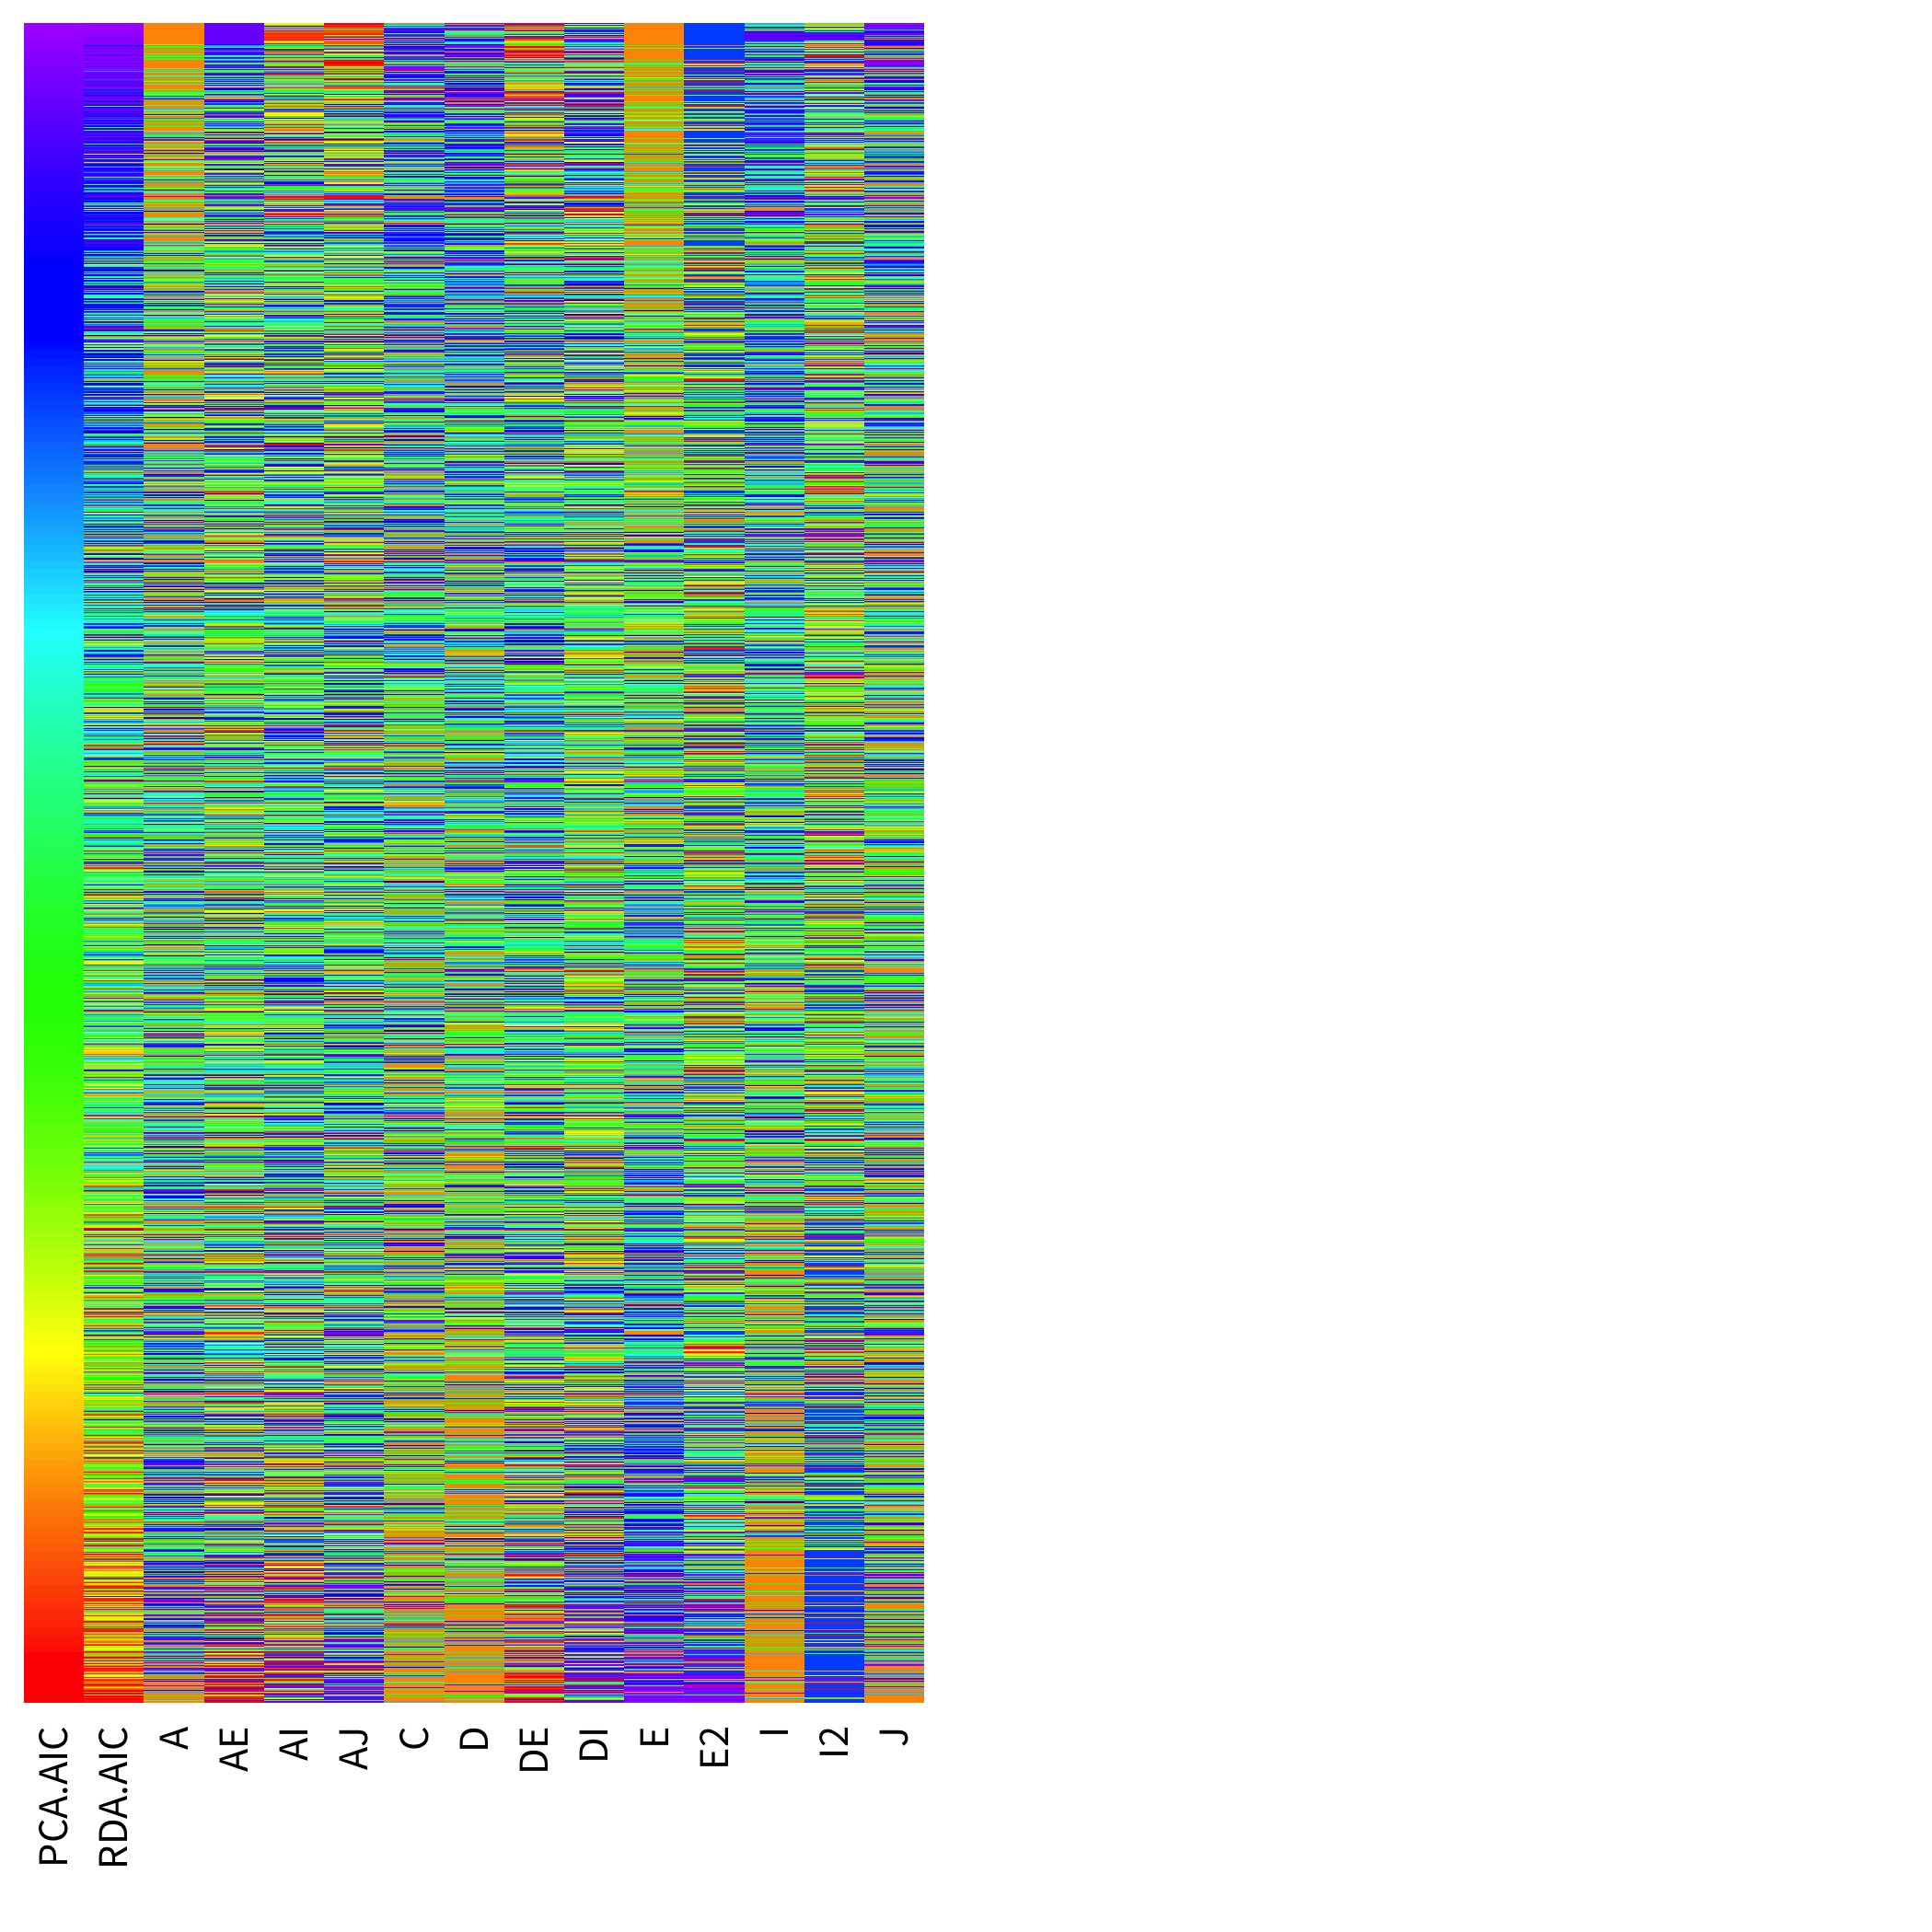
\includegraphics[angle=270, trim = 100 0 0 0, width=1\textwidth]{所有情況模擬PcaAic.png}
%\end{frame}
%
%\begin{frame}{亂數模擬500,000個樣點面積之預測:前20名(基於RDA\textsubscript{AIC})}
%% latex table generated in R 3.2.2 by xtable 1.7-4 package
%% Wed Nov  4 06:11:07 2015
%\begin{table}[ht]
%\centering
%\footnotesize
%\addfontfeatures{Numbers={Monospaced}}
%\begin{tabular}{rrrrrrrrrr}
%  \hline
% & Bio & Ga & Gb & Gc & Gd & Ge & Gf & Gi & Gj \\ 
%  \hline
%266859 & 2.33 & 0.99 & 3.59 & 1.12 & 38.35 & 11.08 & 1.71 & 1.31 & 41.85 \\ 
%  438905 & 2.06 & 3.34 & 3.98 & 2.95 & 33.26 & 13.88 & 3.69 & 1.66 & 37.24 \\ 
%  122120 & 2.06 & 1.97 & 0.65 & 3.00 & 19.71 & 40.49 & 0.45 & 1.13 & 32.60 \\ 
%  96407 & 2.03 & 1.72 & 0.36 & 4.85 & 35.39 & 14.79 & 2.35 & 7.00 & 33.54 \\ 
%  294760 & 2.03 & 5.95 & 2.52 & 2.56 & 20.88 & 19.39 & 4.11 & 1.21 & 43.38 \\ 
%  321949 & 2.01 & 4.01 & 4.79 & 5.66 & 29.28 & 19.39 & 0.97 & 0.61 & 35.28 \\ 
%  400850 & 2.01 & 5.79 & 2.48 & 0.73 & 46.02 & 8.30 & 3.39 & 0.48 & 32.80 \\ 
%  151570 & 2.01 & 4.34 & 1.03 & 7.56 & 26.83 & 18.40 & 1.38 & 2.40 & 38.06 \\ 
%  73909 & 1.99 & 6.54 & 3.15 & 2.69 & 34.31 & 16.92 & 1.76 & 1.38 & 33.26 \\ 
%  210911 & 1.96 & 1.34 & 2.99 & 3.56 & 41.23 & 13.51 & 2.08 & 7.12 & 28.17 \\ 
%  202541 & 1.96 & 1.93 & 6.23 & 2.53 & 33.54 & 18.64 & 2.53 & 3.55 & 31.07 \\ 
%  170660 & 1.94 & 2.28 & 1.09 & 13.44 & 45.47 & 5.83 & 1.14 & 0.91 & 29.83 \\ 
%  394483 & 1.93 & 5.53 & 2.67 & 1.21 & 27.58 & 19.54 & 4.62 & 3.57 & 35.29 \\ 
%  408331 & 1.92 & 0.93 & 11.63 & 3.42 & 29.37 & 12.97 & 1.12 & 3.02 & 37.53 \\ 
%  247421 & 1.92 & 5.01 & 5.16 & 0.52 & 31.26 & 29.49 & 1.67 & 0.93 & 25.96 \\ 
%  359351 & 1.91 & 1.18 & 3.63 & 4.30 & 29.31 & 28.72 & 3.37 & 2.12 & 27.37 \\ 
%  31489 & 1.91 & 3.04 & 2.43 & 7.86 & 31.75 & 16.94 & 1.98 & 3.67 & 32.34 \\ 
%  247027 & 1.91 & 2.30 & 13.60 & 1.16 & 19.74 & 26.53 & 0.18 & 0.41 & 36.08 \\ 
%  222295 & 1.91 & 2.04 & 13.01 & 3.86 & 16.03 & 15.09 & 1.19 & 2.24 & 46.53 \\ 
%  149607 & 1.89 & 1.35 & 5.40 & 5.16 & 33.08 & 6.15 & 8.49 & 1.33 & 39.03 \\    \hline
%\end{tabular}
%\end{table}
%\end{frame}
%
%
%
%\begin{frame}{亂數模擬500,000個樣點面積之預測:後20名(基於RDA\textsubscript{AIC})}
%% latex table generated in R 3.2.2 by xtable 1.7-4 package
%% Wed Nov  4 06:11:07 2015
%\begin{table}[ht]
%\centering
%\footnotesize
%\addfontfeatures{Numbers={Monospaced}}
%\begin{tabular}{rrrrrrrrrr}
%  \hline
% & Bio & Ga & Gb & Gc & Gd & Ge & Gf & Gi & Gj \\ 
%  \hline
%256233 & -1.59 & 0.03 & 40.69 & 25.75 & 0.28 & 24.66 & 3.51 & 5.05 & 0.04 \\ 
%  368541 & -1.51 & 0.06 & 25.92 & 13.45 & 0.70 & 28.83 & 21.38 & 9.62 & 0.04 \\ 
%  351608 & -1.47 & 0.71 & 34.06 & 14.35 & 0.43 & 27.98 & 10.53 & 11.19 & 0.74 \\ 
%  264358 & -1.46 & 0.52 & 0.88 & 13.53 & 0.52 & 35.22 & 0.15 & 46.01 & 3.17 \\ 
%  449632 & -1.45 & 0.32 & 24.14 & 17.91 & 0.30 & 26.59 & 30.05 & 0.23 & 0.46 \\ 
%  238150 & -1.44 & 0.03 & 29.28 & 0.32 & 0.73 & 29.08 & 27.36 & 12.03 & 1.17 \\ 
%  169328 & -1.44 & 1.22 & 2.85 & 13.60 & 1.95 & 40.18 & 2.12 & 36.68 & 1.41 \\ 
%  267986 & -1.43 & 0.61 & 27.77 & 14.78 & 0.76 & 24.79 & 19.37 & 11.67 & 0.24 \\ 
%  61554 & -1.43 & 3.03 & 27.74 & 6.56 & 0.23 & 31.27 & 26.09 & 4.13 & 0.95 \\ 
%  455348 & -1.43 & 1.77 & 3.96 & 19.38 & 1.38 & 42.46 & 6.03 & 24.32 & 0.69 \\ 
%  171870 & -1.41 & 0.80 & 23.76 & 7.21 & 1.80 & 35.39 & 10.98 & 19.26 & 0.81 \\ 
%  375725 & -1.41 & 2.16 & 26.01 & 1.79 & 0.77 & 28.64 & 22.29 & 18.04 & 0.30 \\ 
%  205794 & -1.41 & 0.29 & 29.17 & 17.92 & 0.01 & 32.95 & 6.22 & 10.86 & 2.57 \\ 
%  199168 & -1.40 & 1.03 & 15.75 & 14.71 & 0.68 & 29.31 & 9.41 & 28.31 & 0.79 \\ 
%  153275 & -1.40 & 3.78 & 38.21 & 5.25 & 0.92 & 36.82 & 6.42 & 7.97 & 0.61 \\ 
%  306424 & -1.39 & 3.74 & 29.93 & 17.04 & 0.19 & 32.11 & 4.04 & 11.85 & 1.09 \\ 
%  6730 & -1.39 & 2.51 & 11.79 & 10.90 & 1.43 & 32.73 & 10.11 & 30.27 & 0.27 \\ 
%  295092 & -1.38 & 0.22 & 30.46 & 7.14 & 0.88 & 28.38 & 11.21 & 20.37 & 1.33 \\ 
%  460996 & -1.38 & 3.71 & 37.35 & 7.77 & 2.23 & 33.68 & 13.55 & 1.20 & 0.51 \\ 
%  269597 & -1.38 & 0.17 & 15.23 & 19.83 & 0.42 & 27.54 & 12.77 & 23.19 & 0.85 \\ 
%   \hline
%\end{tabular}
%\end{table}
%\end{frame}
%
%
%\begin{frame}{亂數模擬500,000個樣點面積之預測:前20名(基於RDA.BIC)}
%% latex table generated in R 3.2.2 by xtable 1.7-4 package
%% Wed Nov  4 06:11:07 2015
%\begin{table}[ht]
%\centering
%\footnotesize
%\addfontfeatures{Numbers={Monospaced}}
%\begin{tabular}{rrrrrrrrrr}
%  \hline
% & Bio & Ga & Gb & Gc & Gd & Ge & Gf & Gi & Gj \\ 
%  \hline
%266859 & 2.38 & 0.99 & 3.59 & 1.12 & 38.35 & 11.08 & 1.71 & 1.31 & 41.85 \\ 
%  438905 & 2.09 & 3.34 & 3.98 & 2.95 & 33.26 & 13.88 & 3.69 & 1.66 & 37.24 \\ 
%  294760 & 2.09 & 5.95 & 2.52 & 2.56 & 20.88 & 19.39 & 4.11 & 1.21 & 43.38 \\ 
%  122120 & 2.09 & 1.97 & 0.65 & 3.00 & 19.71 & 40.49 & 0.45 & 1.13 & 32.60 \\ 
%  151570 & 2.06 & 4.34 & 1.03 & 7.56 & 26.83 & 18.40 & 1.38 & 2.40 & 38.06 \\ 
%  96407 & 2.06 & 1.72 & 0.36 & 4.85 & 35.39 & 14.79 & 2.35 & 7.00 & 33.54 \\ 
%  400850 & 2.05 & 5.79 & 2.48 & 0.73 & 46.02 & 8.30 & 3.39 & 0.48 & 32.80 \\ 
%  321949 & 2.03 & 4.01 & 4.79 & 5.66 & 29.28 & 19.39 & 0.97 & 0.61 & 35.28 \\ 
%  73909 & 2.02 & 6.54 & 3.15 & 2.69 & 34.31 & 16.92 & 1.76 & 1.38 & 33.26 \\ 
%  170660 & 1.97 & 2.28 & 1.09 & 13.44 & 45.47 & 5.83 & 1.14 & 0.91 & 29.83 \\ 
%  394483 & 1.96 & 5.53 & 2.67 & 1.21 & 27.58 & 19.54 & 4.62 & 3.57 & 35.29 \\ 
%  202541 & 1.96 & 1.93 & 6.23 & 2.53 & 33.54 & 18.64 & 2.53 & 3.55 & 31.07 \\ 
%  210911 & 1.95 & 1.34 & 2.99 & 3.56 & 41.23 & 13.51 & 2.08 & 7.12 & 28.17 \\ 
%  463200 & 1.94 & 0.28 & 0.88 & 8.88 & 17.44 & 19.29 & 3.89 & 5.64 & 43.70 \\ 
%  31489 & 1.93 & 3.04 & 2.43 & 7.86 & 31.75 & 16.94 & 1.98 & 3.67 & 32.34 \\ 
%  149607 & 1.92 & 1.35 & 5.40 & 5.16 & 33.08 & 6.15 & 8.49 & 1.33 & 39.03 \\ 
%  247421 & 1.90 & 5.01 & 5.16 & 0.52 & 31.26 & 29.49 & 1.67 & 0.93 & 25.96 \\ 
%  359351 & 1.90 & 1.18 & 3.63 & 4.30 & 29.31 & 28.72 & 3.37 & 2.12 & 27.37 \\ 
%  347887 & 1.90 & 2.65 & 2.34 & 0.47 & 29.95 & 22.56 & 12.29 & 0.37 & 29.38 \\ 
%  408331 & 1.88 & 0.93 & 11.63 & 3.42 & 29.37 & 12.97 & 1.12 & 3.02 & 37.53 \\ 
%   \hline
%\end{tabular}
%\end{table}
%\end{frame}
%
%
%
%
%\begin{frame}{亂數模擬500,000個樣點面積之預測:後20名(基於RDA.BIC)}
%% latex table generated in R 3.2.2 by xtable 1.7-4 package
%% Wed Nov  4 06:11:07 2015
%\begin{table}[ht]
%\centering
%\footnotesize
%\addfontfeatures{Numbers={Monospaced}}
%\begin{tabular}{rrrrrrrrrr}
%  \hline
% & Bio & Ga & Gb & Gc & Gd & Ge & Gf & Gi & Gj \\ 
%  \hline
%264358 & -1.51 & 0.52 & 0.88 & 13.53 & 0.52 & 35.22 & 0.15 & 46.01 & 3.17 \\ 
%  169328 & -1.47 & 1.22 & 2.85 & 13.60 & 1.95 & 40.18 & 2.12 & 36.68 & 1.41 \\ 
%  455348 & -1.47 & 1.77 & 3.96 & 19.38 & 1.38 & 42.46 & 6.03 & 24.32 & 0.69 \\ 
%  73840 & -1.36 & 1.87 & 5.45 & 14.83 & 1.59 & 38.83 & 16.47 & 20.20 & 0.74 \\ 
%  165776 & -1.30 & 4.93 & 2.17 & 16.61 & 2.75 & 32.99 & 2.94 & 37.33 & 0.29 \\ 
%  203535 & -1.29 & 0.34 & 10.19 & 15.27 & 0.33 & 36.38 & 22.33 & 13.03 & 2.11 \\ 
%  6730 & -1.29 & 2.51 & 11.79 & 10.90 & 1.43 & 32.73 & 10.11 & 30.27 & 0.27 \\ 
%  238747 & -1.28 & 4.69 & 3.73 & 4.54 & 1.75 & 37.04 & 17.20 & 29.60 & 1.46 \\ 
%  78955 & -1.28 & 4.75 & 4.86 & 2.65 & 0.22 & 33.82 & 32.14 & 20.41 & 1.14 \\ 
%  428878 & -1.27 & 0.95 & 6.76 & 25.31 & 0.91 & 27.33 & 12.18 & 26.01 & 0.54 \\ 
%  392835 & -1.27 & 4.35 & 1.00 & 28.06 & 1.56 & 28.96 & 5.50 & 30.38 & 0.19 \\ 
%  165310 & -1.26 & 5.10 & 5.70 & 12.20 & 0.50 & 31.11 & 26.64 & 18.73 & 0.03 \\ 
%  50197 & -1.25 & 5.14 & 0.03 & 15.31 & 0.58 & 29.82 & 21.70 & 26.35 & 1.07 \\ 
%  269597 & -1.25 & 0.17 & 15.23 & 19.83 & 0.42 & 27.54 & 12.77 & 23.19 & 0.85 \\ 
%  98753 & -1.25 & 3.98 & 11.48 & 9.10 & 0.65 & 29.33 & 11.89 & 33.18 & 0.39 \\ 
%  199168 & -1.25 & 1.03 & 15.75 & 14.71 & 0.68 & 29.31 & 9.41 & 28.31 & 0.79 \\ 
%  471995 & -1.25 & 2.76 & 10.30 & 8.35 & 0.44 & 28.34 & 21.69 & 27.29 & 0.83 \\ 
%  450811 & -1.24 & 0.60 & 6.22 & 6.70 & 3.01 & 31.22 & 24.03 & 27.76 & 0.46 \\ 
%  45655 & -1.24 & 1.89 & 1.55 & 7.33 & 3.68 & 34.67 & 21.82 & 28.21 & 0.84 \\ 
%  428054 & -1.24 & 3.06 & 3.97 & 39.10 & 0.65 & 37.64 & 4.65 & 9.22 & 1.71 \\ 
%   \hline
%\end{tabular}
%\end{table}
%\end{frame}
%

\begin{frame}{筆記、其它解決方案及未來工作}
\begin{itemize}
	\item 不考慮未定義面積(目前辦法)及考慮未定義面積的預測能力差不多
	\item 嘗試過合併(加總)太多零的面積類別,但沒有效果
	\item 交叉驗證的 NRMSE 之間不能直接比較
	\item 需要完全檢查生態資料
	\item 需要完全檢查怪異的面積資料
	\item 自動化變數選擇應該必須避免,但已有部份改善
	\item 模型預測效果不佳,可以再找新的建模方法(如二階式迴歸)、數據(如大樣區的總面積)、以別的「角度」採用面積資料(如採用$B-A$、$frac{B}{A}$之類的面積變數)
\end{itemize}
\end{frame}



\end{document}






%\DeclareOptionBeamer{aspectratio}[43]{%
%  \ifnum#1=1610% 16:10
%    \beamer@paperwidth 16.00cm%
%    \beamer@paperheight 10.00cm%
%  \else\ifnum#1=169% 16:9
%    \beamer@paperwidth 16.00cm%
%    \beamer@paperheight 9.00cm%
%  \else\ifnum#1=149% 14:9
%    \beamer@paperwidth 14.00cm%
%    \beamer@paperheight 9.00cm%
%  \else\ifnum#1=54% 5:4
%    \beamer@paperwidth 12.50cm%
%    \beamer@paperheight 10.00cm%
%  \else\ifnum#1=43% 4:3
%    \beamer@paperwidth 12.80cm%
%    \beamer@paperheight 9.60cm%
%  \else\ifnum#1=32% 3:2
%    \beamer@paperwidth 13.50cm%
%    \beamer@paperheight 9.00cm%
%  \fi\fi\fi\fi\fi\fi%
%}
